\subsection{Fitting and Alignment with GBL.}
There are many detail associated with the track fitting and alignment which has much documentation written about it already. The algorithms used for track fitting and alignment in this case can be found here:
\newline	
\url{https://www.wiki.terascale.de/images/6/6b/Gbl_man.pdf}
\newline
\url{http://www.desy.de/~blobel/Mptwo.pdf}
\newline
How each algorithm is used can vary drastically, since all they are are algorithms for a certain purpose. GBL is simply a minimisation procedure designed exclusively for track fitting. Millepede is a minimisation procedure for a residual (Any Gaussian process) which can be linked to global parameters which are defined via partial derivatives. With this said, it is good to keep in mind the extent of both procedures. GBL will be useful for any tracking framework. Millepede will be useful for systems with a many Gaussian residuals linked together with the same global parameters, an example being the residuals on a plane and the x-shift of the plane.


This manual will hopefully shed some light on what is the basic requirements for using the software and show how this is implemented specifically in EUTelescope. The construction of a track which can be used for alignment or analysis is done in five steps. The order does not pattern except the linking of trajectory points must be done before anything else. Each step will be covered in turn. 
\section{The five fold way}
\subsection{Linking trajectory points}
The initial requirement for track fitting is a coordinate system which links the local and global frames. The local frame is defined by the readout layout of the sensor, a cartesian grid over the surface of the sensor and is unique for each DUT. The global frame is a cartesian grid which extends over the full detector system. This is the same for all DUTs and alignment is needed to link both these frame for each DUT. Each plane is linked to the same global frame using the transformation:
\begin{equation}
 \overrightarrow{G} =   \hat{R}\overrightarrow{L} +  \overrightarrow{O}
\end{equation}

were the rotation matrix is defined

\begin{equation}
 \hat{R} = \hat{R_Y}\hat{R_X}\hat{R_Z}\hat{R_I}
\end{equation}

with $R_{X/Y/Z}$ as rotations in that particular axis. $R_I$ is the initial rotation matrix which can be set in gear to whatever value you see fit. Note the offsets are defined in the global frame since they are applied after all rotations. 

The order of applying transformations matters and must be considered. This is important for alignment and is discussed in section \ref{gloPar}. All large rotations round the X/Y axis must be applied as parity transform to the initial matrix. If you apply this transform to $R_Y$, $R_X$ then the alignment matrix will not correspond to the correct from frame for the rotation corrections. The small changes to the rotations from alignment is applied to $hat{R_Z}$,  $hat{R_Y}$ and $\hat{R_X}$.


The full trajectory of a track does not need to be modelled for an accurate fit. Locations of high scattering and with measurements must be added. These points must be linked together using some Jacobain. A Jacobain in this case is just a link between how changes in position/incidence on one plane affects another. The Jacobain used to link the points together is 

\[ \left( \begin{array}{cccccc}
1                            & 0       & 0        & 0 & 0  \\
\frac{bF(0)ds}{dz} & 1        & 0        & 0 & 0  \\
\frac{bF(1)ds}{dz} & 0        & 1        & 0 & 0  \\
0.5bF(0)ds^2        & dz*ds & 0        & 1 & 0      \\  
0.5bF(1)ds^2        & 0        & dz*ds & 0 &  1       \\  
  \label{eq:PC}
\end{array}
 \right)\] 

\begin{figure}[H]
\centering
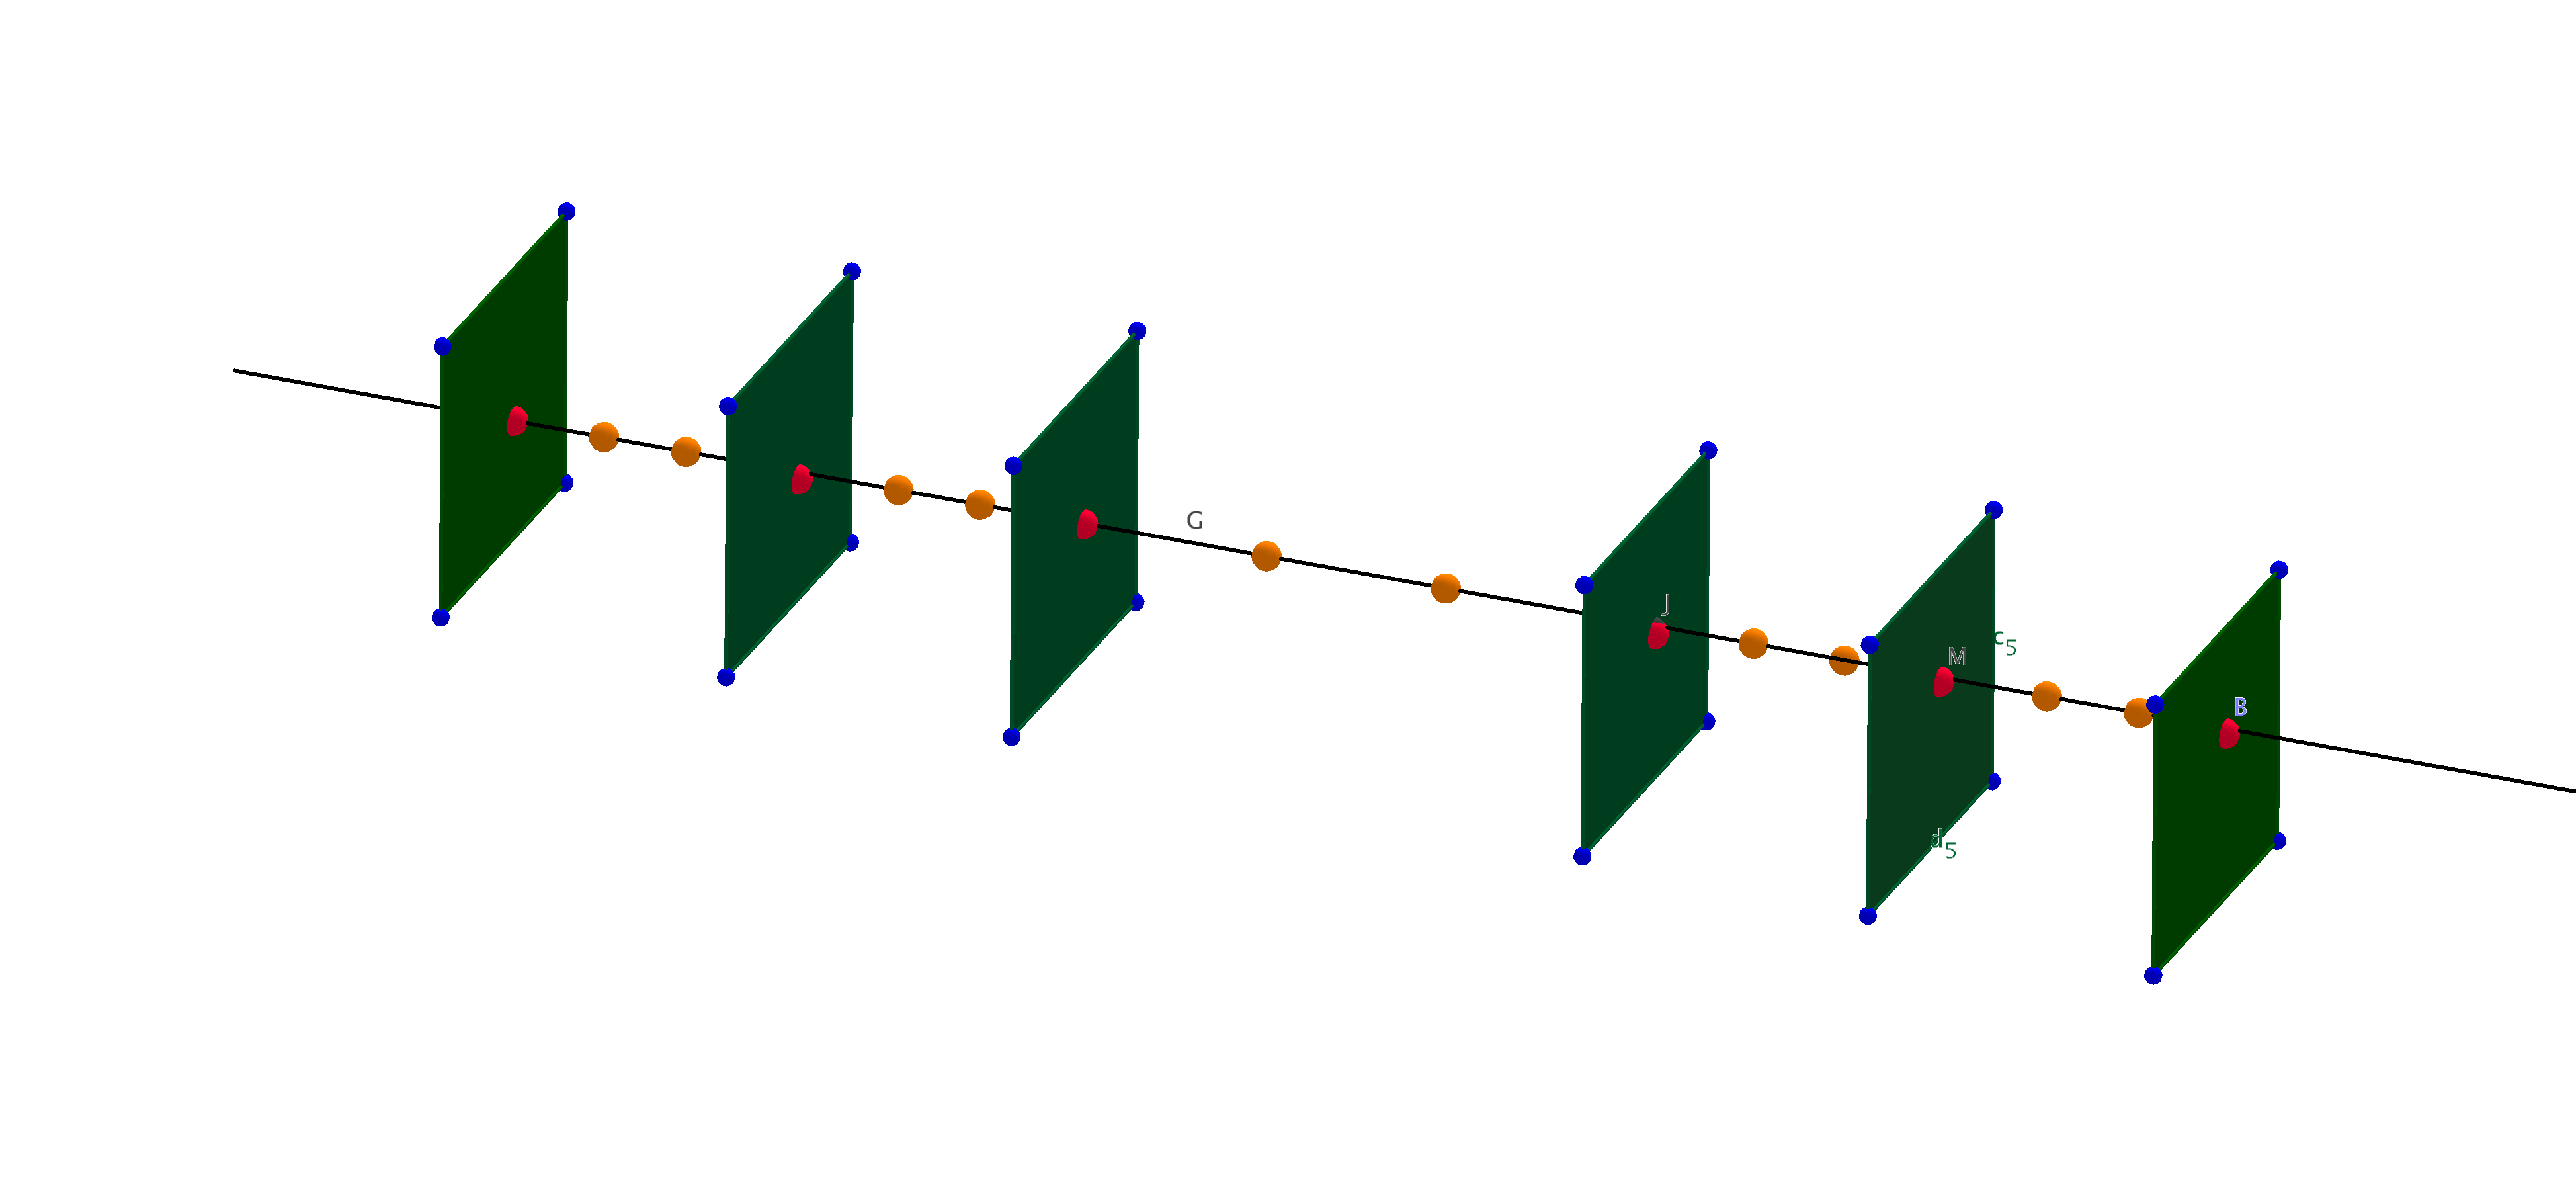
\includegraphics[width=1.0\linewidth]{figures/meas-scat-jac-link.png}
\caption{The red points have measurement and scattering information. The yellow point only scattering information. Measurements are the hit positions in the local frame. Scattering information is the kink angles measured in the local frame. Both have associated errors which must be determined.}
\label{fig:LinkJac}
\end{figure}


What points and were depend on the location of the measurements planes and the scattering from all the material. In the EUTelescope case a single point is used for each measurement and the material infront of this until the next measurement is associated with two points. Two points are need to describe a thick scatterer which is discussed in section \ref{sec:scat}.

The linking of the full trajectory is done in the global frame.

\subsection{Add measurement information to points}

With the trajectory described the measurements on the planes must be added. The measurements are the residuals (Measured-Predicted) and the associated errors. The trajectory is always in the global frame and each measurement plane will not always be in this frame. Therefore propagation between the global and local frame is needed to link this information.
The propagation matrix used is

\[ 
\left( \begin{array}{ccc}
1  & 0   & -\frac{dx}{dz}   \\
0   & 1  & -\frac{dy}{dz}  
  \label{eq:prop}
\end{array}
 \right)
  \left( \begin{array}{cc}
 \overrightarrow{Rx}  &  \overrightarrow{Ry}  
\end{array}
 \right)
 \] 
 
 with slope defined in the local frame.  $\overrightarrow{Rx}$ and  $\overrightarrow{Ry}$ are the local X/Y axis defined in the global frame. The first matrix will transform the position from global to local frame. You only need to apply the partial rotation matrix since there should be no z displacement in this frame. The second part will determine the intersection on the XY plane in the local frame from track propagated to new local position.
 
 \begin{figure}[H]
\centering
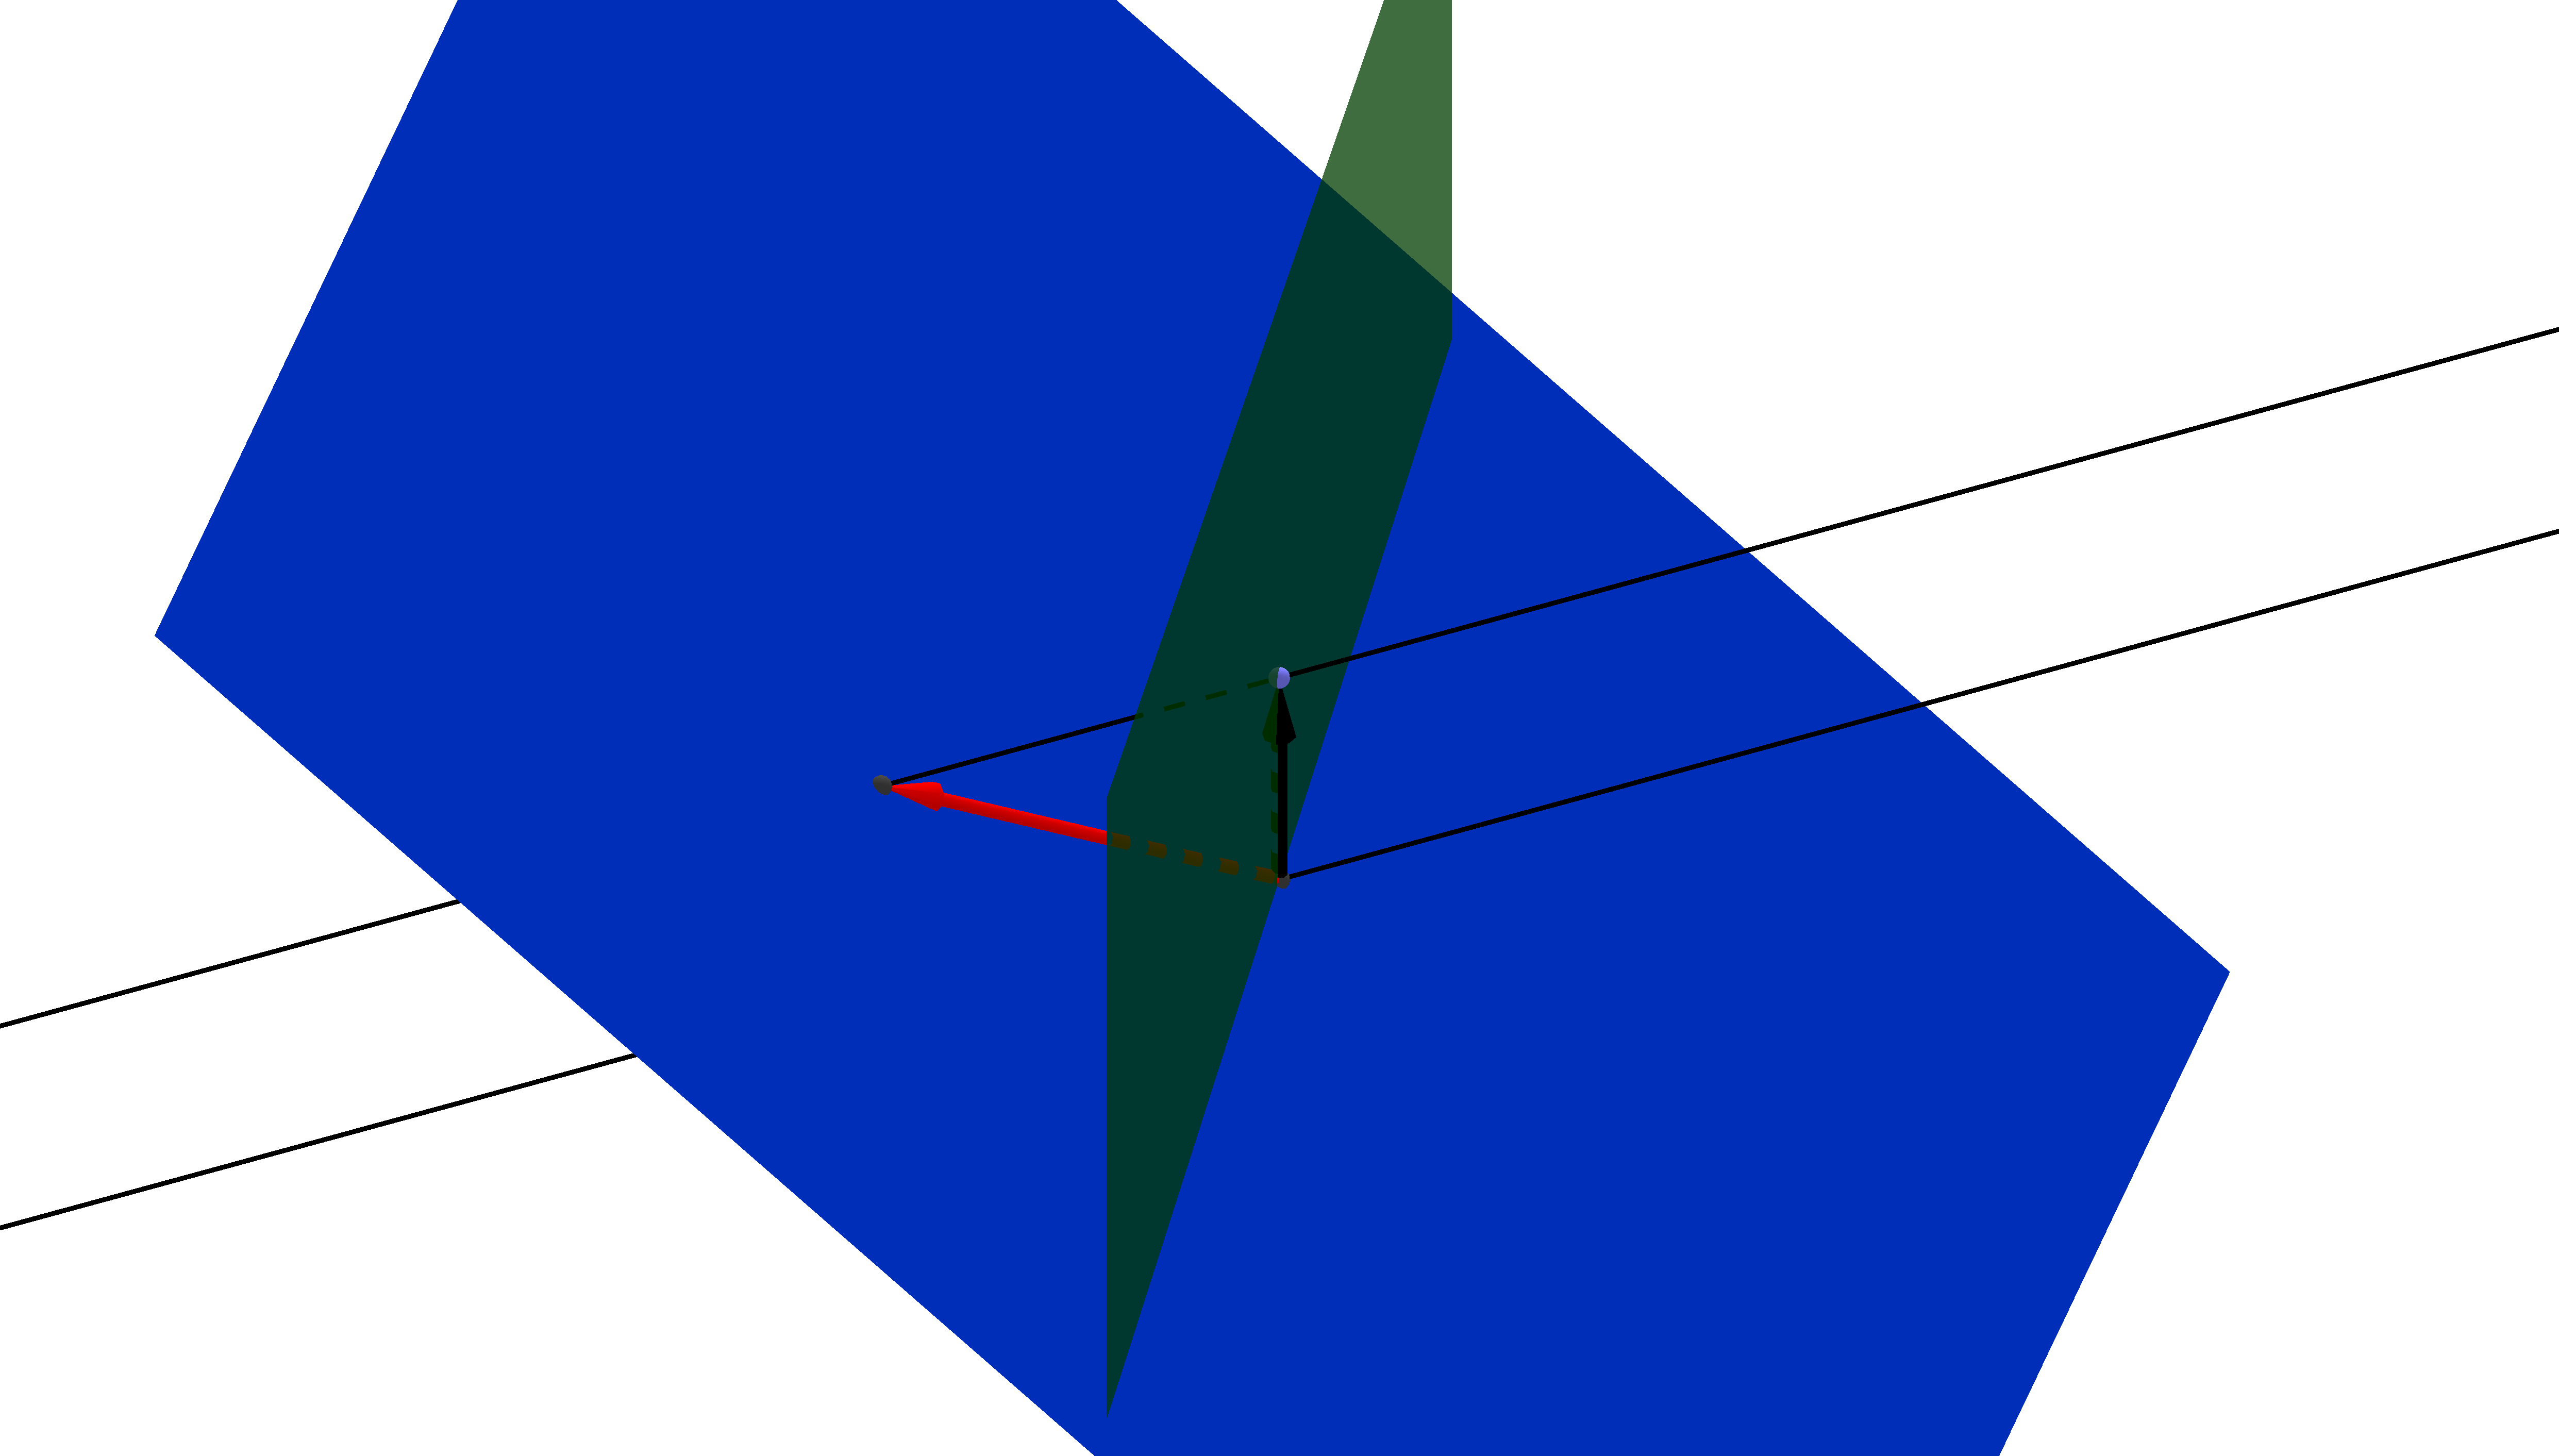
\includegraphics[width=1.0\linewidth]{figures/prop.png}
\caption{The projection matrix will relate the change in residual (black vector) in global XY plane to local XY plane (Blue plane). The propagation must take into account the change in track position intersection   }
\label{fig:Prop}
\end{figure}
 
GBL expects a link which goes from global to local and this defines the parameters used above. You can define the slopes in the local frame and axis in global frame and then invert the corresponding matrix. Either or will work.



\subsection{Add scattering information}
\label{sec:scat}
Scattering in the EUTelescope framework is always assumed to be thin (Discussed later). Furthermore the scattering error will non be diagonal in the local frame of the sensor. The propagation matrix from the frame parallel to the track and local frame is

\[ 
\frac{\theta_{0}^{2}}{1-c^2_1 c^2_2}
\left(
  \begin{array}{cc}
 1-c^{2}_{2} & c_{1}c_{2}    \\
 c_{1}c_{2} & 1-c^{2}_{1} \\   
\end{array} \right)\] 



This propagation is shown by \ref{fig:ScatFrame} with the plane perpendicular to the track containing the diagonal error matrix. However if the matrix is transformed to the plane frame (Blue plane \ref{fig:ScatFrame}) then the error matrix will be non diagonal.

\begin{figure}[H]
\centering
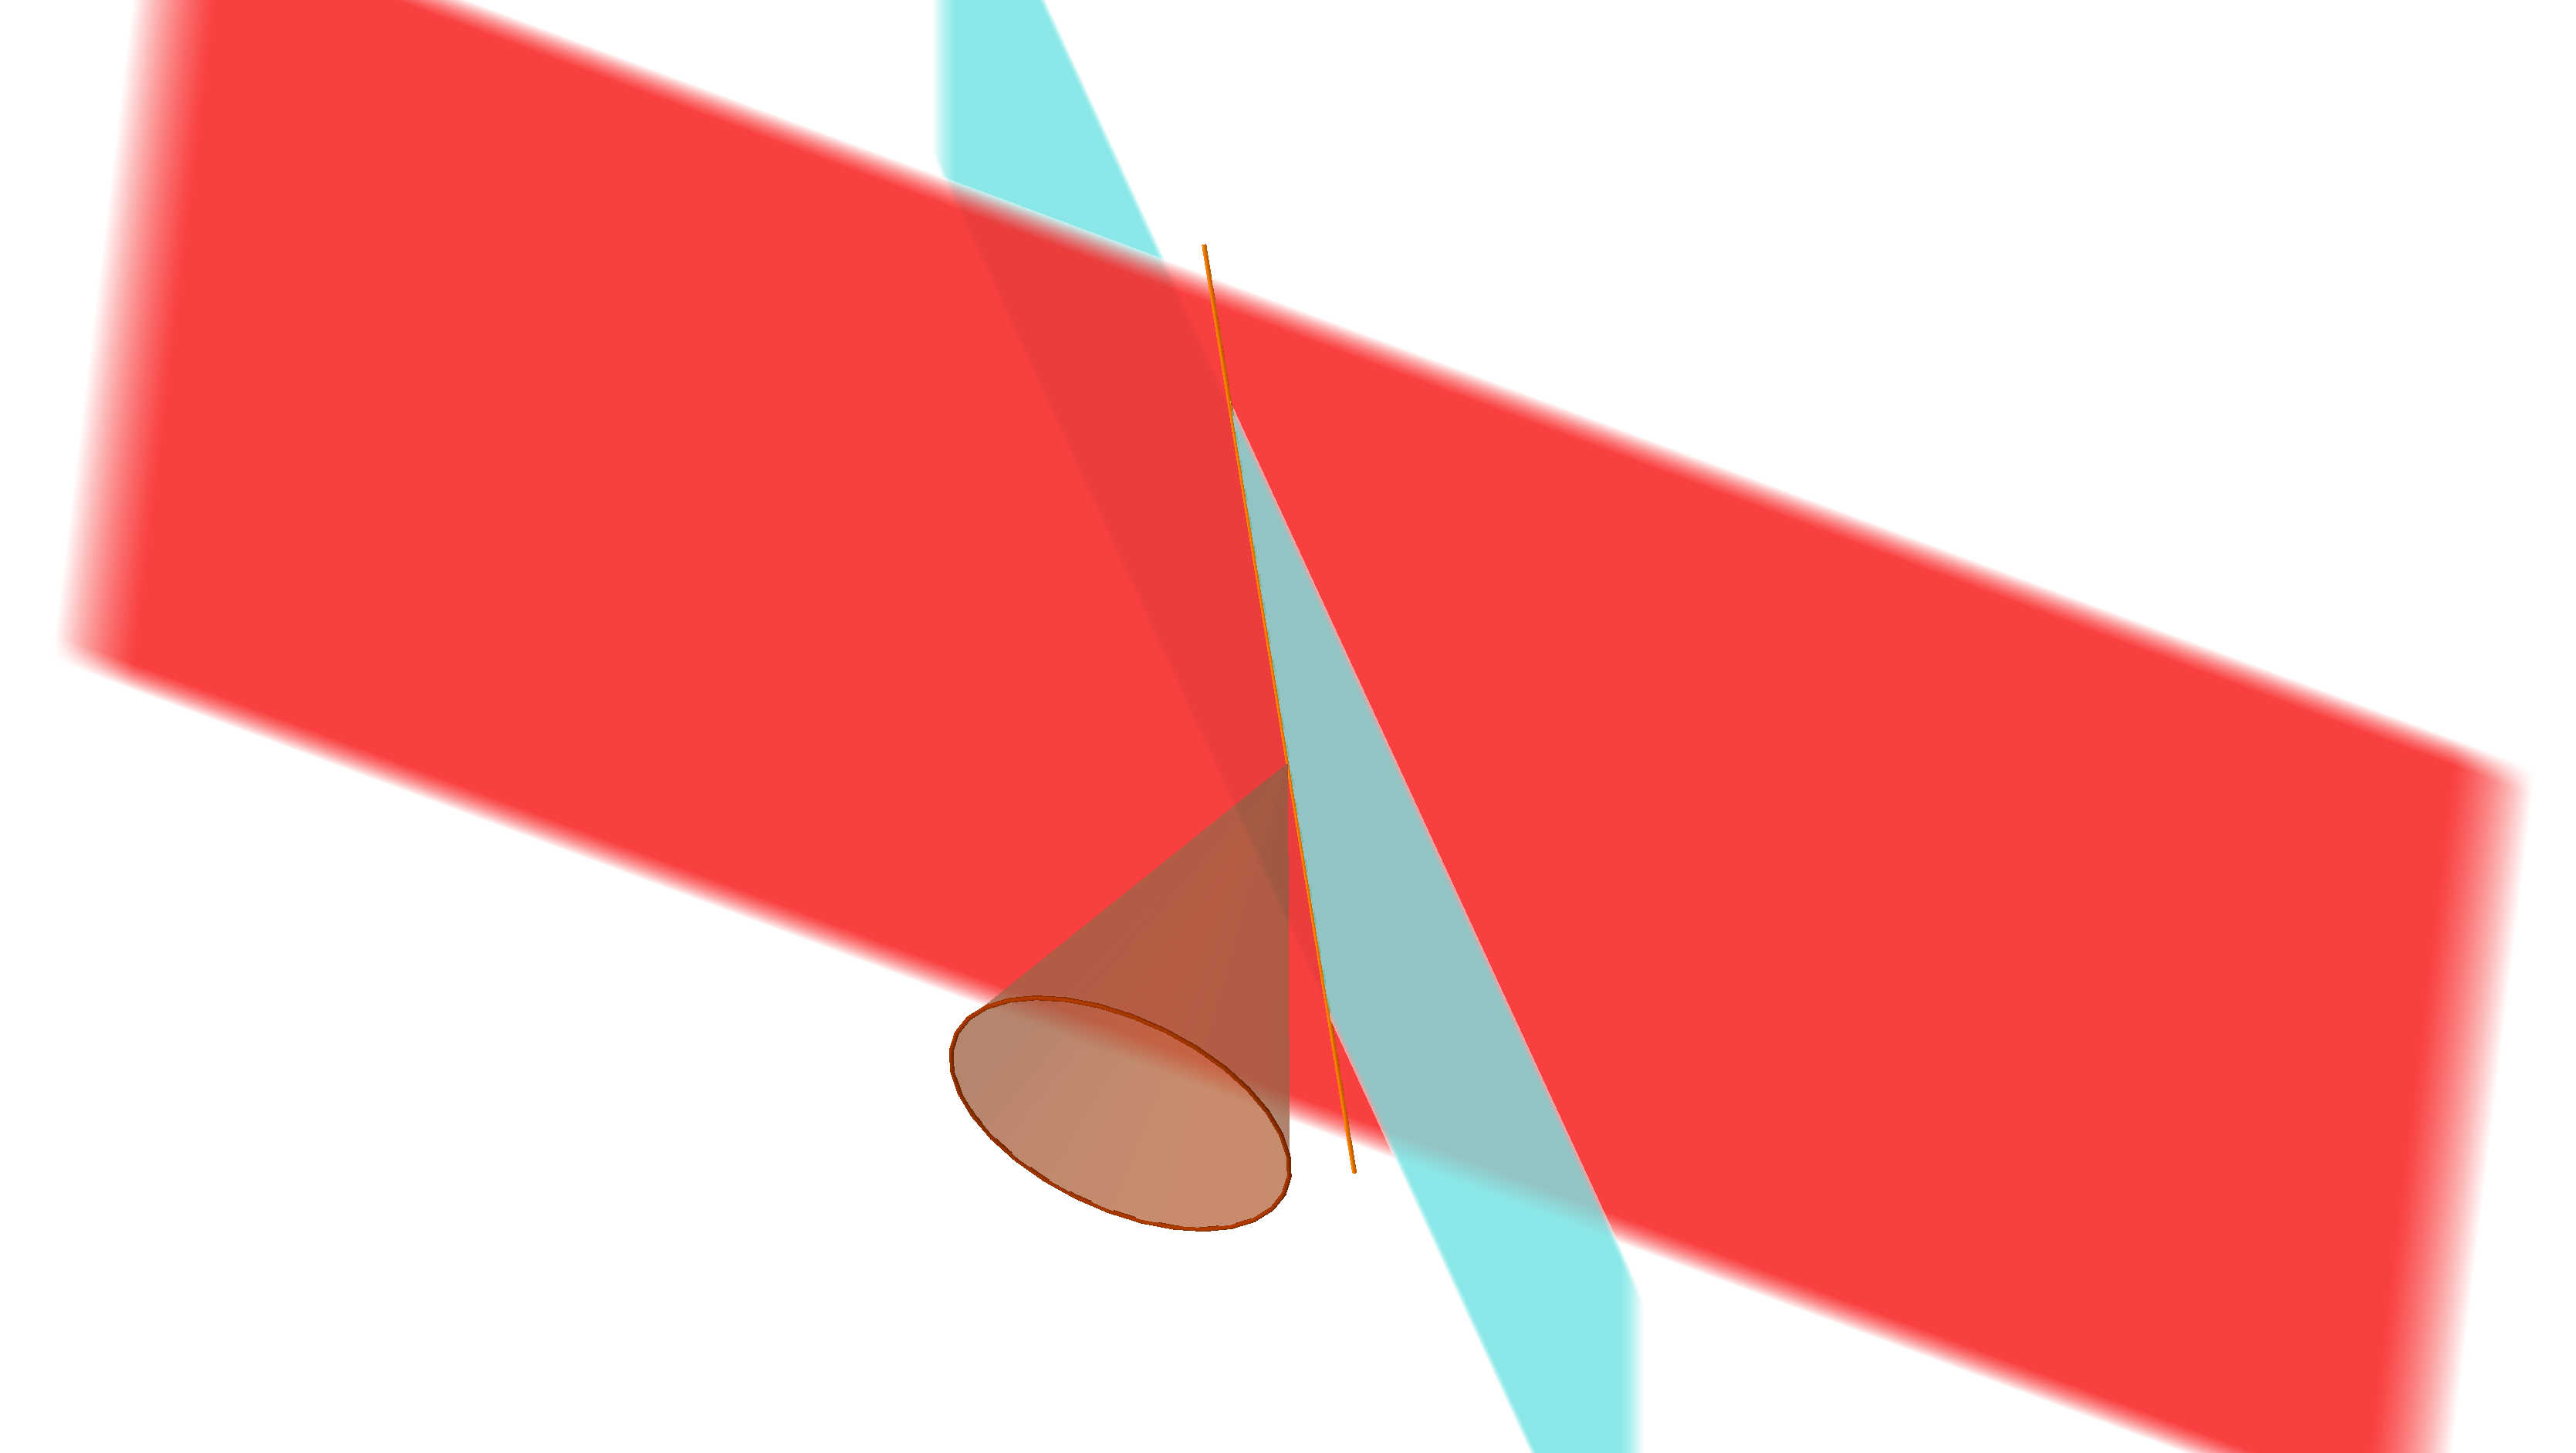
\includegraphics[width=1.0\linewidth]{figures/propGood600.png}
\caption{The scattering frame is the red plane which is perpendicular to the track. The blue plane is the sensor surface. Compare the circular cone which has a diagonal error matrix to the ellipsoid which is non diagonal. This ellipsoid is better seen if the XY plane is propagated downstream with the errors \ref{fig:ScatFrame1}.}
\label{fig:ScatFrame}
\end{figure}

The view of the errors associated from scattering on the plane is shown in figures \ref{fig:ScatFrame1} and \ref{fig:ScatFrame2}. 

\begin{figure}[H]
\centering
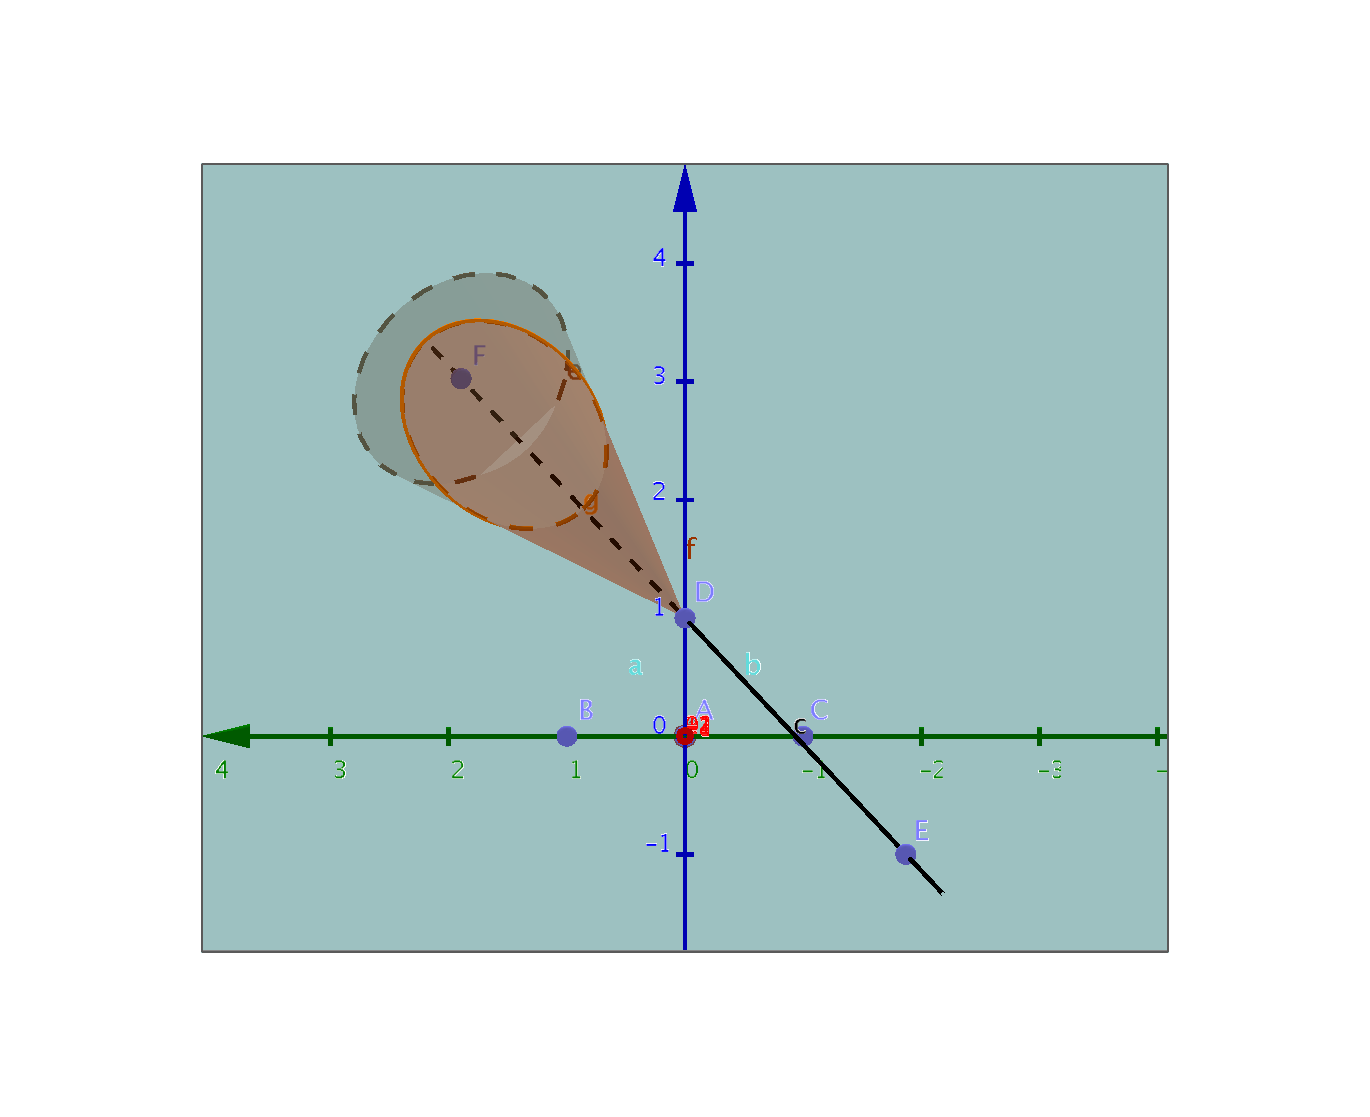
\includegraphics[width=1.0\linewidth]{figures/scatterDownZProjection.png}
\caption{The scattering cone projected on the XY plane of the sensor. The errors on the sensor must take this form to propagate correctly in the z axis}
\label{fig:ScatFrame1}
\end{figure}

\begin{figure}[H]
\centering
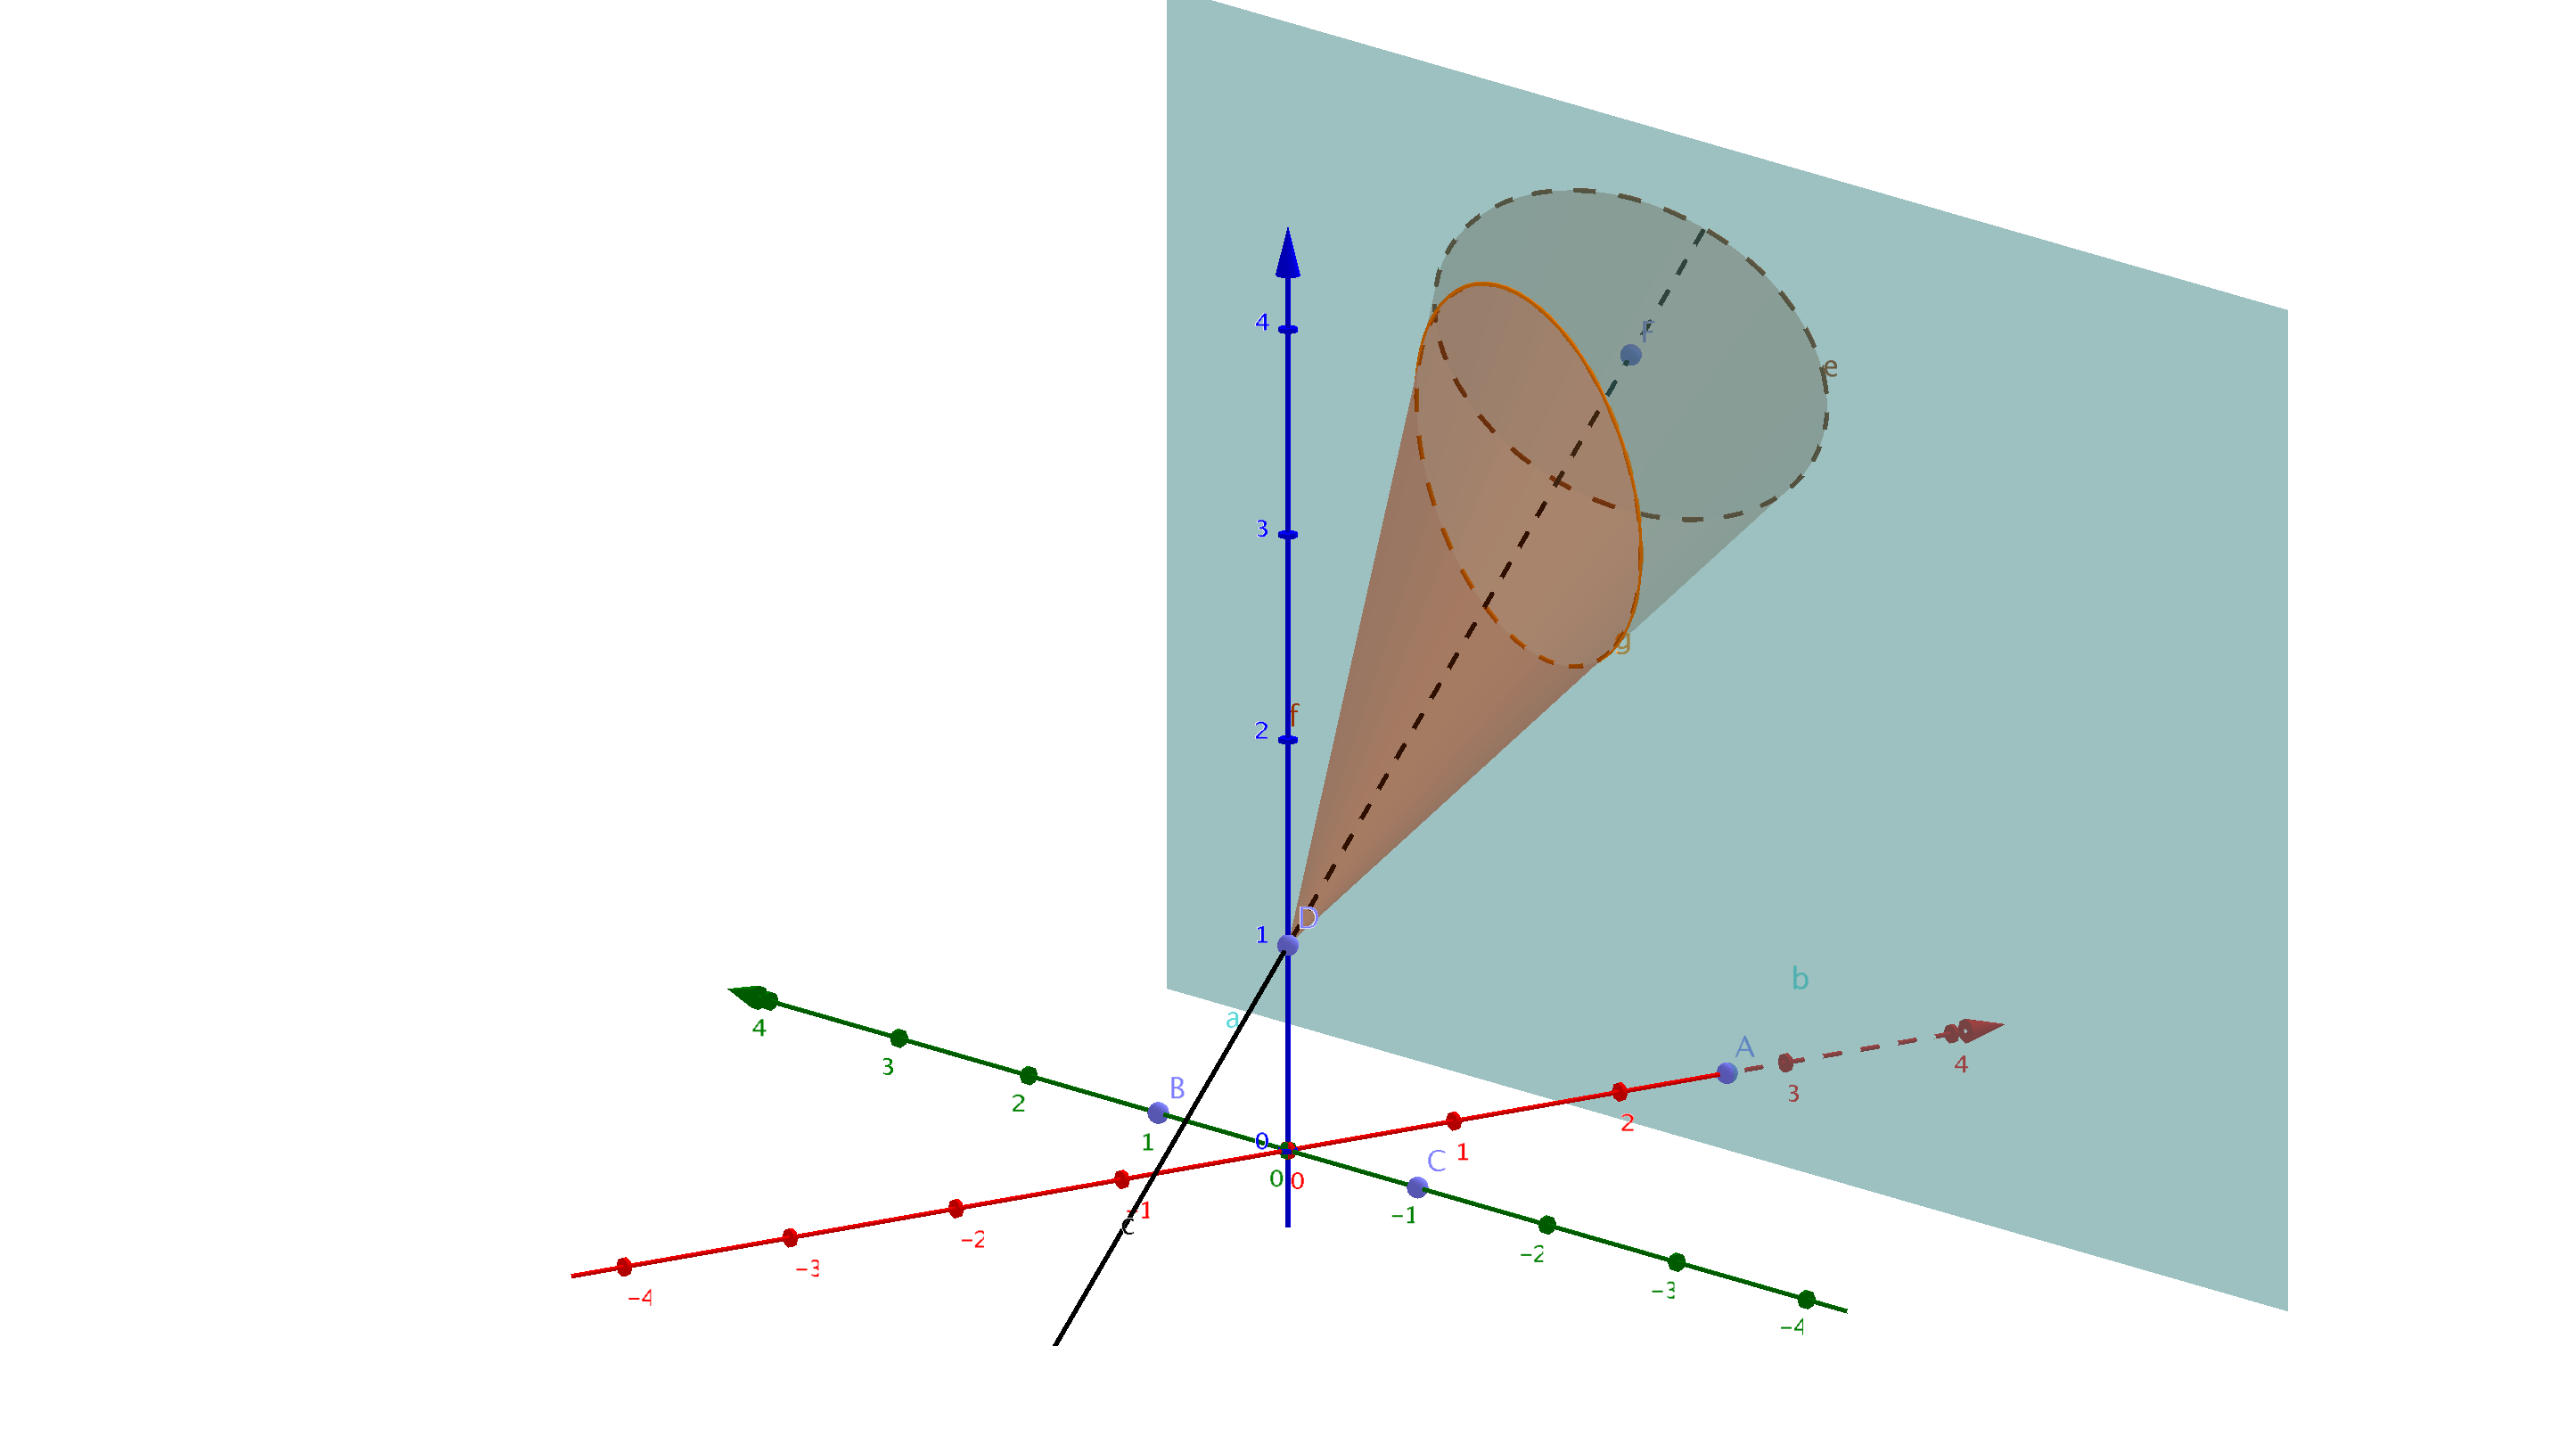
\includegraphics[width=1.0\linewidth]{figures/prop600GoodOffSensor.png}
\caption{The same as figure \ref{fig:ScatFrame1} from a different angle.}
\label{fig:ScatFrame2}
\end{figure}

The propagation of scattering errors to different frames is all well and good. However you must be able to determine the amount of scattering expected at each point.

First the total radiation length must be determined for the track's trajectory. TGeo volumes are used to describe the full detector system including the radiation length. The track is assumed to propagate through each volume at the appropriate incidence to determine the correct radiation length at each point. Two things must be determined to model scattering.

First the variance at each point must be determined. To determine this the total variance of the trajectory must be calculated. The total variance is calculated using the radiation length and beam energy. This is were the Highland formula comes in. The Highland formula relates the radiation length percentage and beam energy to a scattering RMS. One important characteristic of the HIghland formula is its non linear properties: The radiation length calculated must be for the full system and then split between each point used to model the scattering. 

Second the position of the scatterers must be determined. This depends on the radiation length and size of the volume to model. If the volume is thin then it can be assumed a thin scatterer. A thin scatter will have no displacement through the material but some angular displacement. So all the radiation length is located at that point. The red measurement dots on figure \ref{fig:LinkJac} are modelled this way. The variance at this point is the total weighted by the fraction at this point relative to the total radiation length.
A thick scatterer which will have some displacement due to scattering within the material and can be viewed as the combination of many thin scatterers. If you propagate the error associated with each thin scatterer which makes up the thick scatter then it can be shown that a thick scatterer can be modelled by two thin scatterers. The location and allowed variance of the kinks is determined using the relations

\begin{multicols}{2}
\begin{equation}
 s_1 = s_0
\end{equation}
\begin{equation}
s_2 = \overline{s} + \frac{\Delta s^{2}}{\overline s - s_1} 
\end{equation}
\begin{equation}
\theta_{1}^{2} = \theta^{2}\frac{\Delta s^{2}}{(\Delta s^2 + (\overline s - s_1)^{2}} 
\end{equation}
\begin{equation}
\theta_{2} = \theta^{2}\frac{(\overline s - s_1)^{2}}{\Delta s^2 + (\overline s - s_1)^2} 
\end{equation}
\end{multicols}

were $\theta$ is the total variance, $s_0$ as the initial position of the scattering volume and 

\begin{multicols}{3}
\begin{equation}
\theta^{2} = \int_{a}^{b} \theta_{i}^{2}
\end{equation}
\begin{equation}
\overline{s}=\frac{\int_{a}^{b} s_i \theta_{i}^{2}}{\theta^2}
\end{equation}
\begin{equation}
\Delta s^{2} = \frac{\int_{a}^{b} ( s_i  - \overline{s})^2 \theta^{2}_{i}}{\theta^2}
\end{equation}
\end{multicols}

were T=b-a which is the start and end position of the scatter volume. 
Integration can be used to work out the parameter values for any inhomogeneous volumes. Most situation will have blocks of homogeneous material one after the other. In this case the above equation can be treated as: 

\begin{equation}
 \overline{s} = 0.5 \sum_i \frac{T_i}{X0_i} 
\end{equation}

\begin{equation}
 \Delta s^{2} = \sum_i \frac{\frac{1}{3} T^3 - T^{2}\overline{s} + T\overline{s}^{2}}{X0_i} 
\end{equation}

\begin{equation}
 norm =   \frac{T_i}{X0_i} 
\end{equation}

were T is the thickness and the summation is over all homogenous volumes.  



\subsection{Add global parameters}
\label{gloPar}
The addition of global parameters is used for alignment parameters. However this can be used for any situation to determine parameters which are linked to all the track parameters. Note this in contrast to local parameters which vary from track to track.  Alignment is simply the determination of the correct transformation from local to global frames for each sensor. 

\begin{figure}[H]
\centering
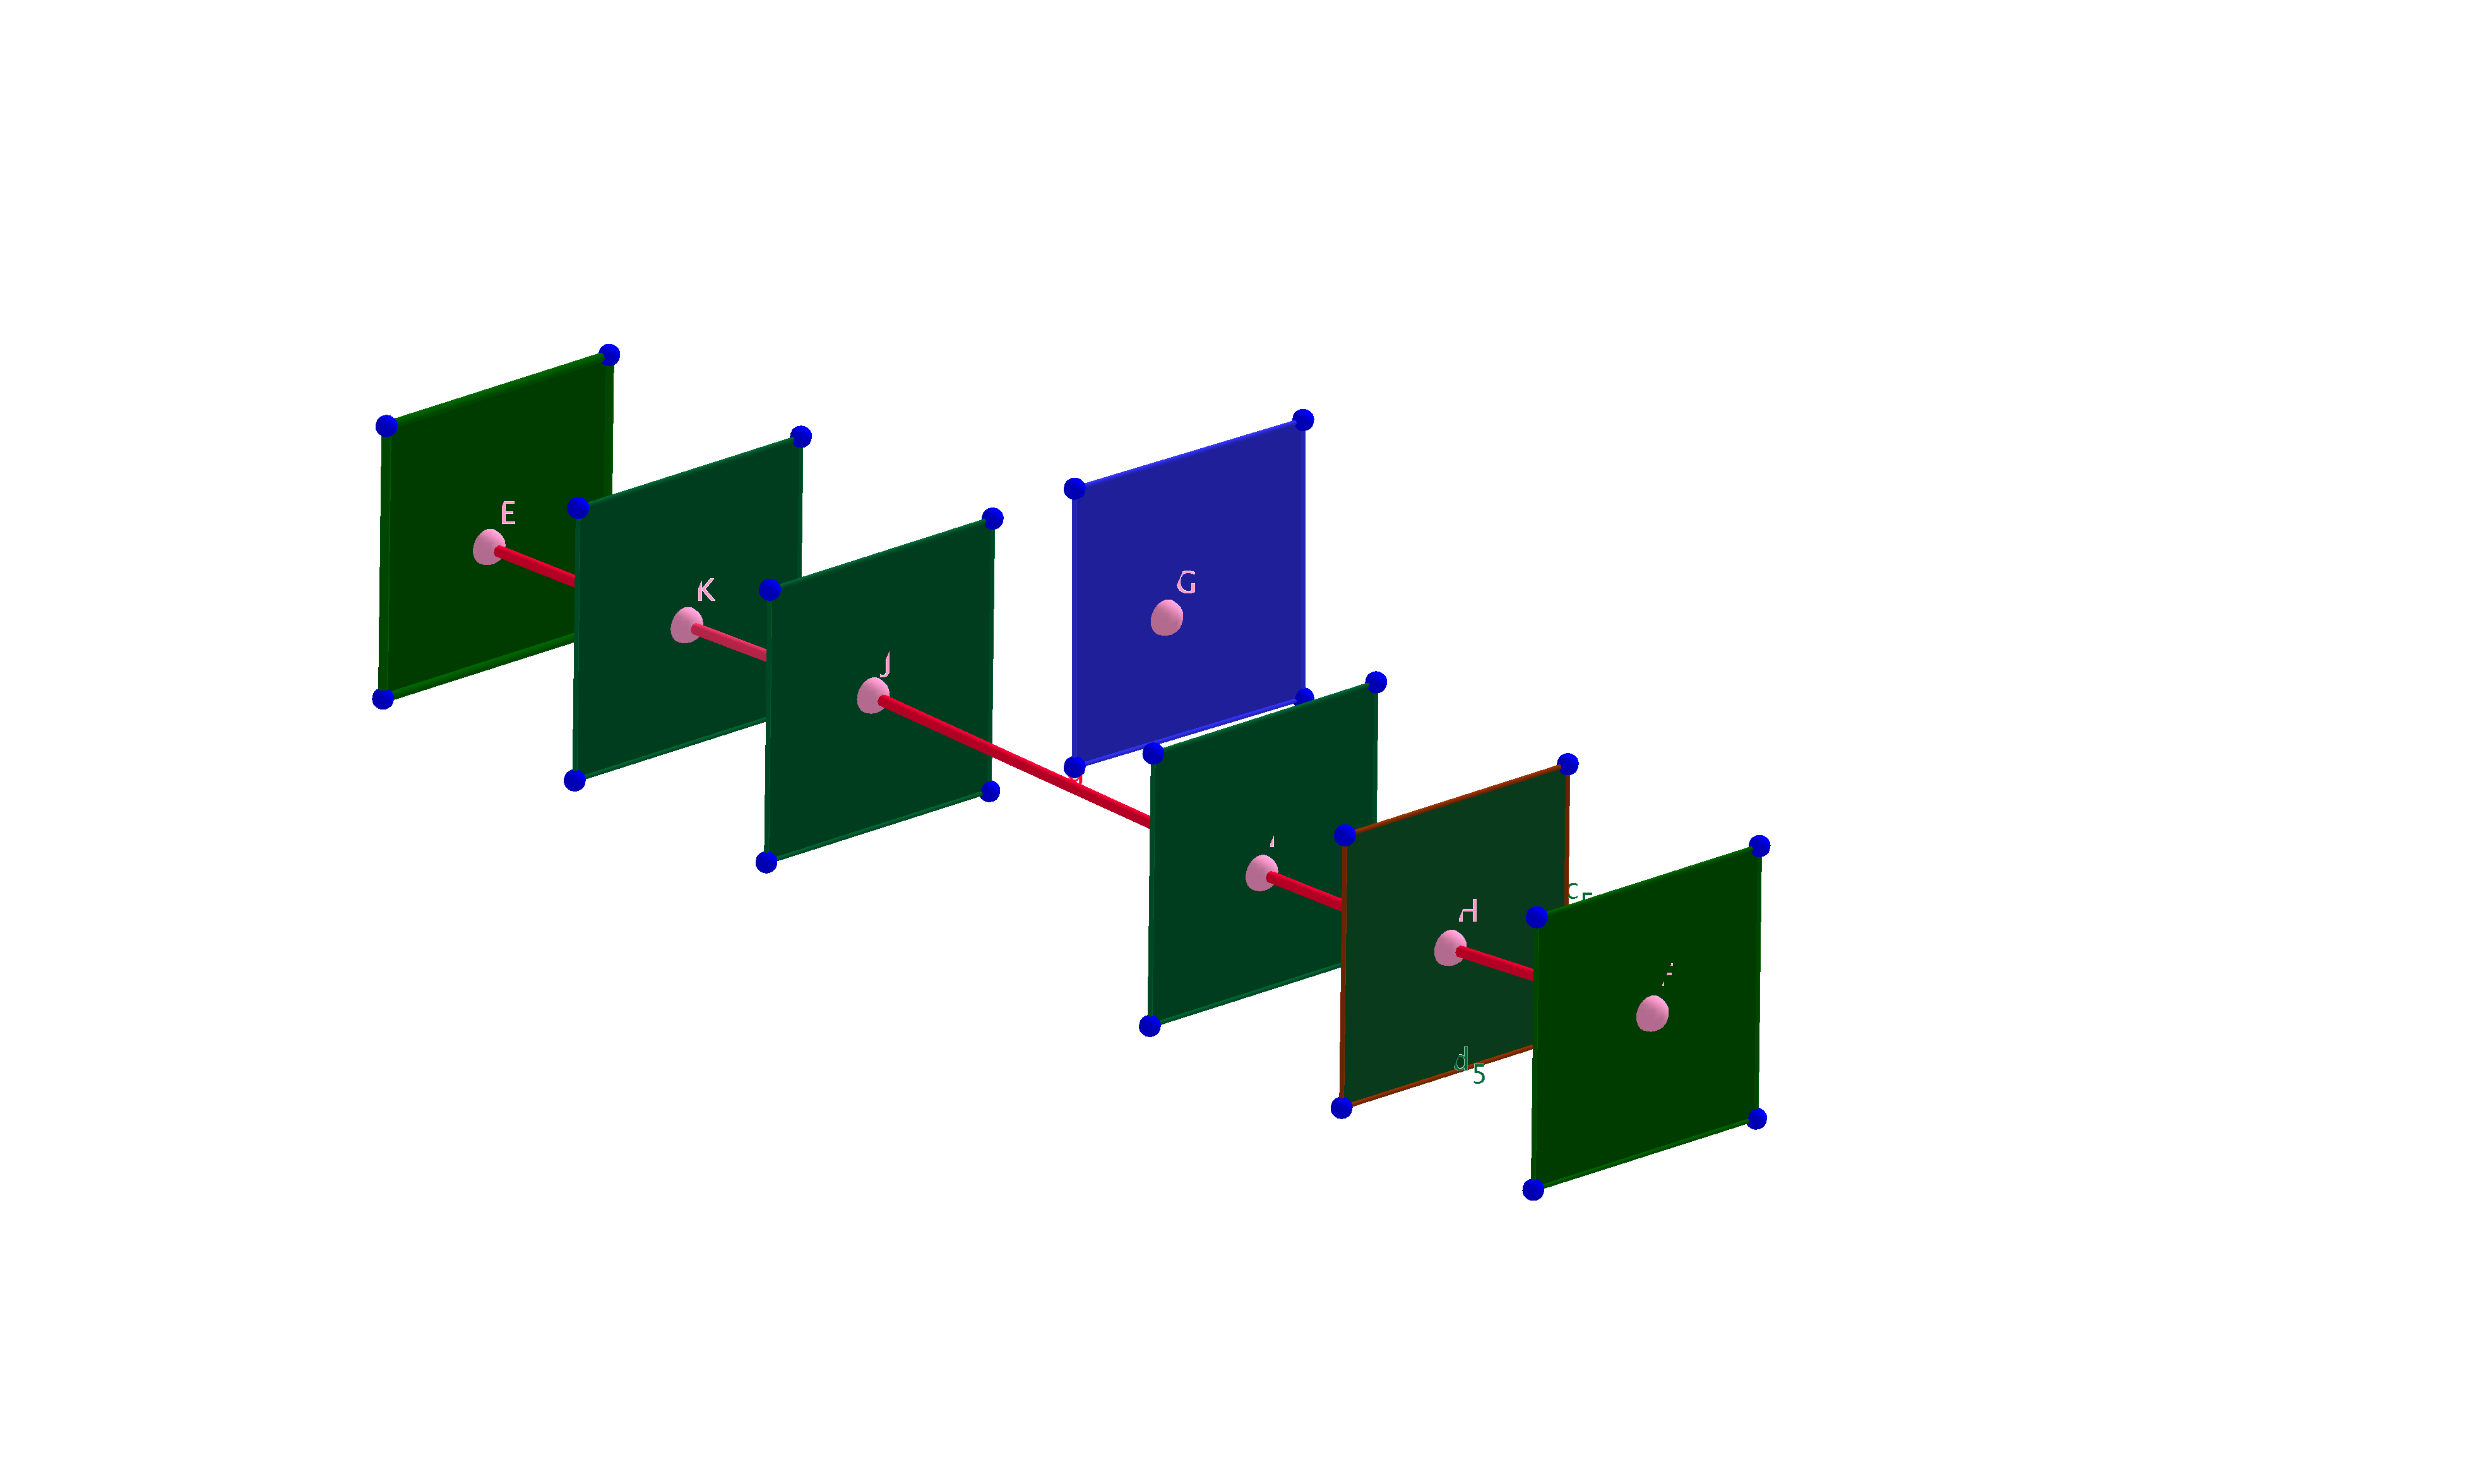
\includegraphics[width=1.0\linewidth]{figures/MisAlignStraight.png}
\caption{Illustration of misalignment with DUT. The transformation of the local DUT frame to the global frame must be wrong so should be corrected.}
\label{fig:MisAlign}
\end{figure}

Figure \ref{fig:MisAlign} illustrates a clear problem with the description of the sensor in space. This is corrected by finding the correction to the transformation between global and local which minimises the residual weighted with errors for all tracks and planes.

A link between the local frame residual and alignment parameters which define the transformations must be determined. The alignment parameters are defined $(X,Y,Z, \alpha,\beta,\gamma)$ which are the offsets in the global frame and the rotations defined in each frame of the rotations applied before it. This last point is important: The corrections to the rotations must be determined in the frame reached before that rotation is applied. So the $R_X$ (Rotation round X axis) matrix correction must be determined after you have rotated round the Z axis. This can be dealt with in two ways: 

1) Determine the corrections for each rotation in the frame it is applied then rotate to the local frame. 

2) Only apply large rotations and parity transforms before you apply corrections. 

The second approach is taken with all X/Y rotations applied in the initial rotation matrix. Note rotation round the Z axis is also permissible since this is the first matrix to be corrected. The parameters' change is related to change in position of a point in the coordinate system by the  \emph{point correction matrix} $\hat{PC}(X,Y,Z, \alpha,\beta,\gamma)$:
\[ \left( \begin{array}{cccccc}
1 & 0 & 0 & 0 & relZ & -relY \\
0 & 1 & 0 & -relZ & 0 & relX  \\
0 & 0 & 1 & relY & -relX & 0   
  \label{eq:PC}
\end{array}
 \right)\] 

This matrix will create a correction vector at the location and coordinate system specified by the relative positions. 
The relative positions are defined as the global predicted position without offsets. This is done so the order of magnitude of the rotation is correct. So defined as:

\begin{equation}
 \overrightarrow{rel} =   \hat{R}\overrightarrow{L} 
\end{equation}

The predicted positions used are the pattern recognition tracks and not the GBL fit.  

\begin{figure}[H]
\centering
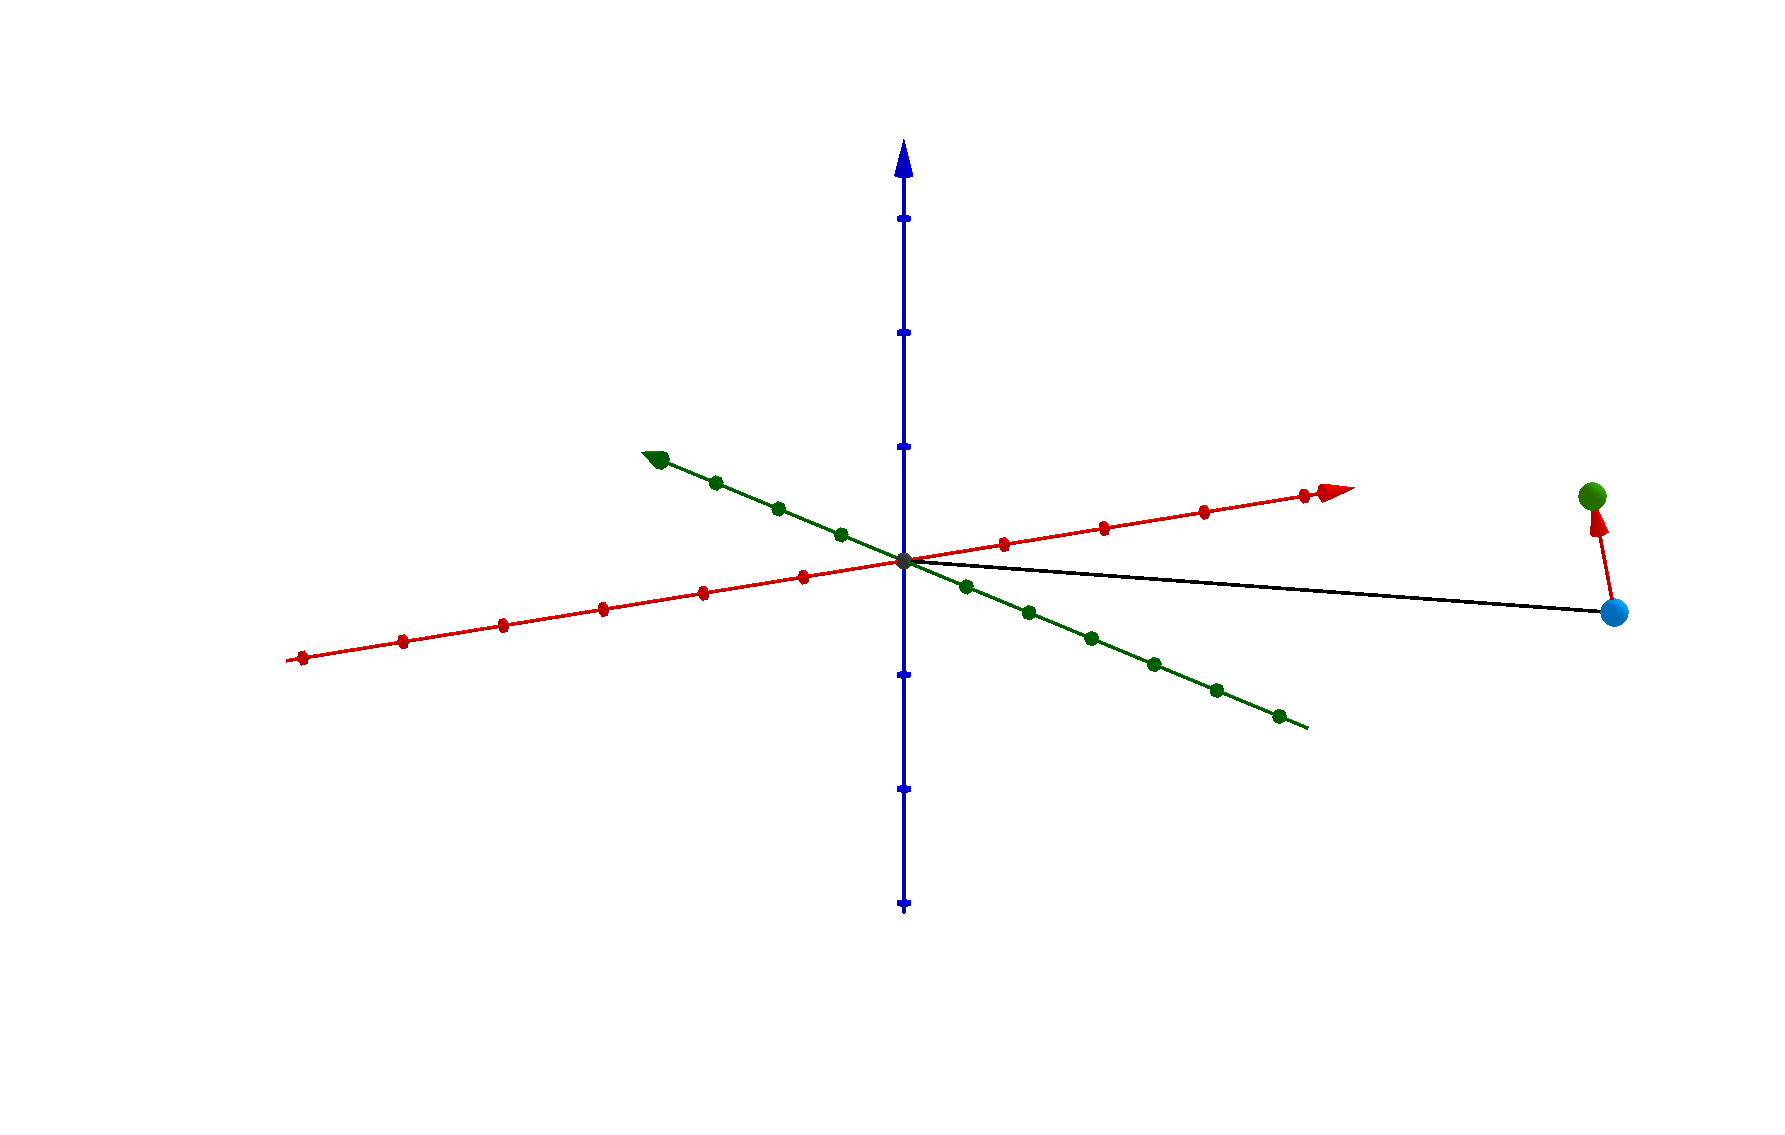
\includegraphics[width=1.0\linewidth]{figures/corrAlign.png}
\caption{The point correction matrix for a particular relative positions. The vector is the correction to apply to this point given a certain $(X,Y,Z, \alpha,\beta,\gamma)$ change in the coordinate system.}
\label{fig:CorrMatrix}
\end{figure}

The correction vector will not give the change measured on the plane from moving the track. To estimate this the correction vector must be considered moving a track rather than a point. This is done using the \emph{track correction matrix} $\hat{TC}(\overrightarrow d, \overrightarrow n )$ of the from.
\begin{equation}
  I -  \frac{\overrightarrow d \times \overrightarrow n}{\overrightarrow d . \overrightarrow n}\\
  \label{eq:TC}
\end{equation}

which will move a track by a particular displacement and determine how this changes the intersection with a plane. 

\begin{figure}[H]
\centering
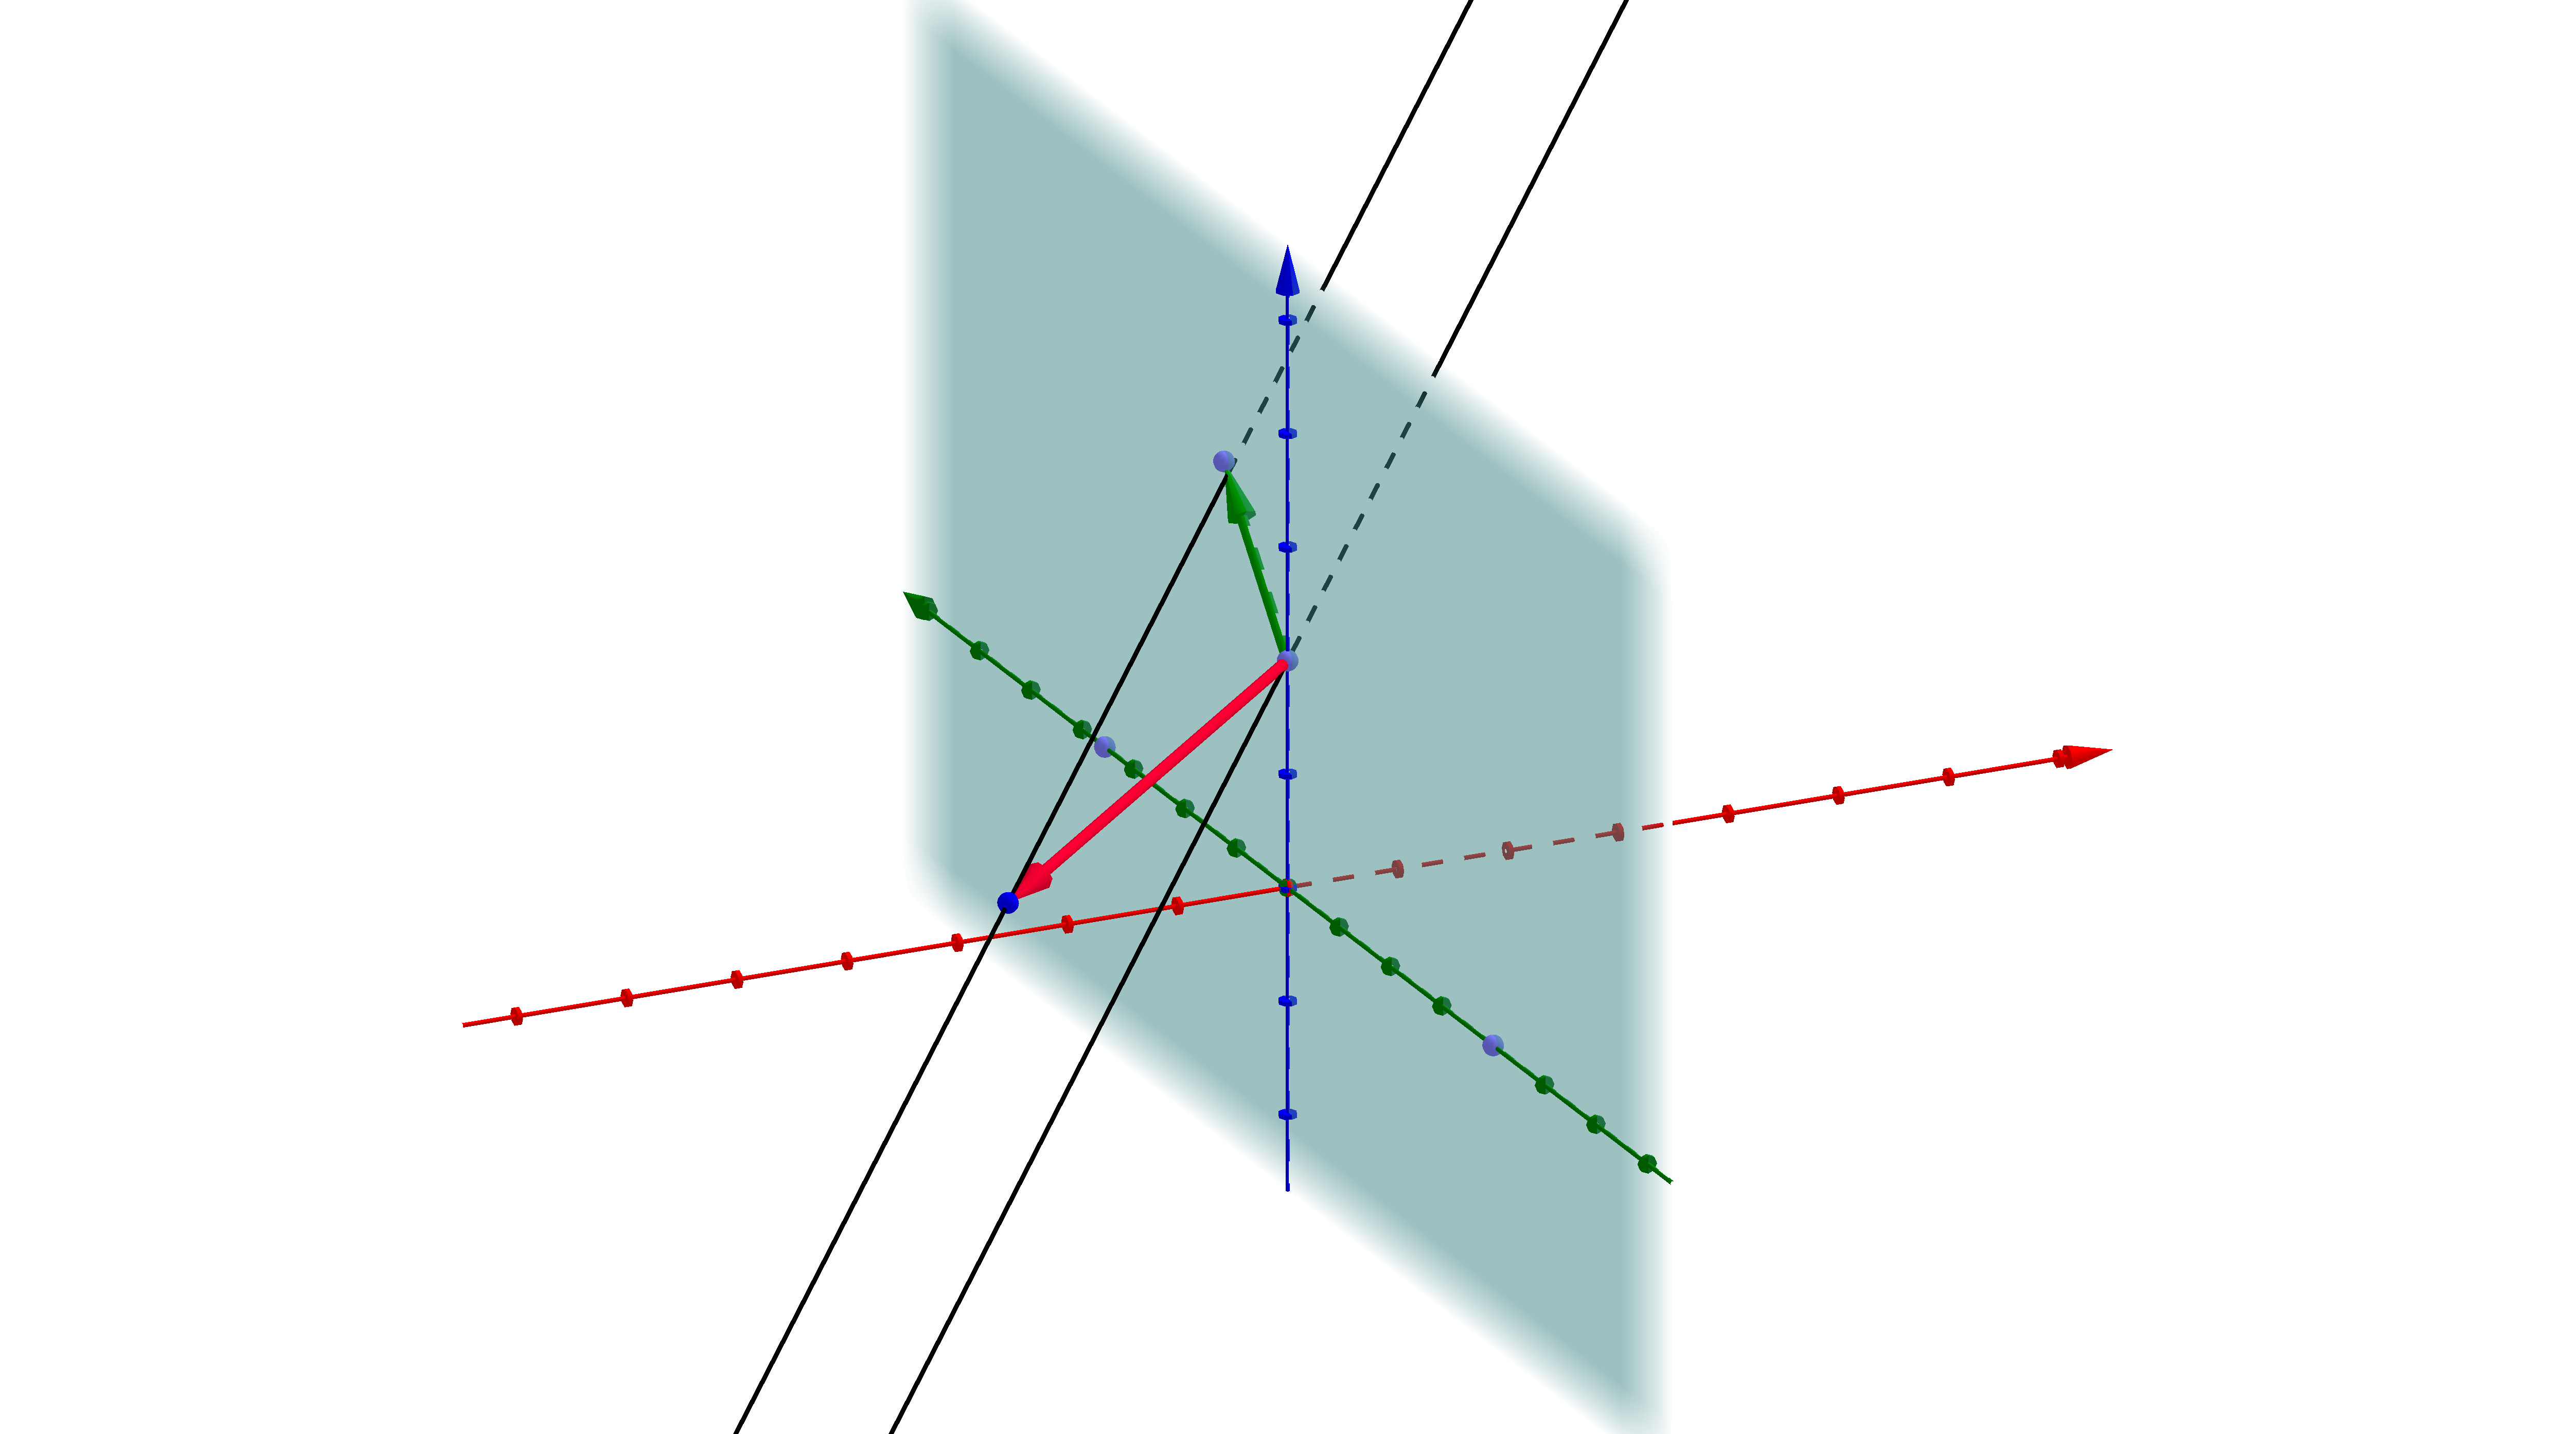
\includegraphics[width=1.0\linewidth]{figures/alignBigger.png}
\caption{The track correction matrix will take as input the track displacement given in red. It will then determine the green vector which is the change on the plane due to that displacement}
\label{fig:TC1}
\end{figure}

\begin{figure}[H]
\centering
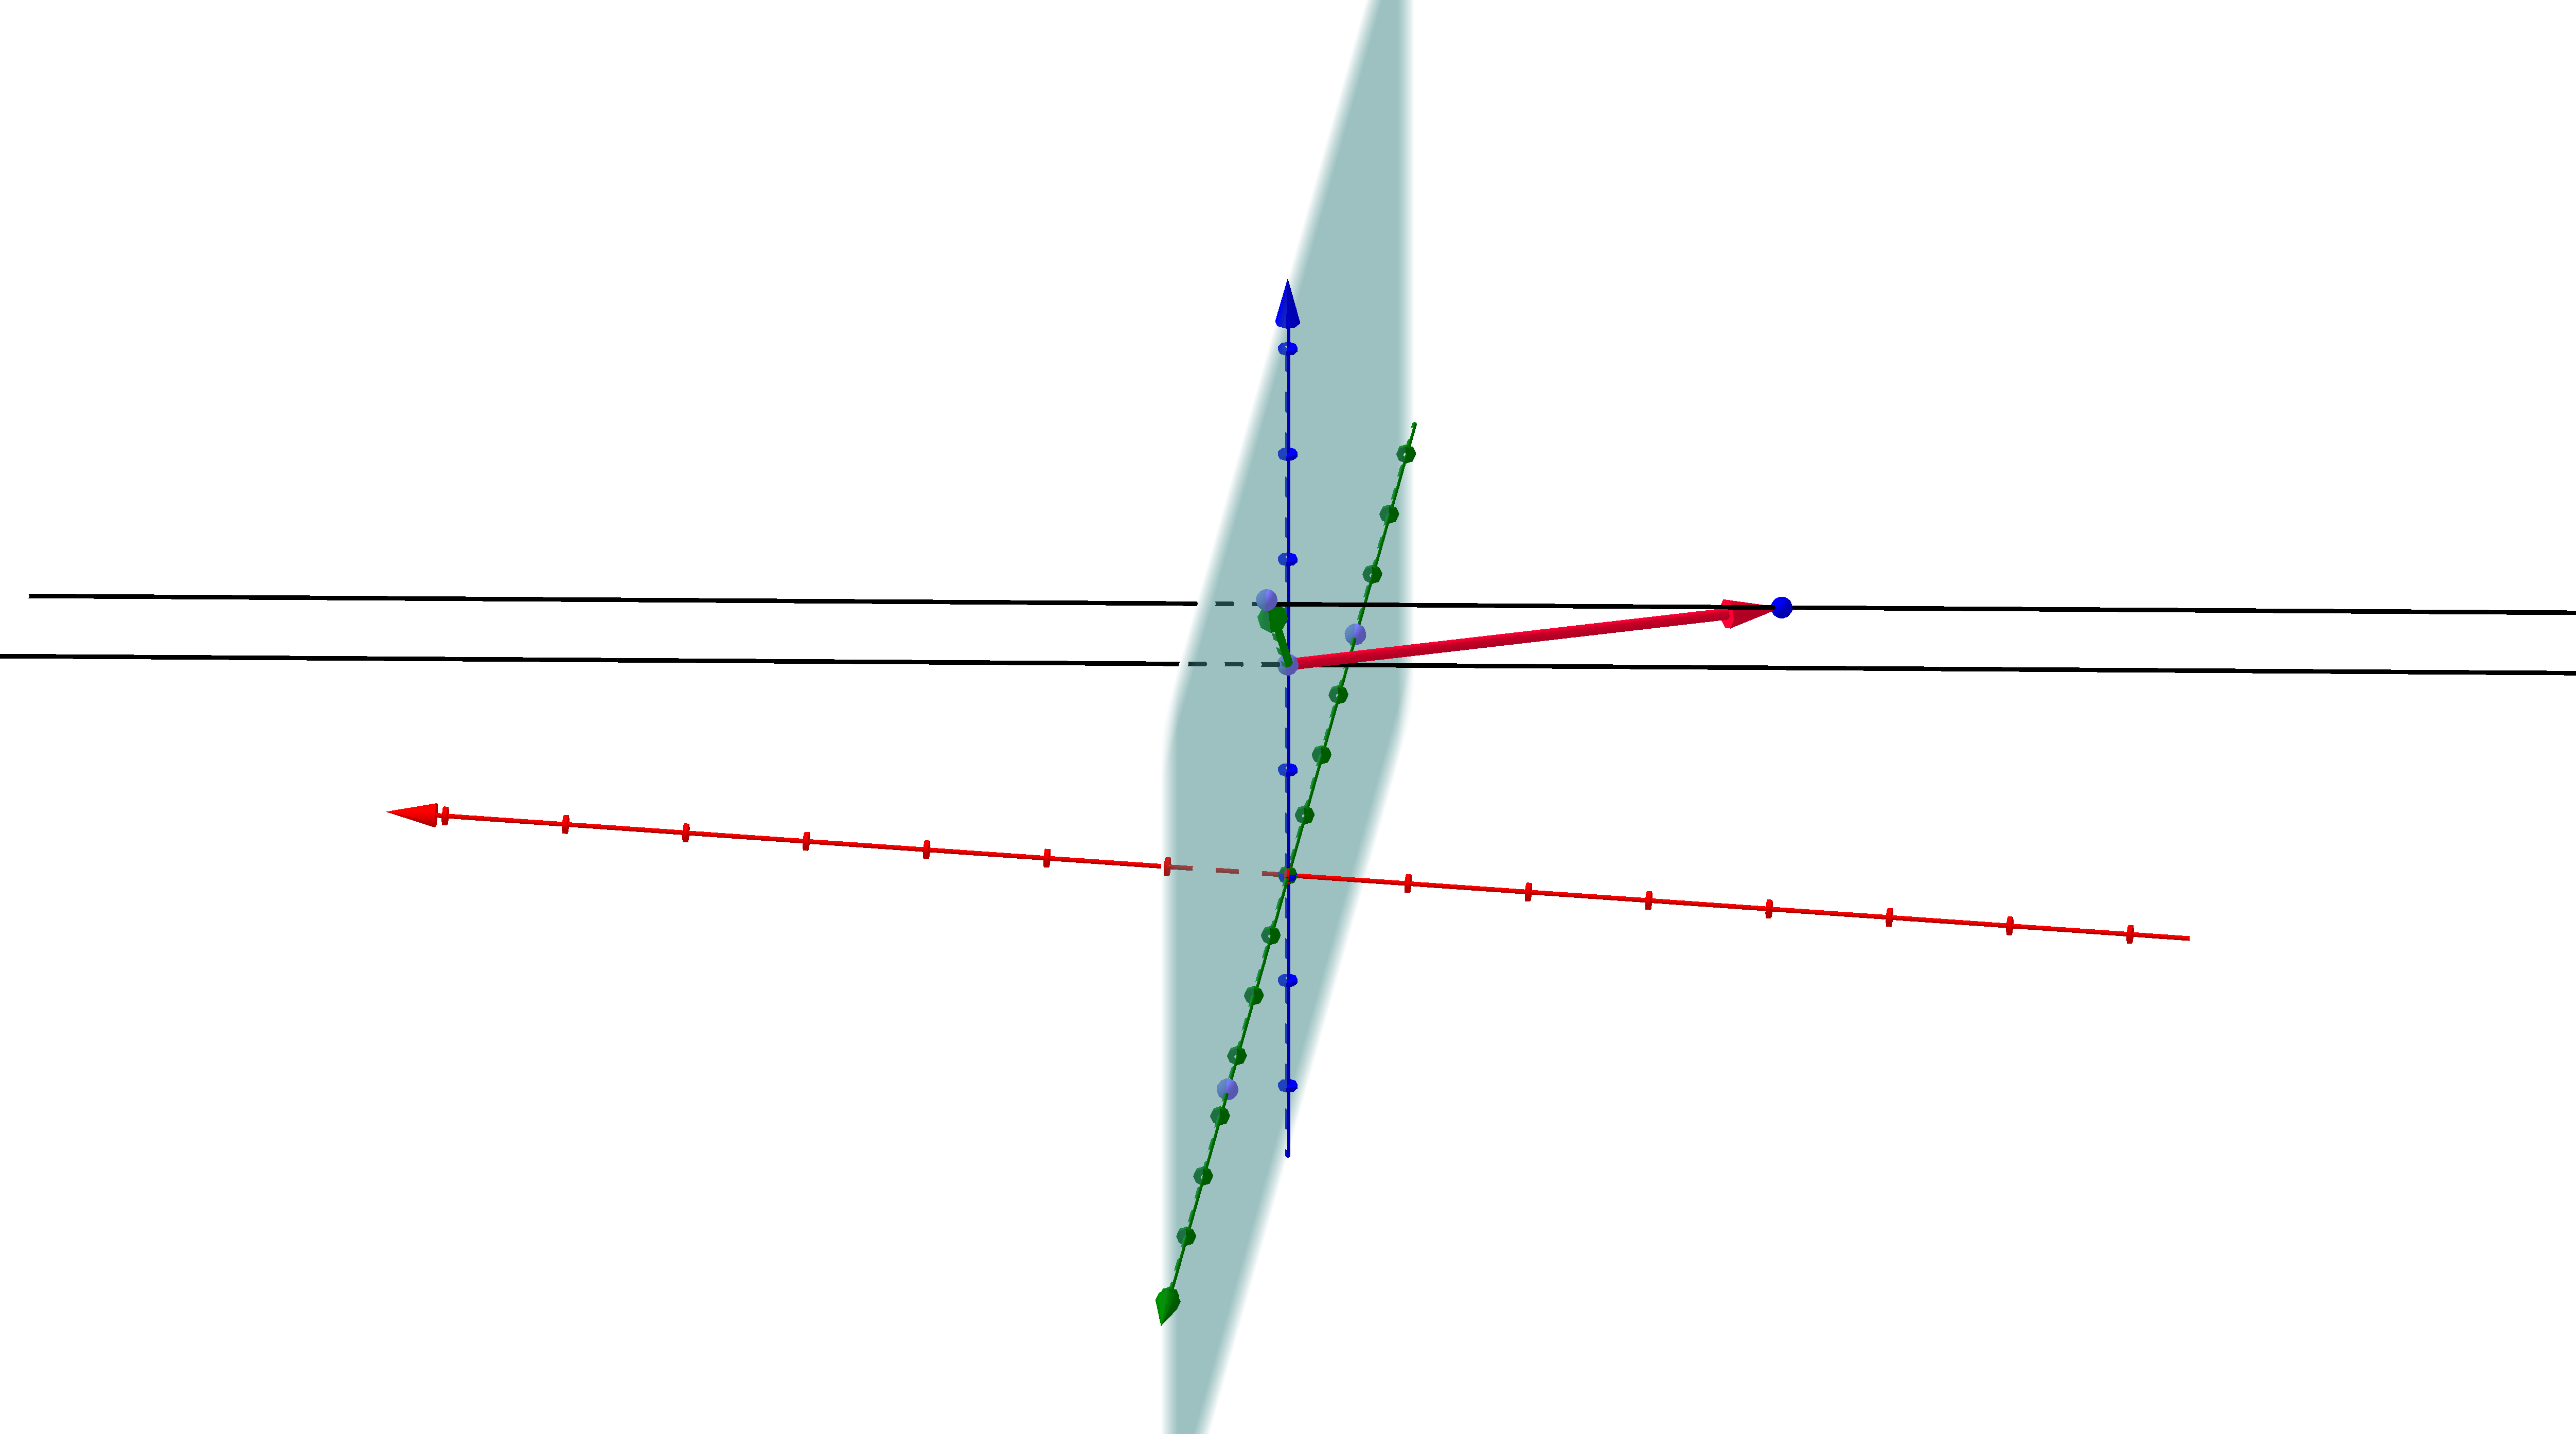
\includegraphics[width=1.0\linewidth]{figures/alignmentBigger.png}
\caption{Same as \ref{fig:TC1} but from a different angle. The green vector is on the plane surface.}
\label{fig:TC2}
\end{figure}

The final full body alignment can determined by combining TC and PC. This will relate the change in global alignment parameters to change on a plane. The plane described is in the global frame. Therefore the vector on the plane must be rotated into the local frame of the sensor. This frame will of course have zero Z displacement since it should be on the sensor surface. The final matrix passed to millepede:

\begin{equation}
\hat{R^{T}} \hat{TC} \hat{PC} 
\end{equation}

\subsection{Add local parameters}

\newpage

\section{Examples}

Examples which are installed with EUTelescope can be run from installation. The only additional requirement is you have access to DESY afs. A brief outline of some examples with be given below to show what can be done with the fitter. All examples in jobsub/examples/GBL directory in EUTelescope. A step by step guide of what parameters to change in the config is given in the README for each example. All histograms with DUT residual is without the DUT included in the fit.

\subsection{Quad}

\begin{figure}[H]
\hspace{-35mm}
\subfloat{\label{fig:beamE5B1} 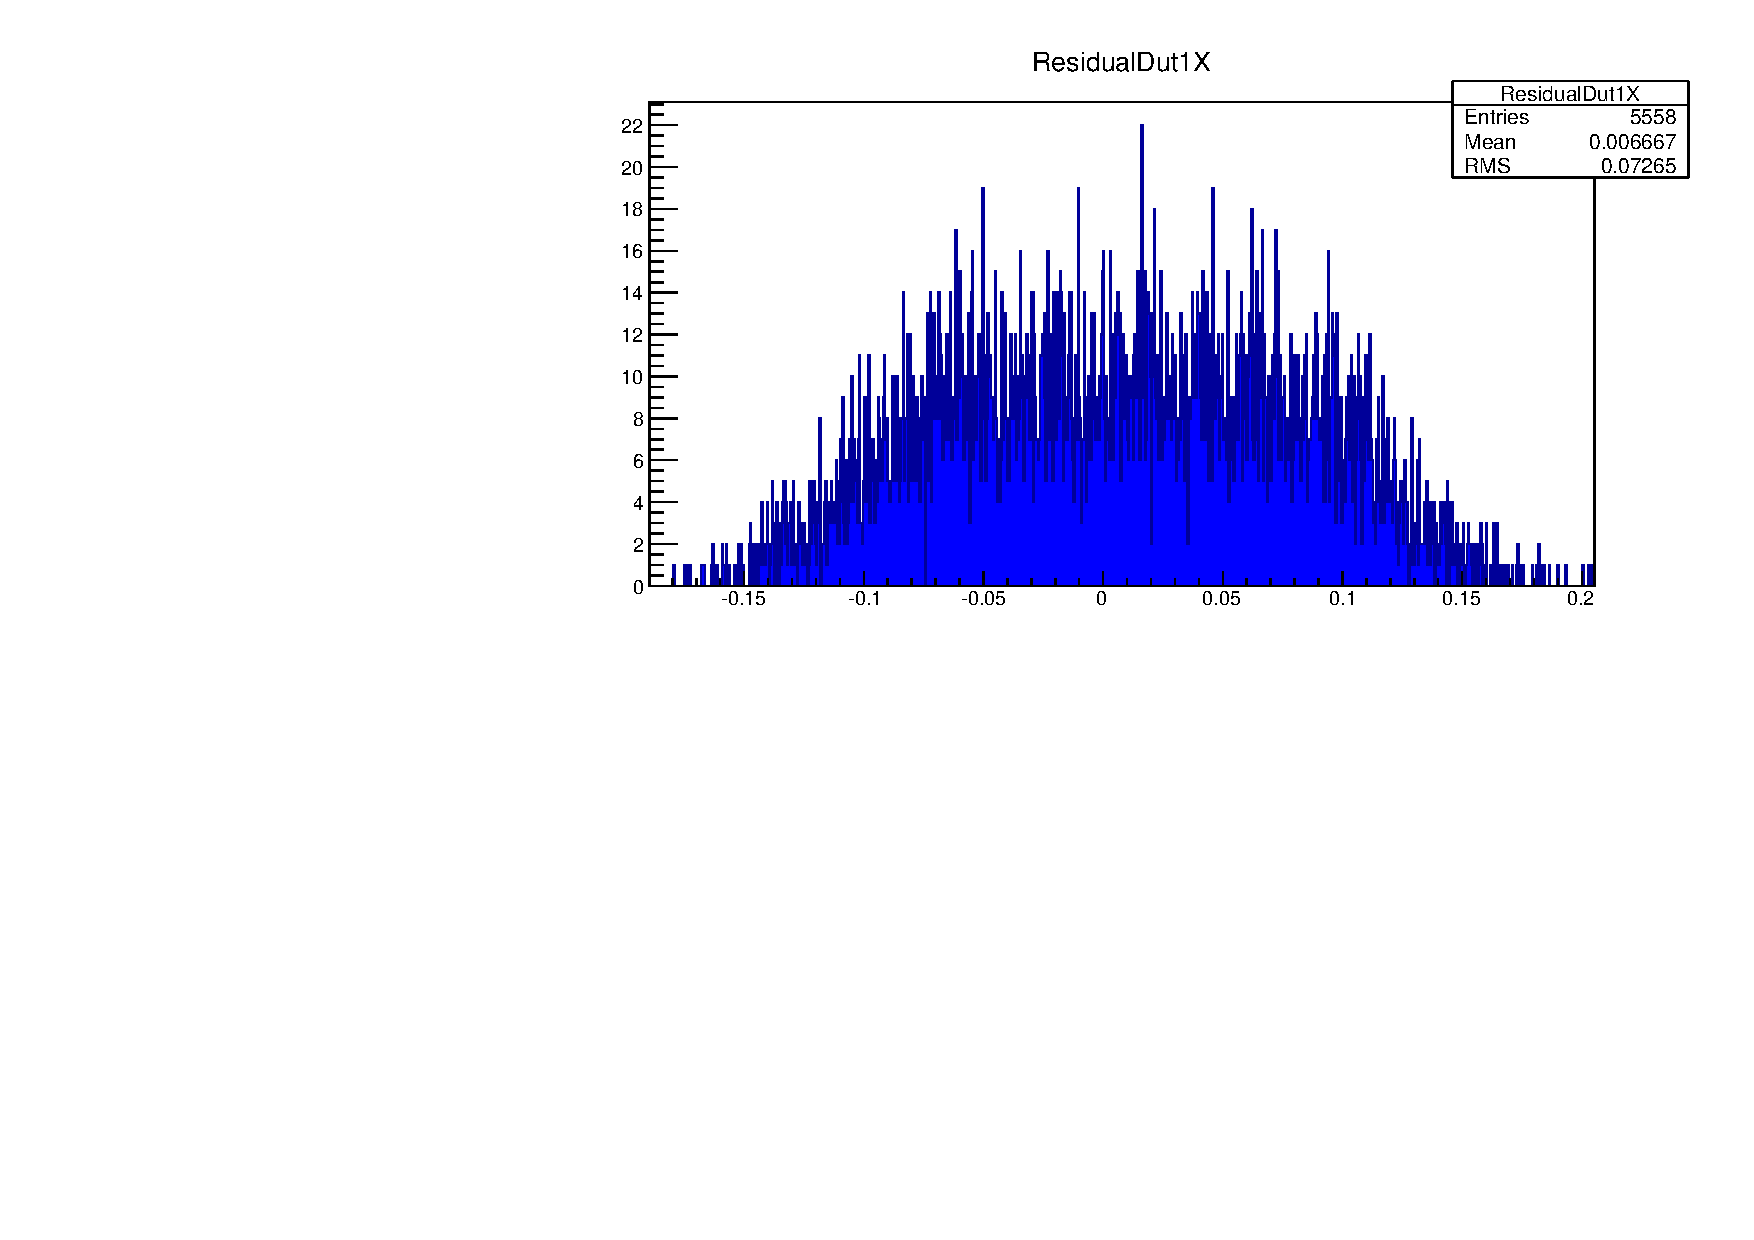
\includegraphics[scale=0.5]{figures/QuadXRes21.pdf}}
\subfloat{\label{fig:beamE5B1} 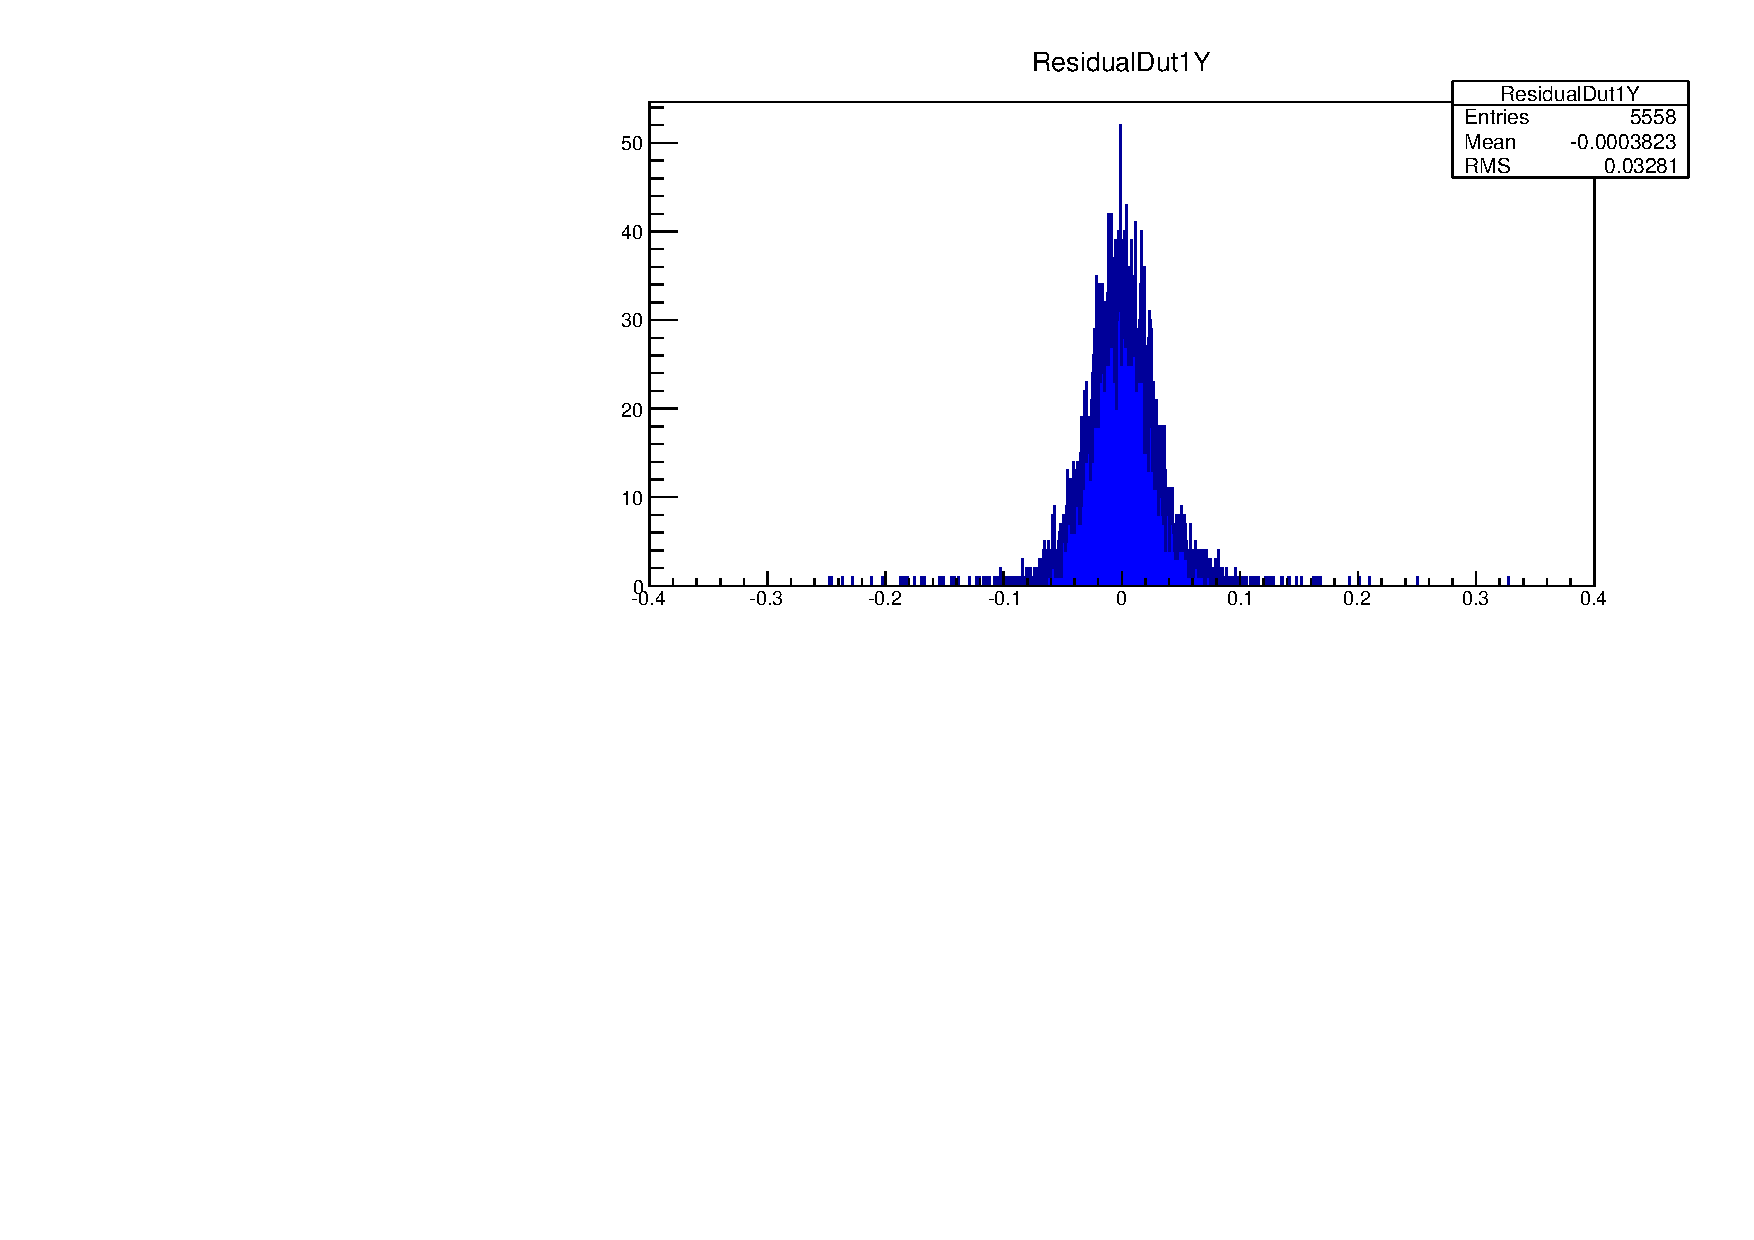
\includegraphics[scale=0.5]{figures/QuadResY.pdf}}
\caption{ Residual of Quad module in local X/Y axis. }
\label{fig:chiRad}
\end{figure}

\subsection{APIX pixel}

\begin{figure}[H]
\hspace{-35mm}
\subfloat{\label{fig:beamE5B1} 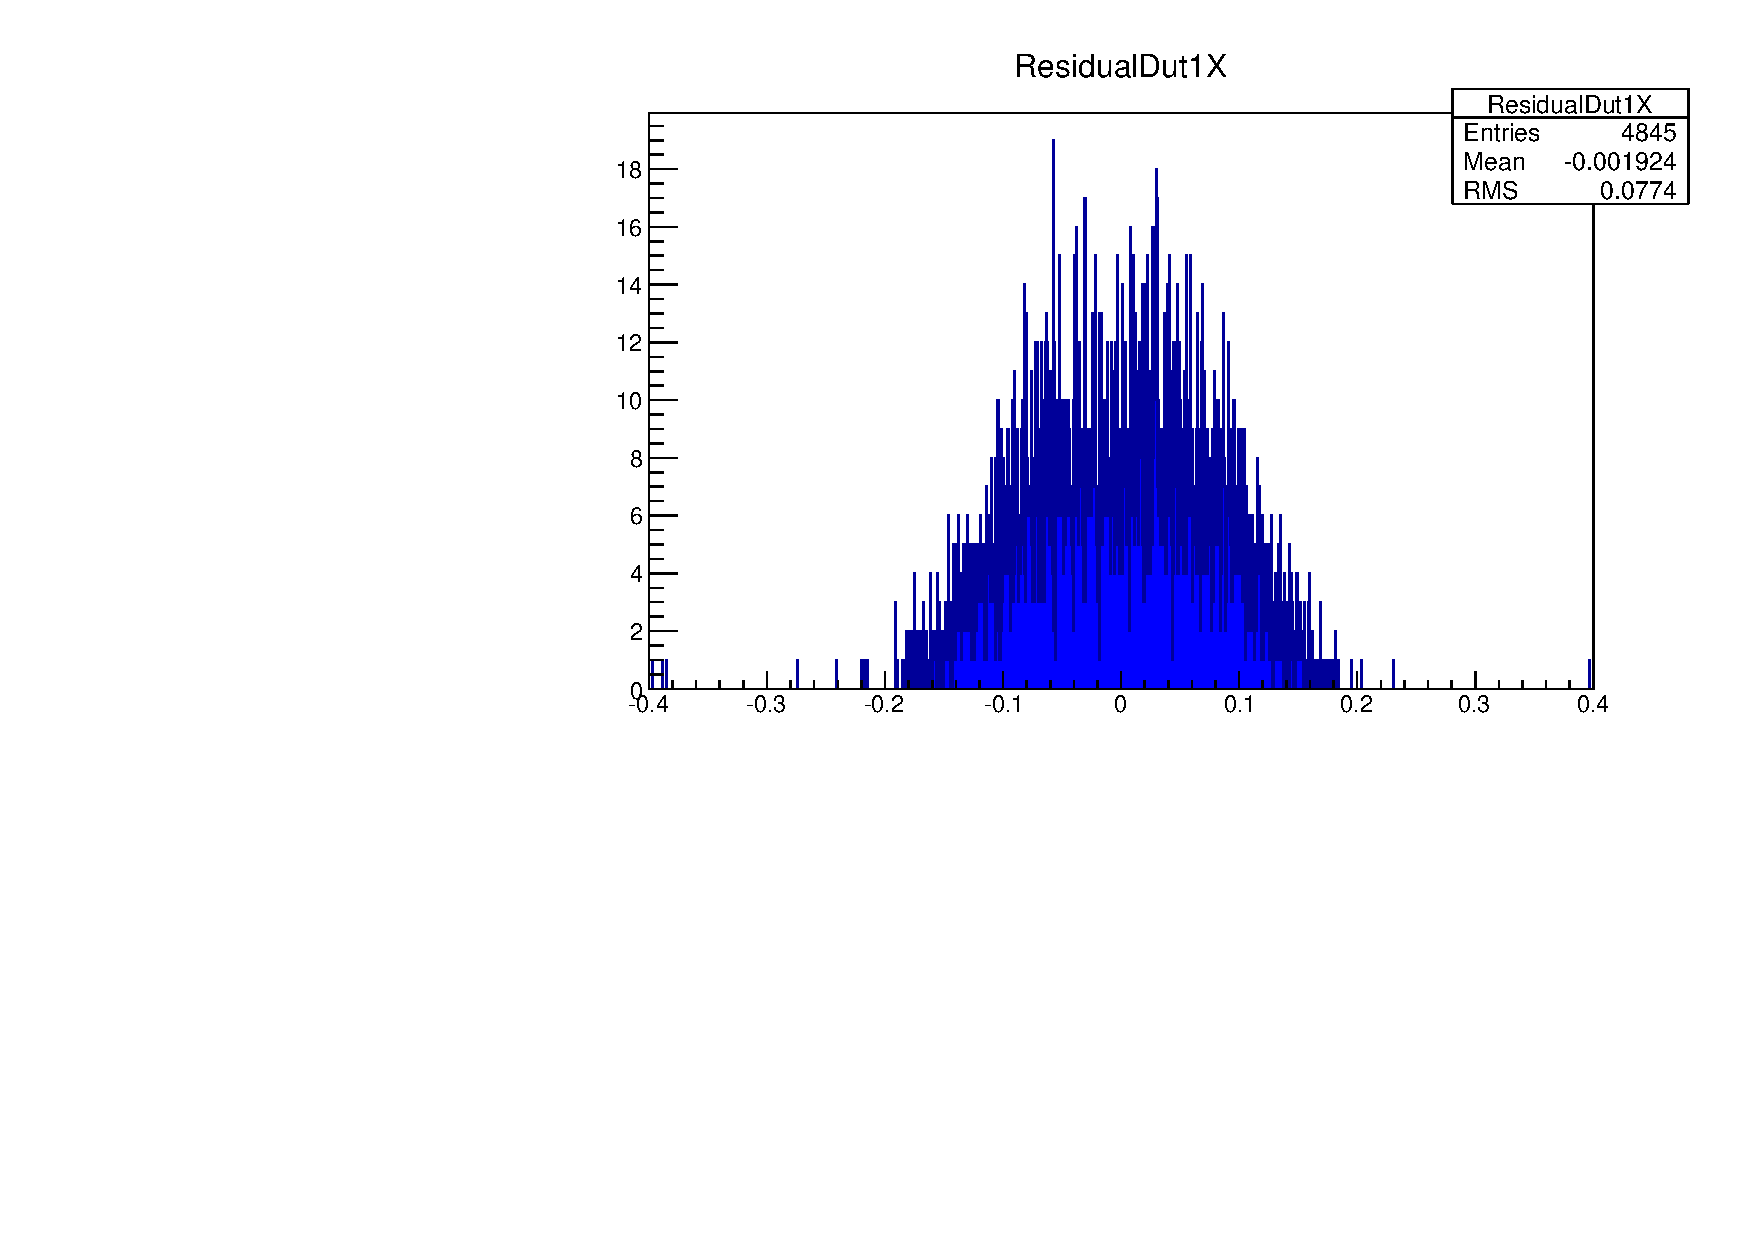
\includegraphics[scale=0.5]{figures/resXpixel.pdf}}
\subfloat{\label{fig:beamE5B1} 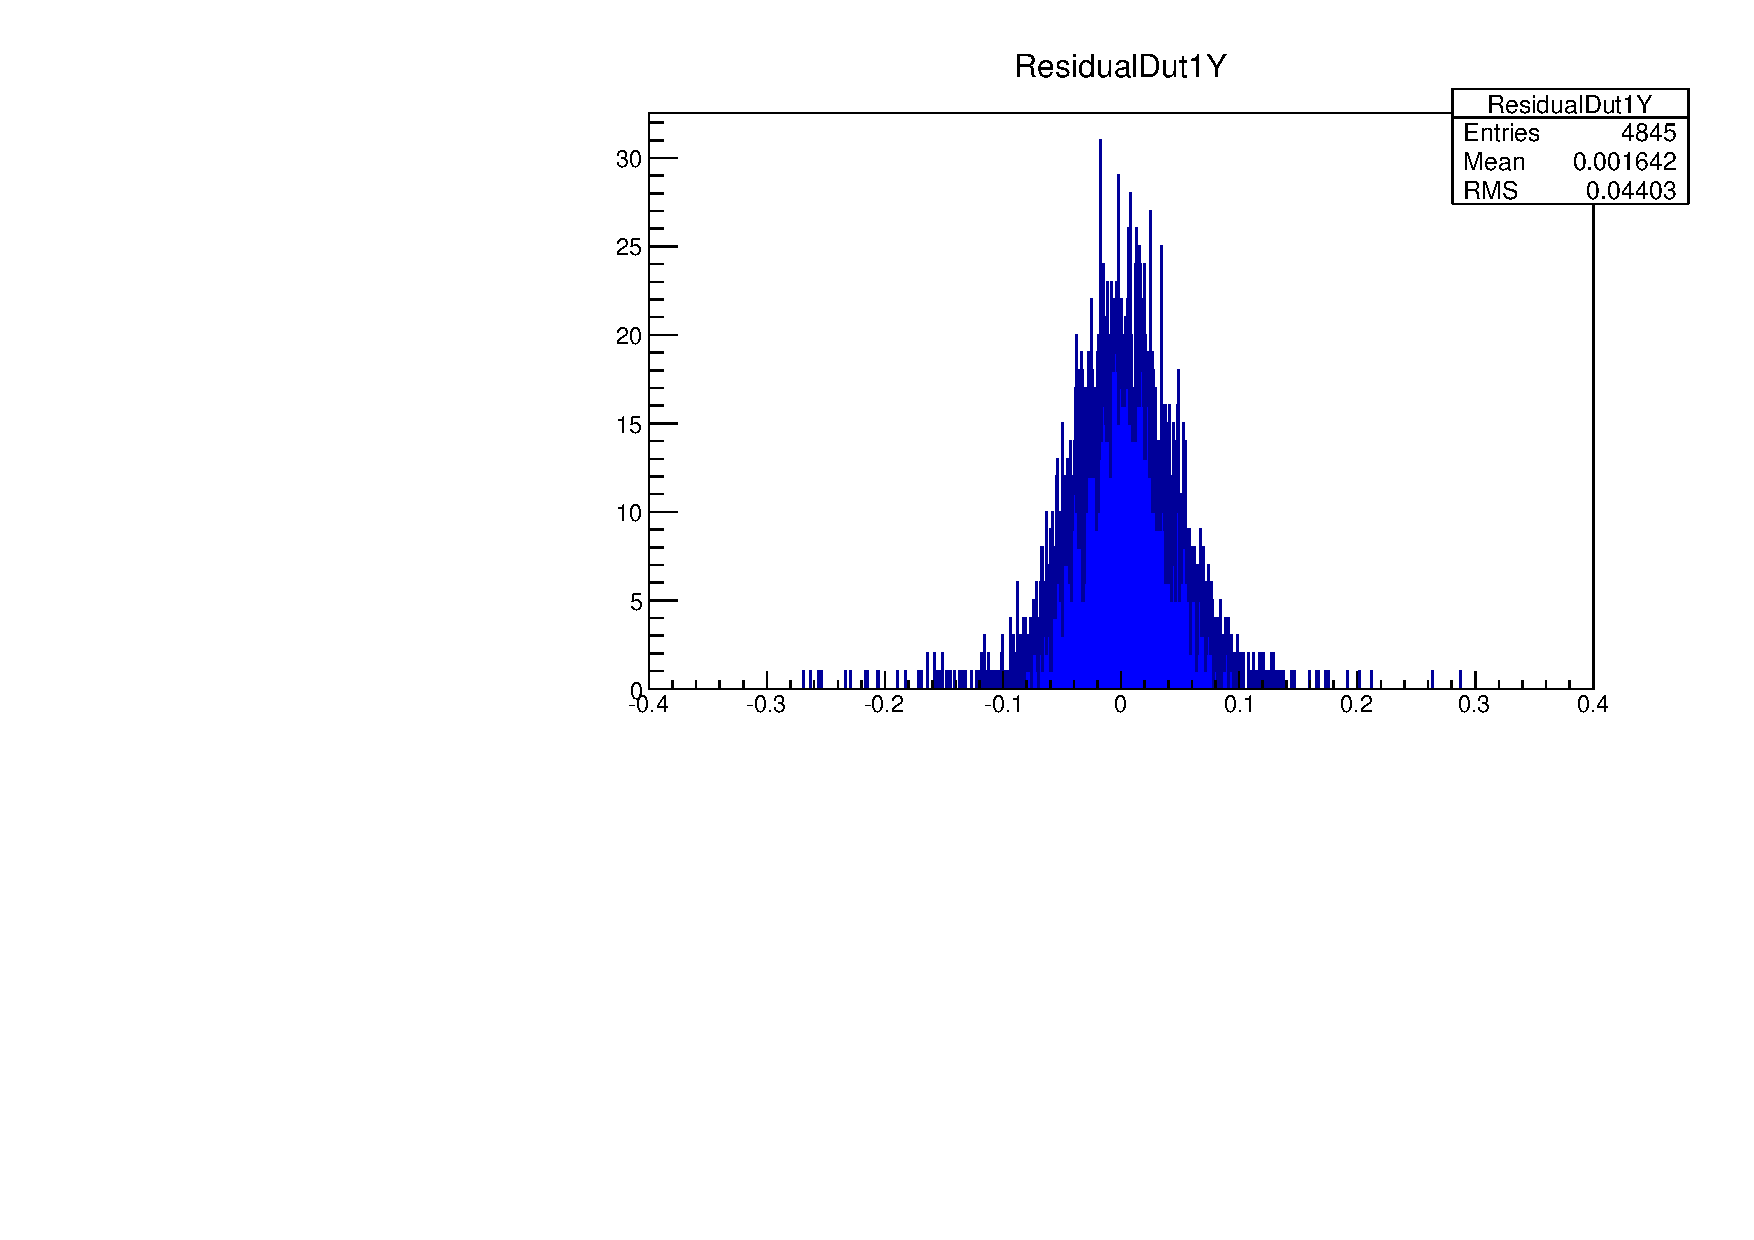
\includegraphics[scale=0.5]{figures/resYpixel.pdf}}
\caption{The resolution with 10k events on DUT 21. }
\label{fig:kinkRad}
\end{figure}


\begin{figure}[H]
\hspace{-35mm}
\subfloat{\label{fig:beamE5B1} 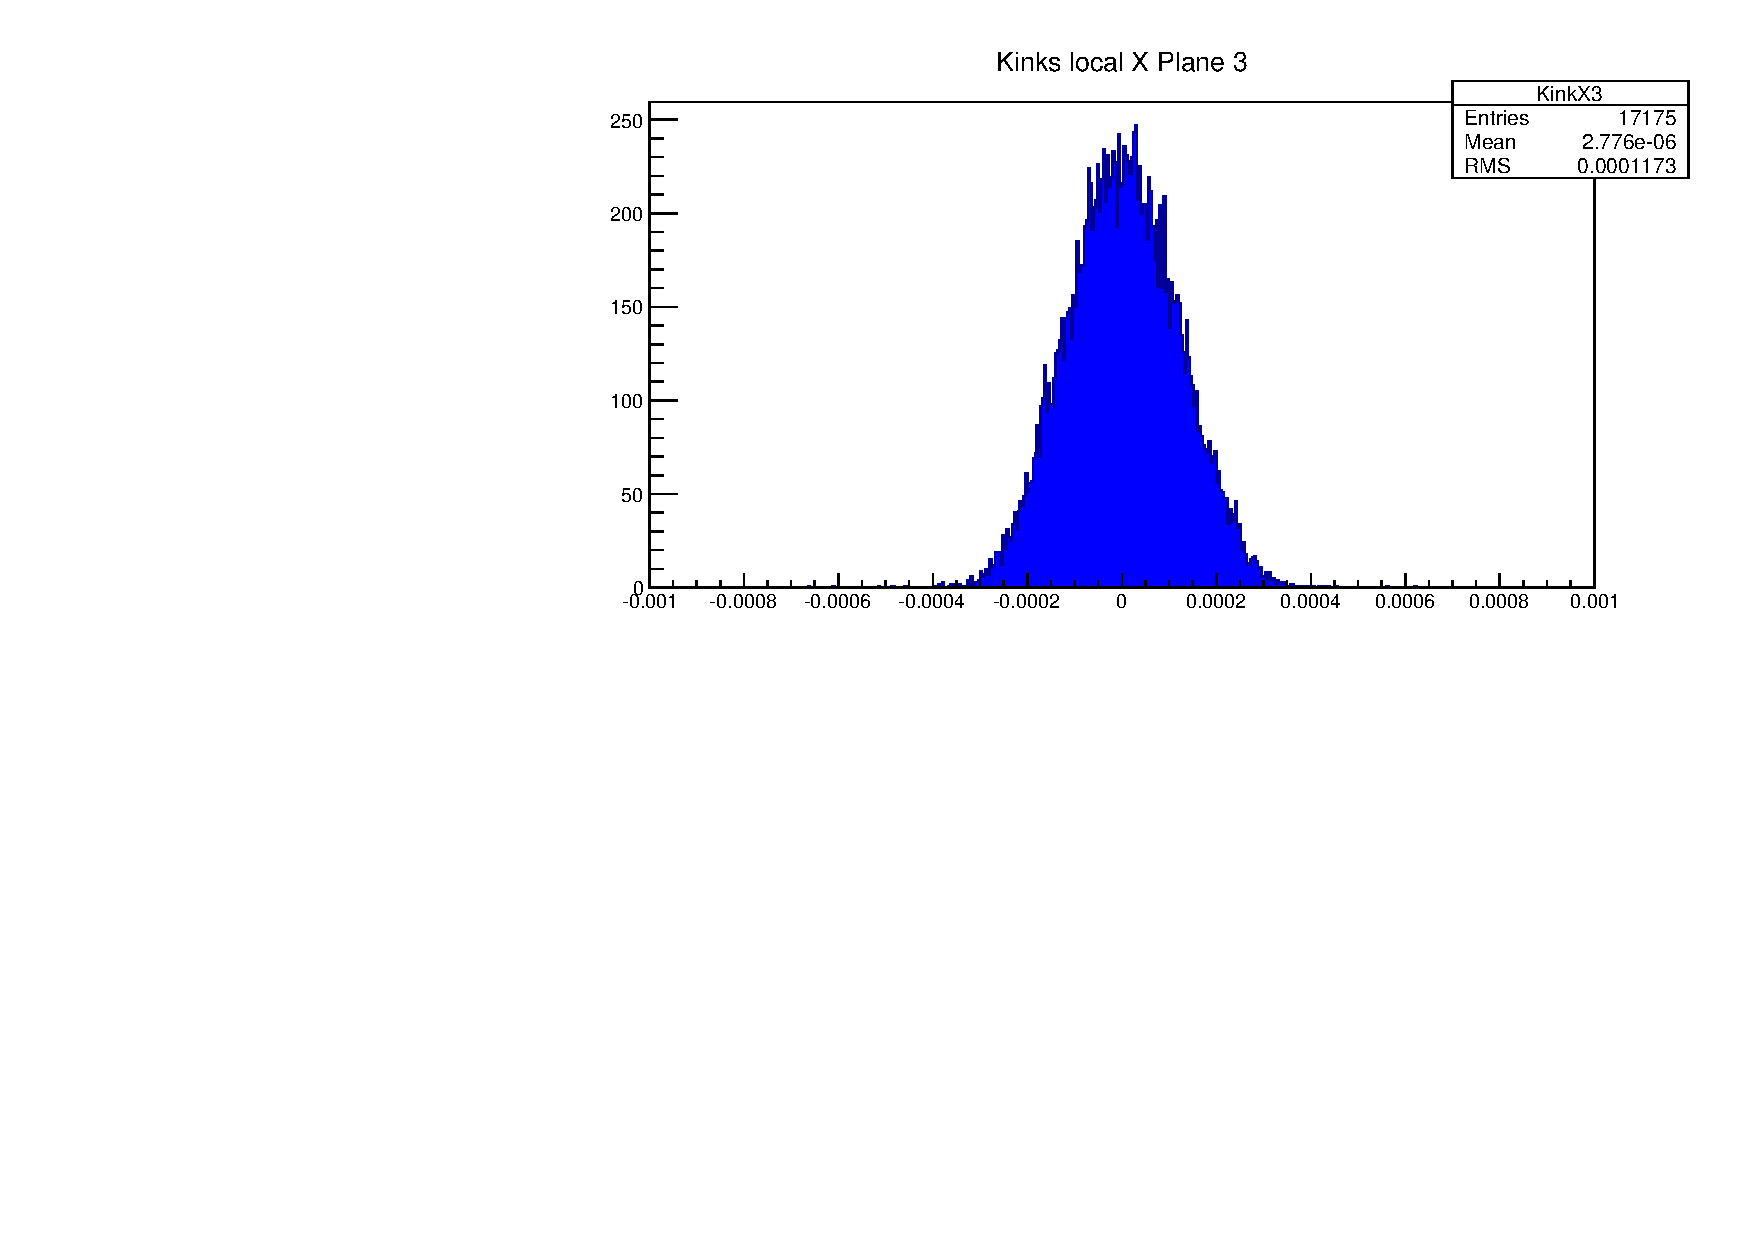
\includegraphics[scale=0.5]{figures/KinkX3Local-313-Wrong.pdf}}
\subfloat{\label{fig:beamE5B1} 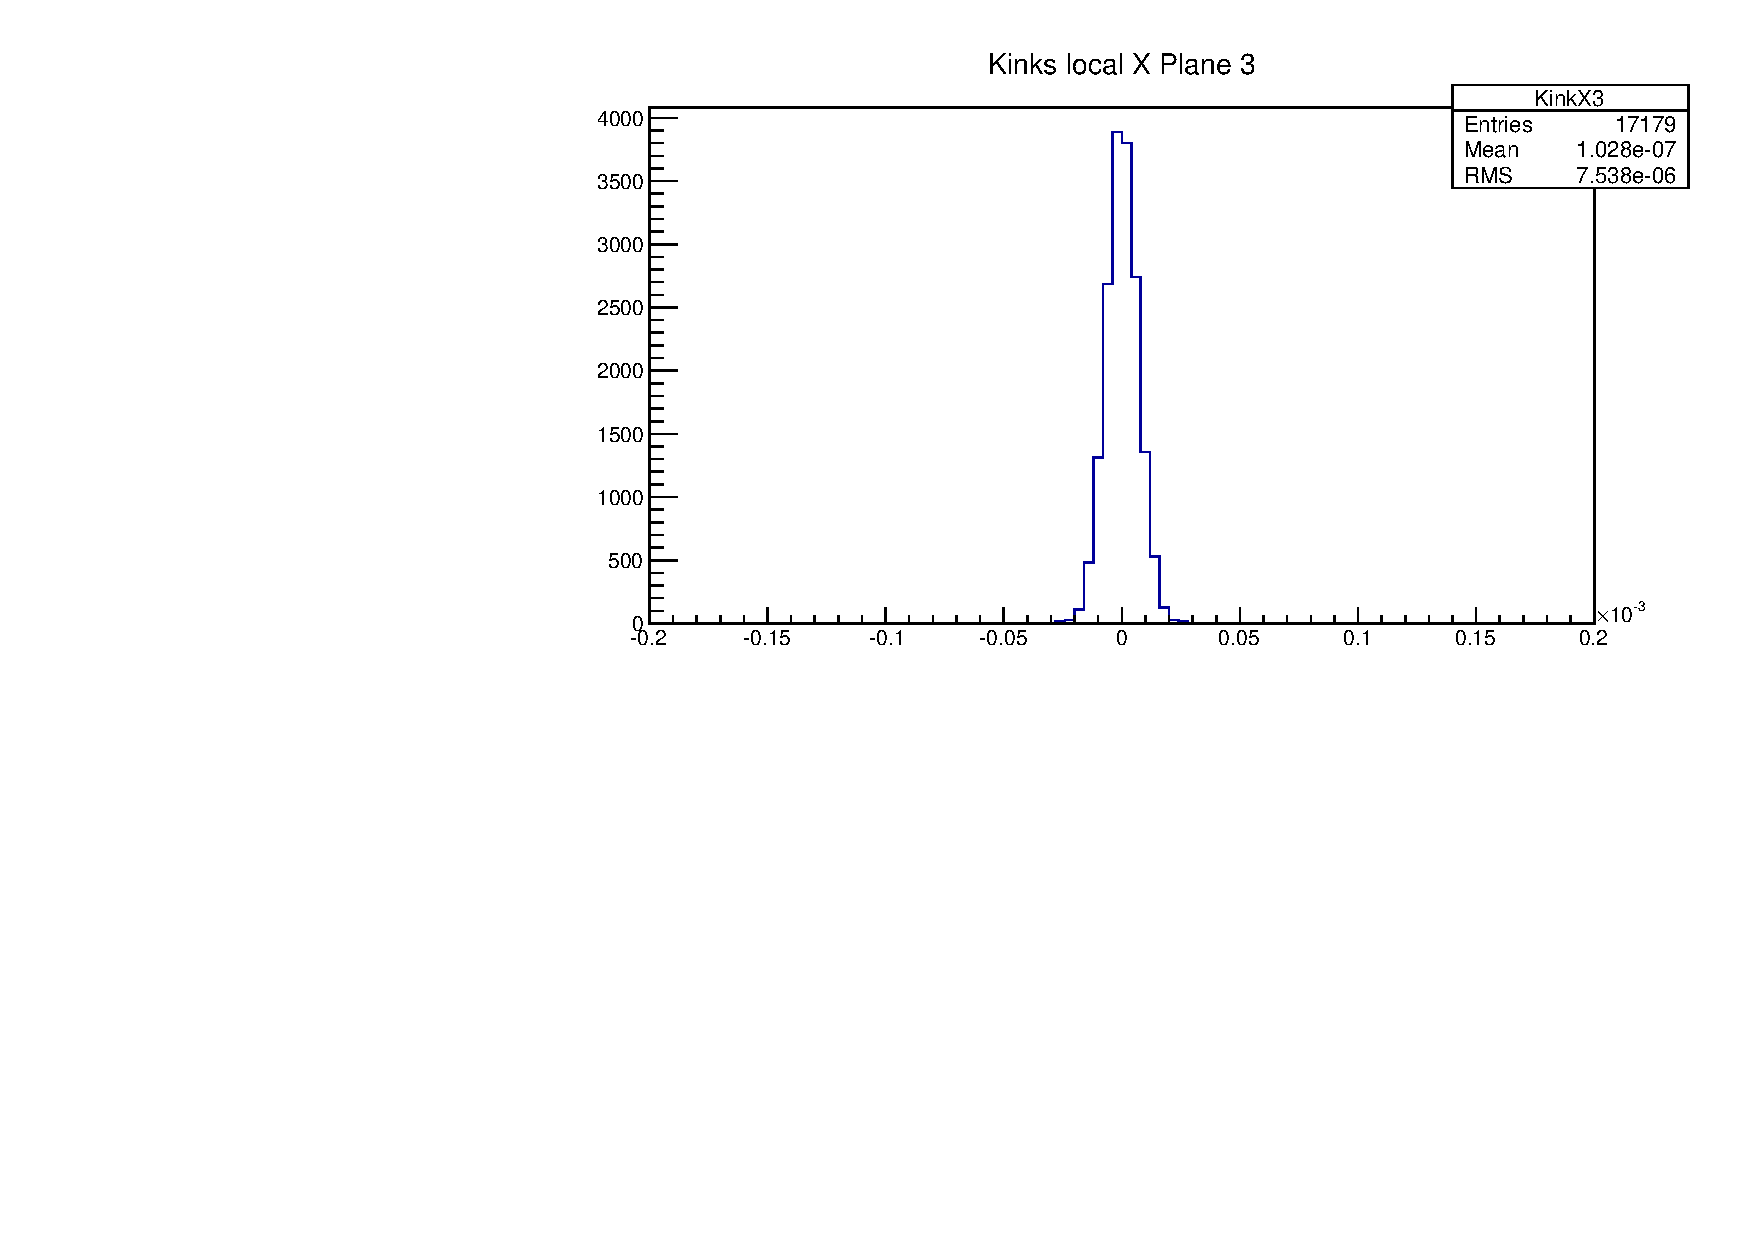
\includegraphics[scale=0.5]{figures/KinkX3Local-313-Corr.pdf}}
\caption{The kink angles for both descriptions. The left has much larger kinks since this has not been incorporated into the scattering}
\label{fig:kinkRad}
\end{figure}

\subsection{APIX mapping}

\begin{figure}[H]
\hspace{-35mm}
\subfloat{\label{fig:beamE5B1} 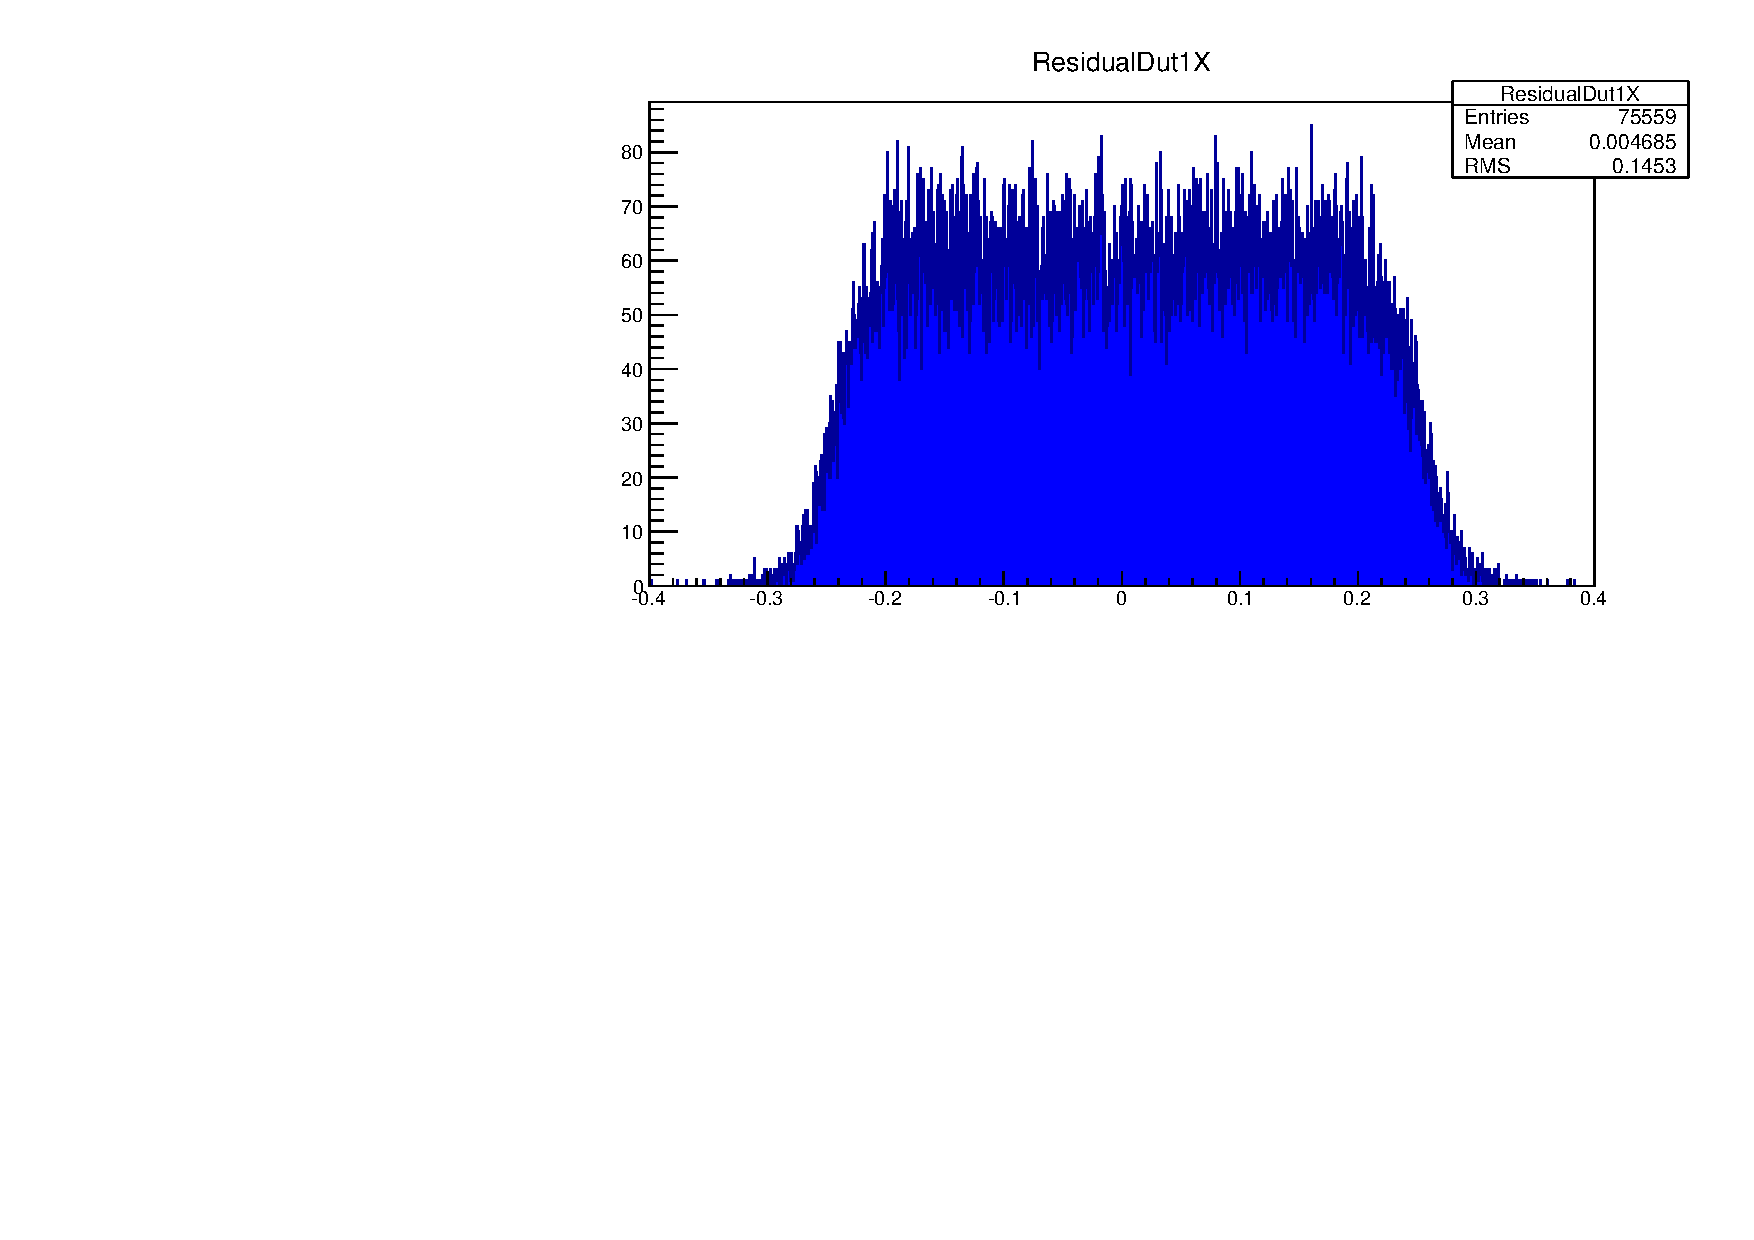
\includegraphics[scale=0.5]{figures/resX1D21.pdf}}
\subfloat{\label{fig:beamE5B1} 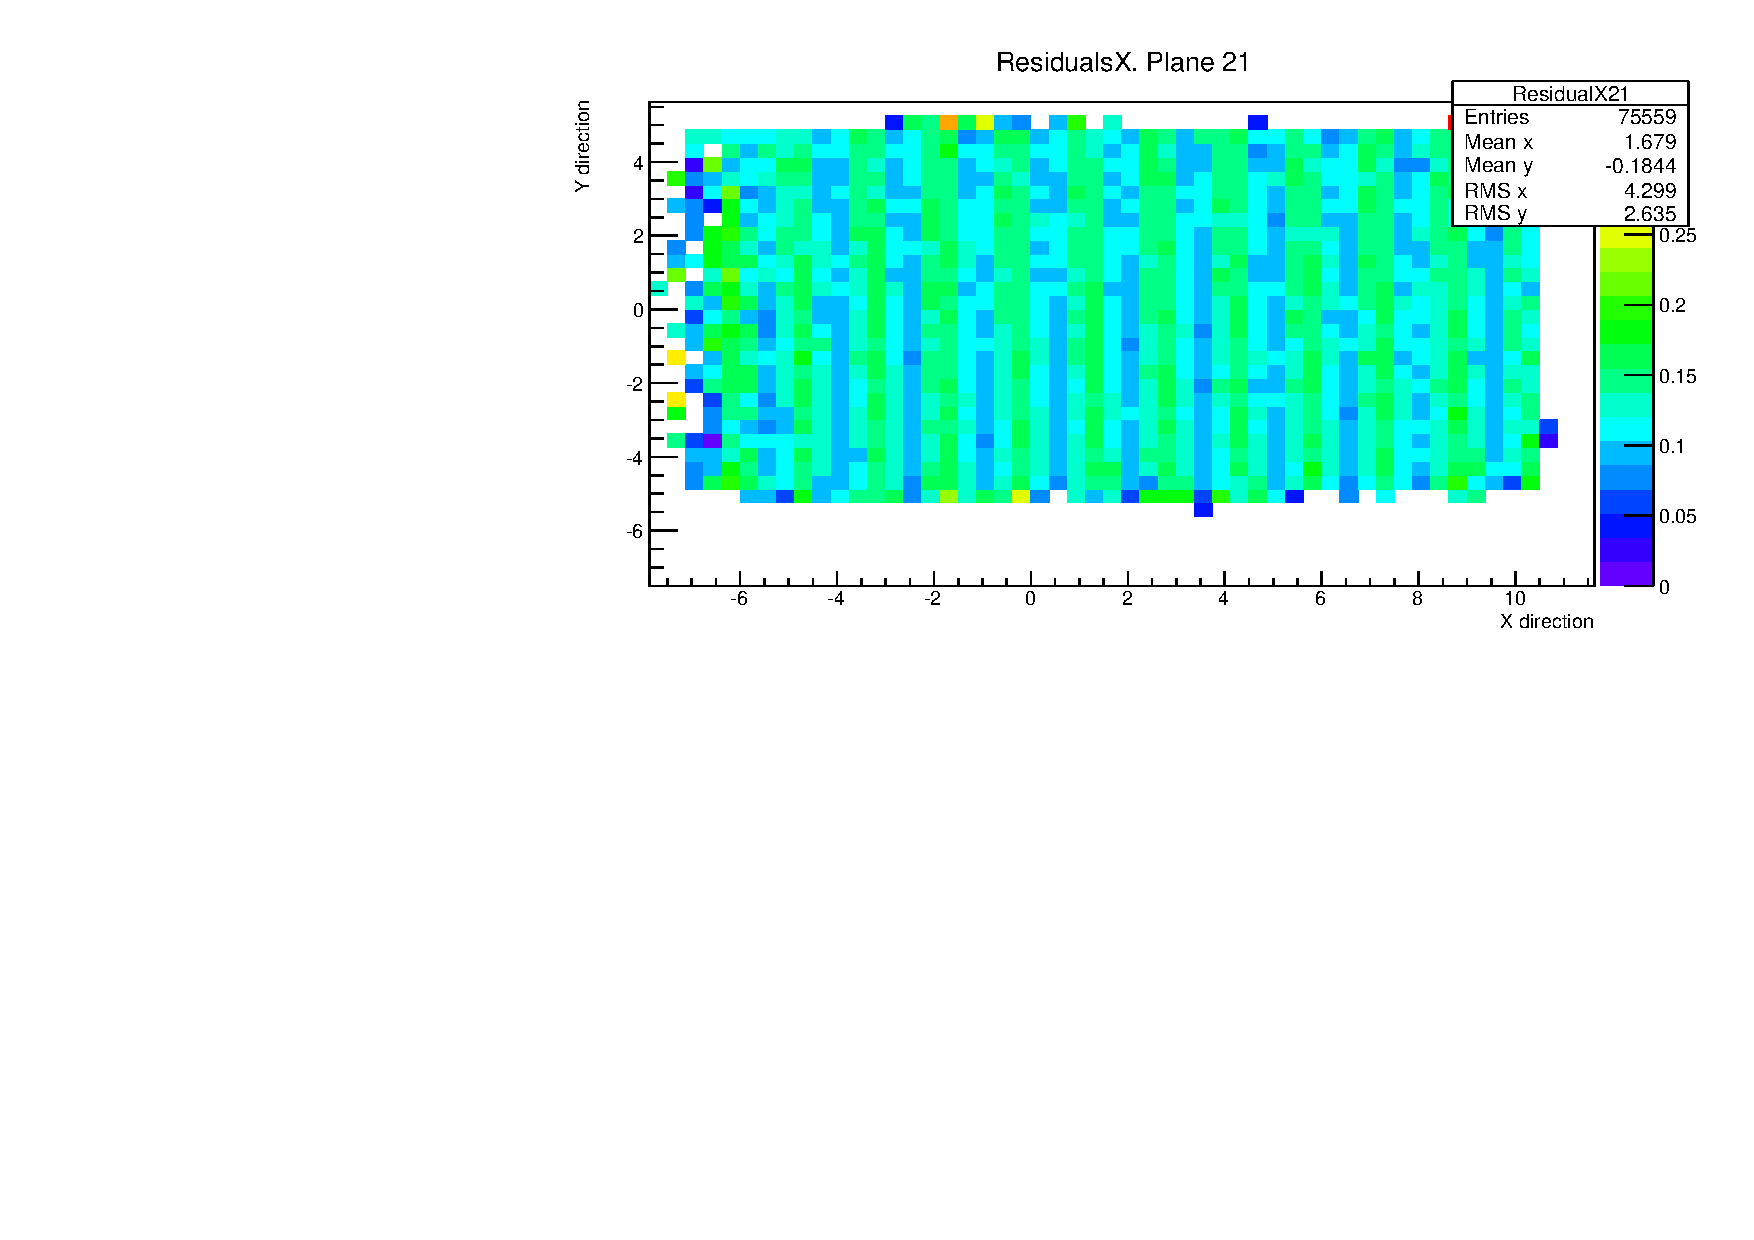
\includegraphics[scale=0.5]{figures/XRes2D21.pdf}}
\caption{The residual from plane 21 inclusive and over the detector surface. DESY testbeam 4 GeV}
\label{fig:kinkRad}
\end{figure}


\subsection{SCT strip}

\subsection{Alibava strip}

\subsection{Magnetic fields (no DUT)}

\subsection{X0}

\newpage

\begin{figure}[H]
\hspace{-35mm}
\subfloat{\label{fig:beamE5B1} 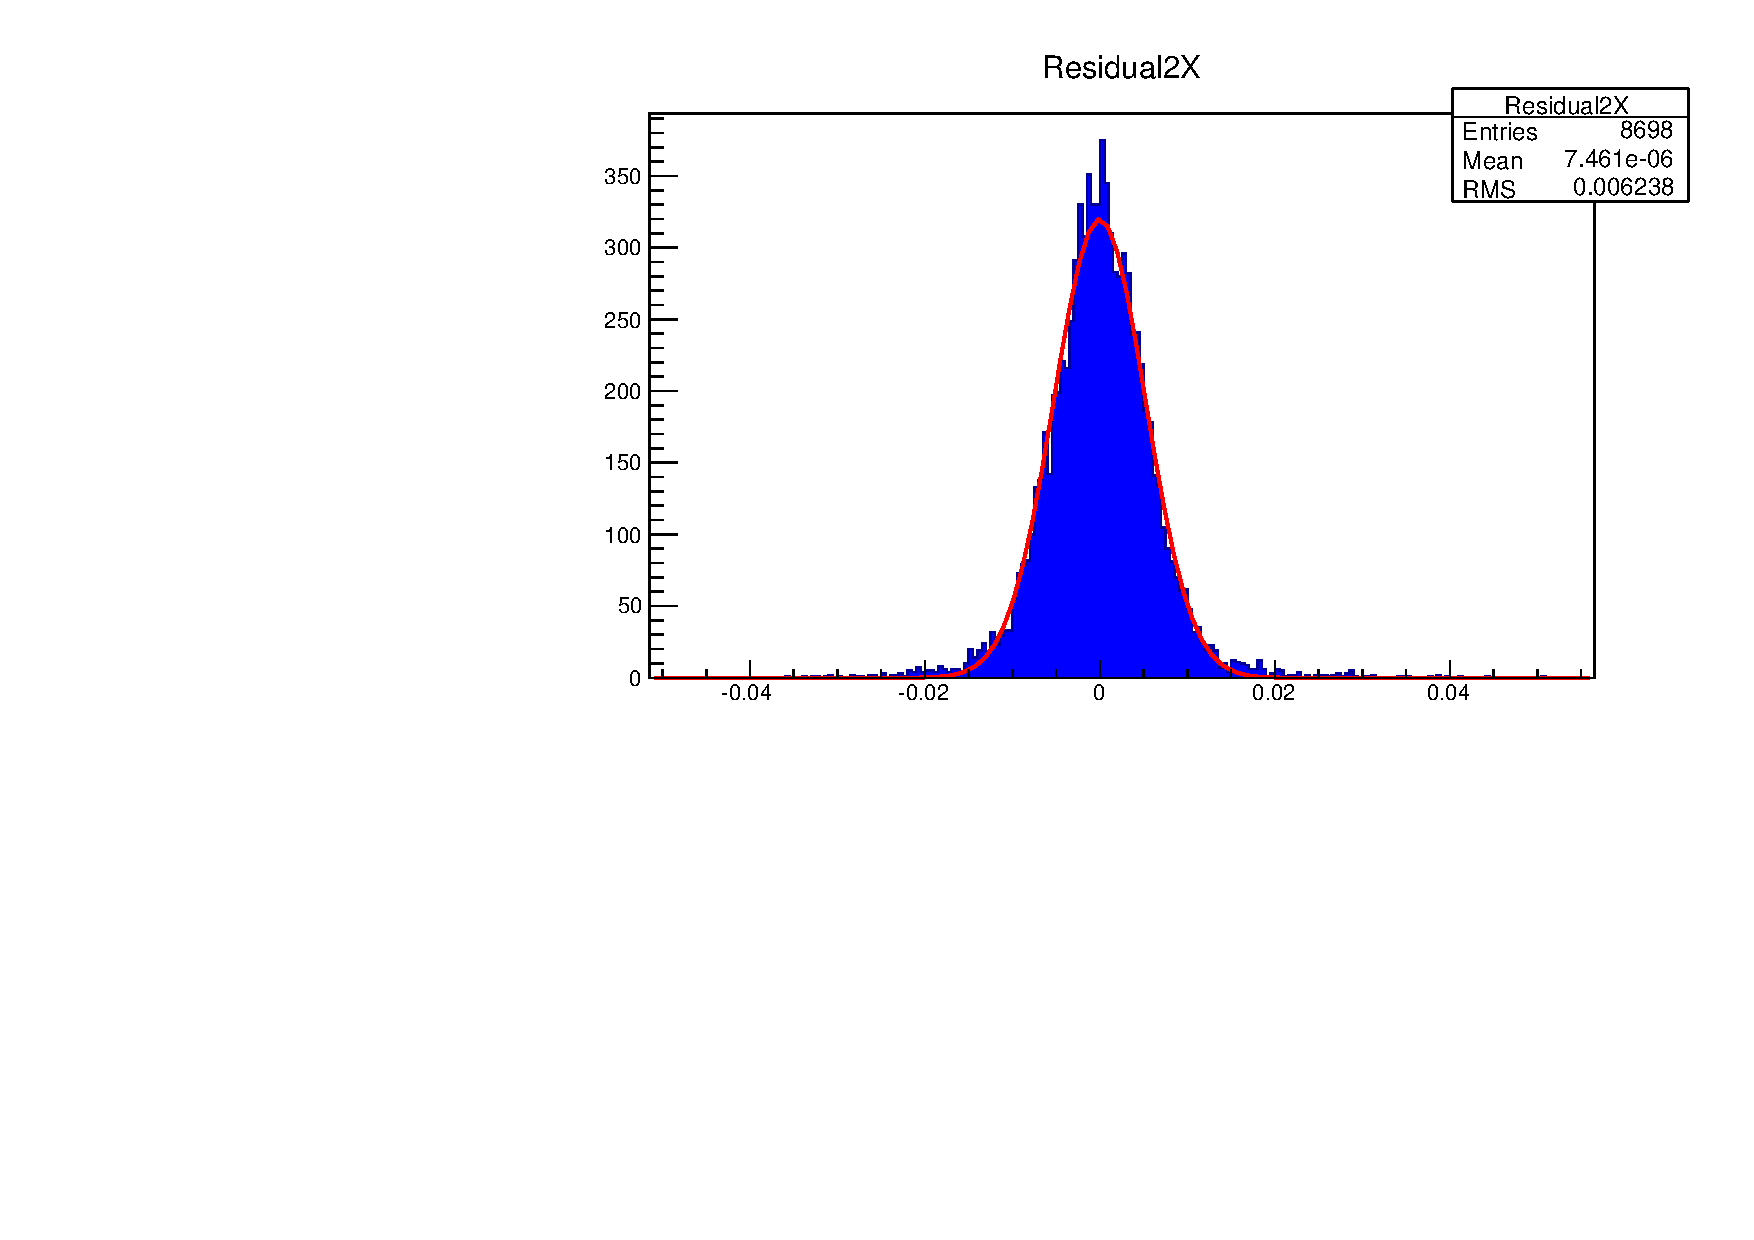
\includegraphics[scale=0.5]{figures/Sensor241-plane2ExcludeXRes.pdf}}
\subfloat{\label{fig:beamE5B1} 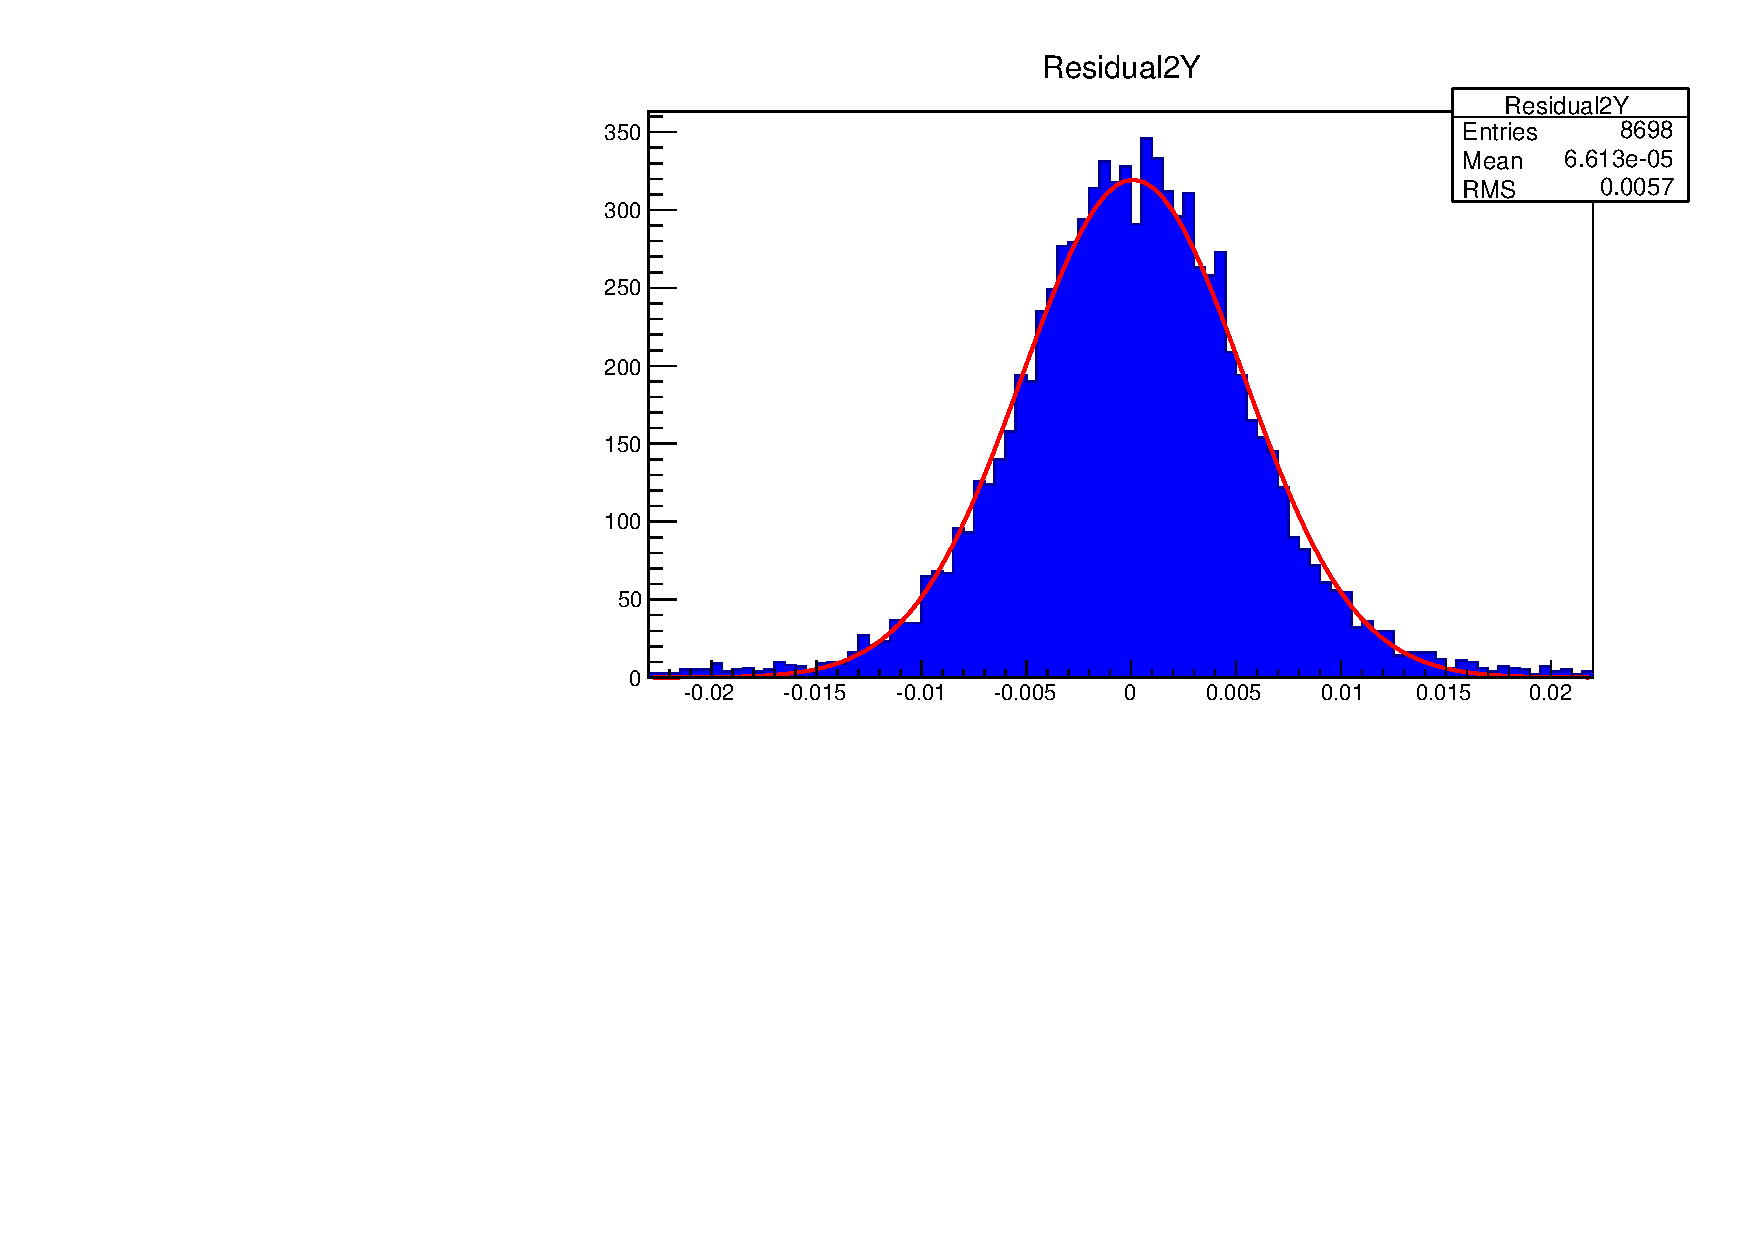
\includegraphics[scale=0.5]{figures/241-plane2ExcludeYRes.pdf}}
\caption{}
\label{fig:energy0}
\end{figure}

\begin{figure}[H]
\hspace{-35mm}
\subfloat{\label{fig:beamE5B1} 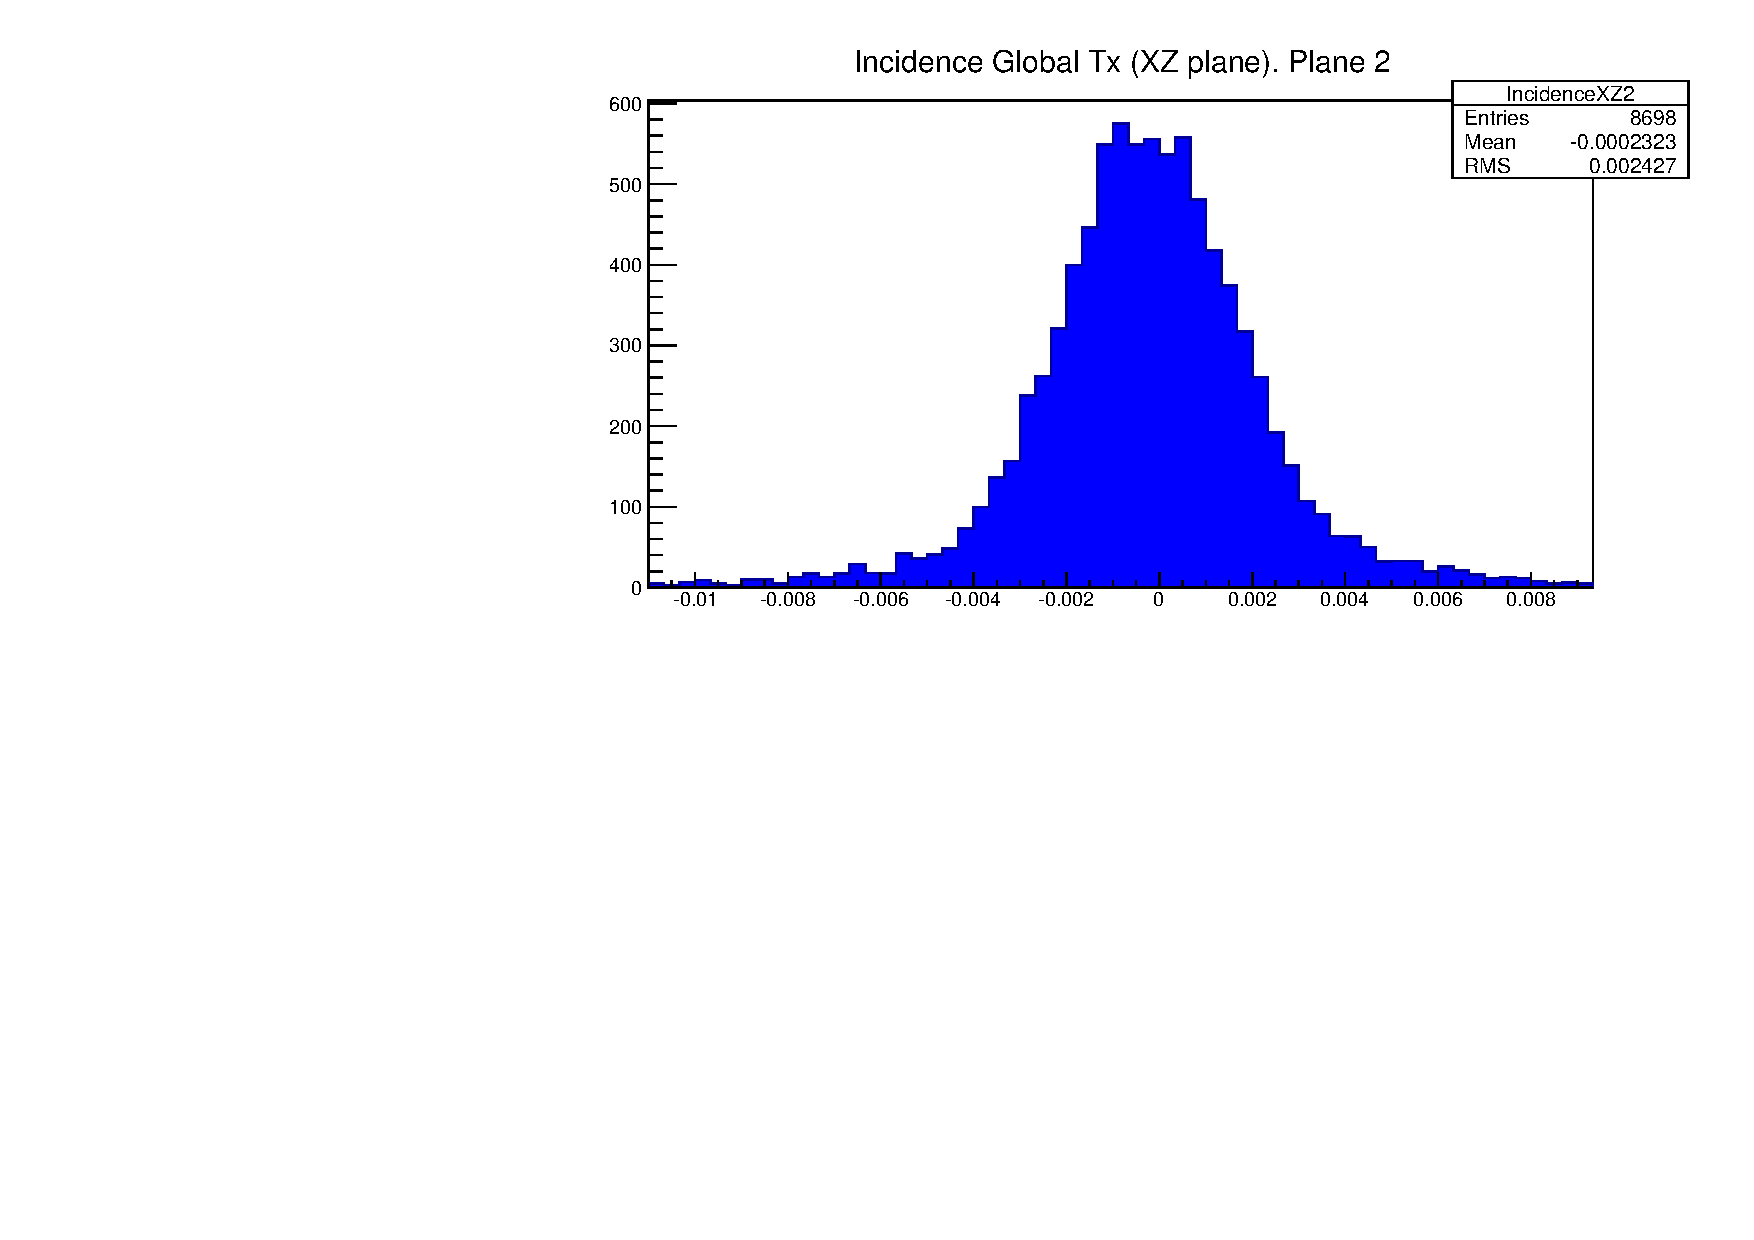
\includegraphics[scale=0.5]{figures/241-plane2ExcludeXInc.pdf}}
\subfloat{\label{fig:beamE5B1} 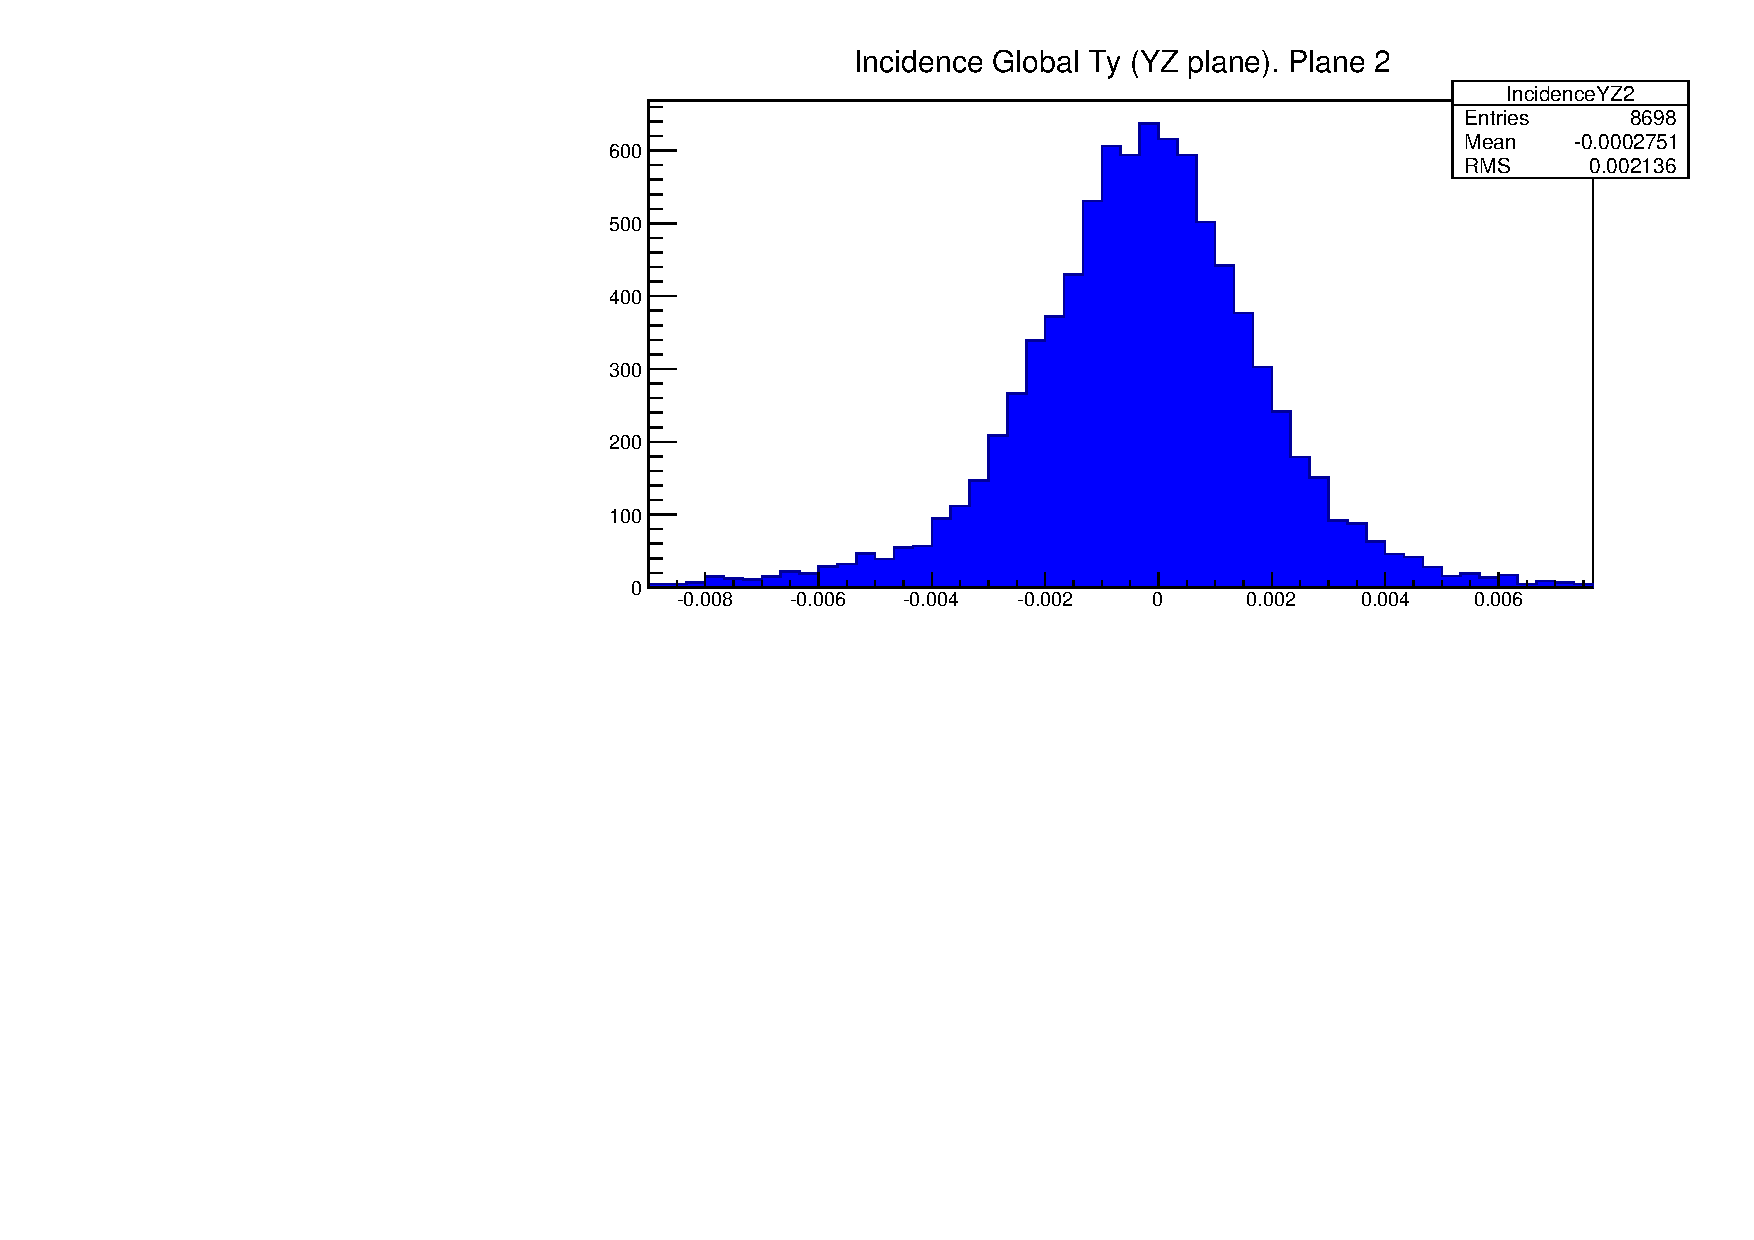
\includegraphics[scale=0.5]{figures/241-plane2ExcludeYInc.pdf}}
\caption{}
\label{fig:energy0}
\end{figure}


\begin{figure}[H]
\hspace{-35mm}
\subfloat{\label{fig:beamE5B1} 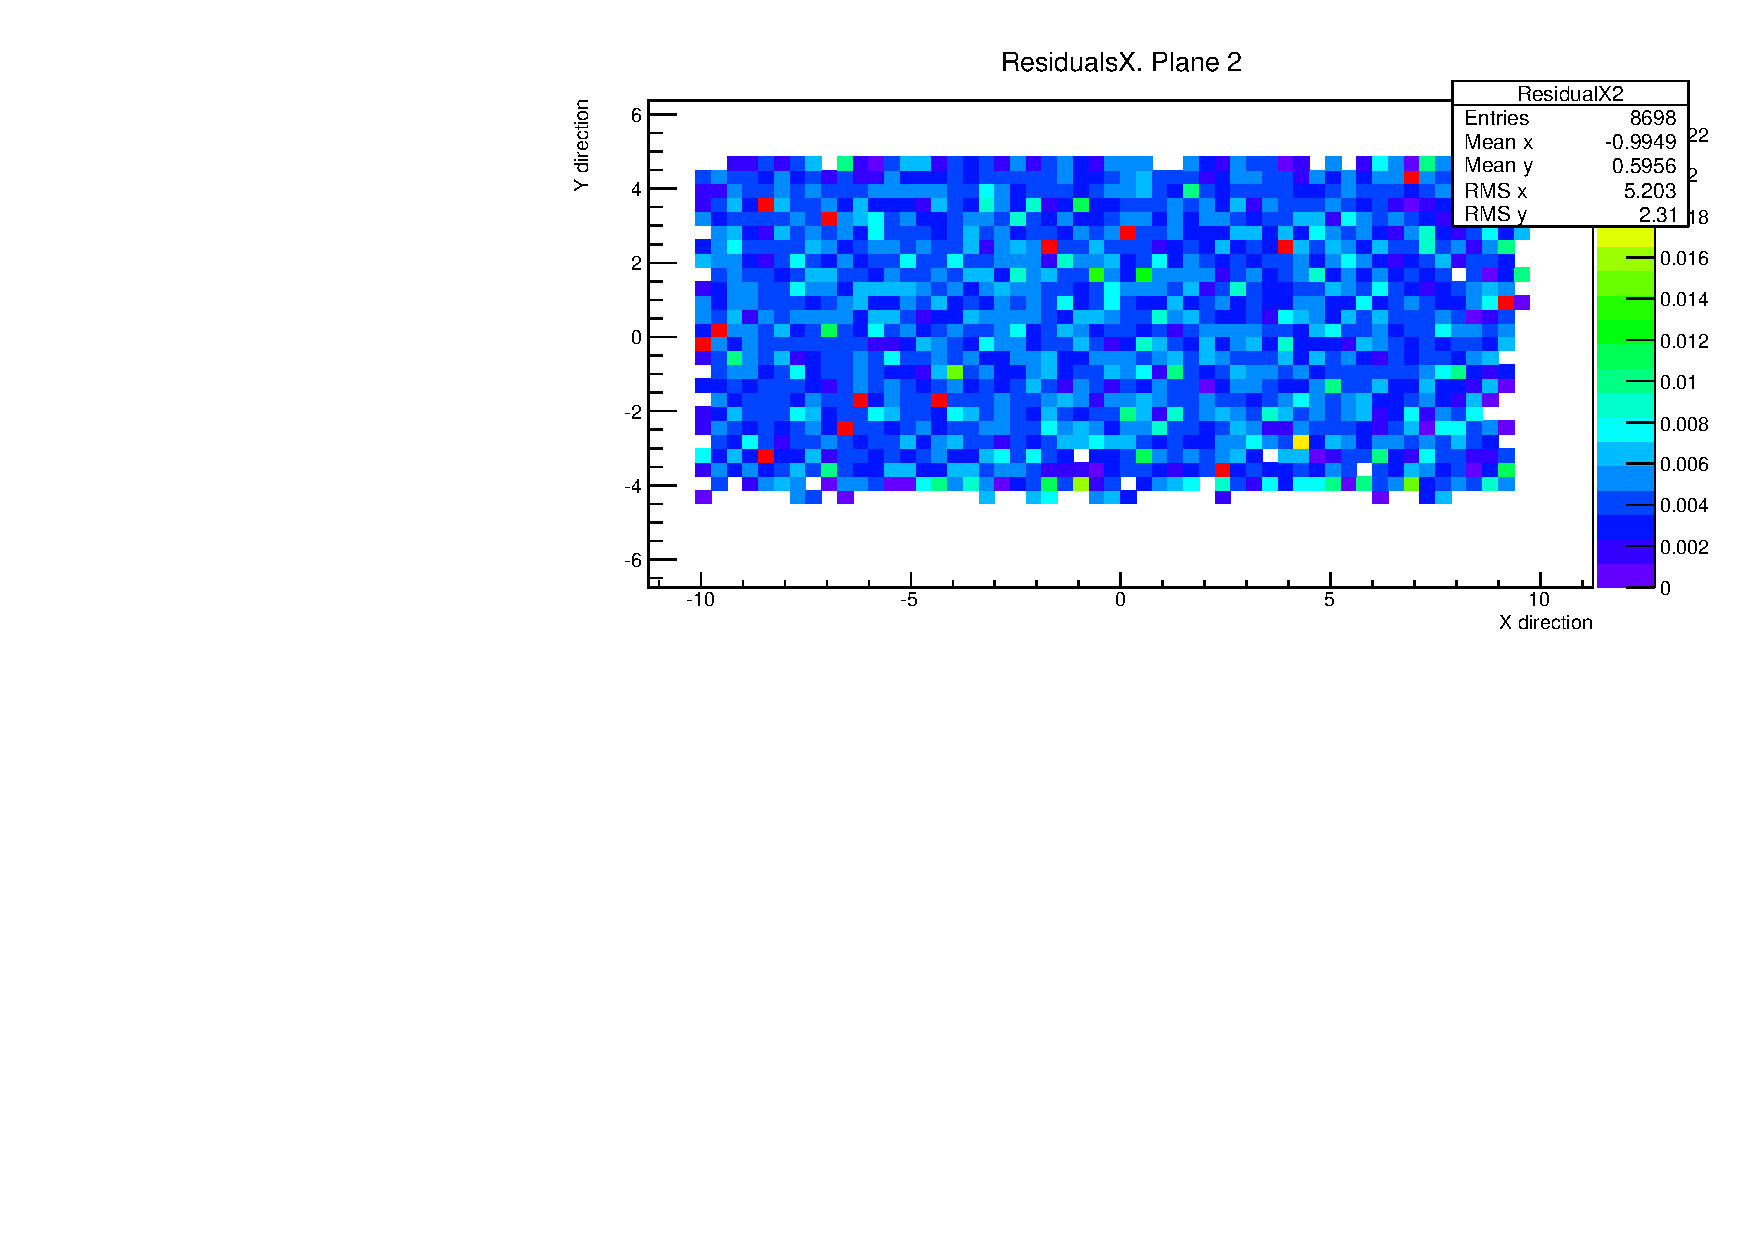
\includegraphics[scale=0.5]{figures/241-plane2ExcludeXRes2D.pdf}}
\subfloat{\label{fig:beamE5B1} 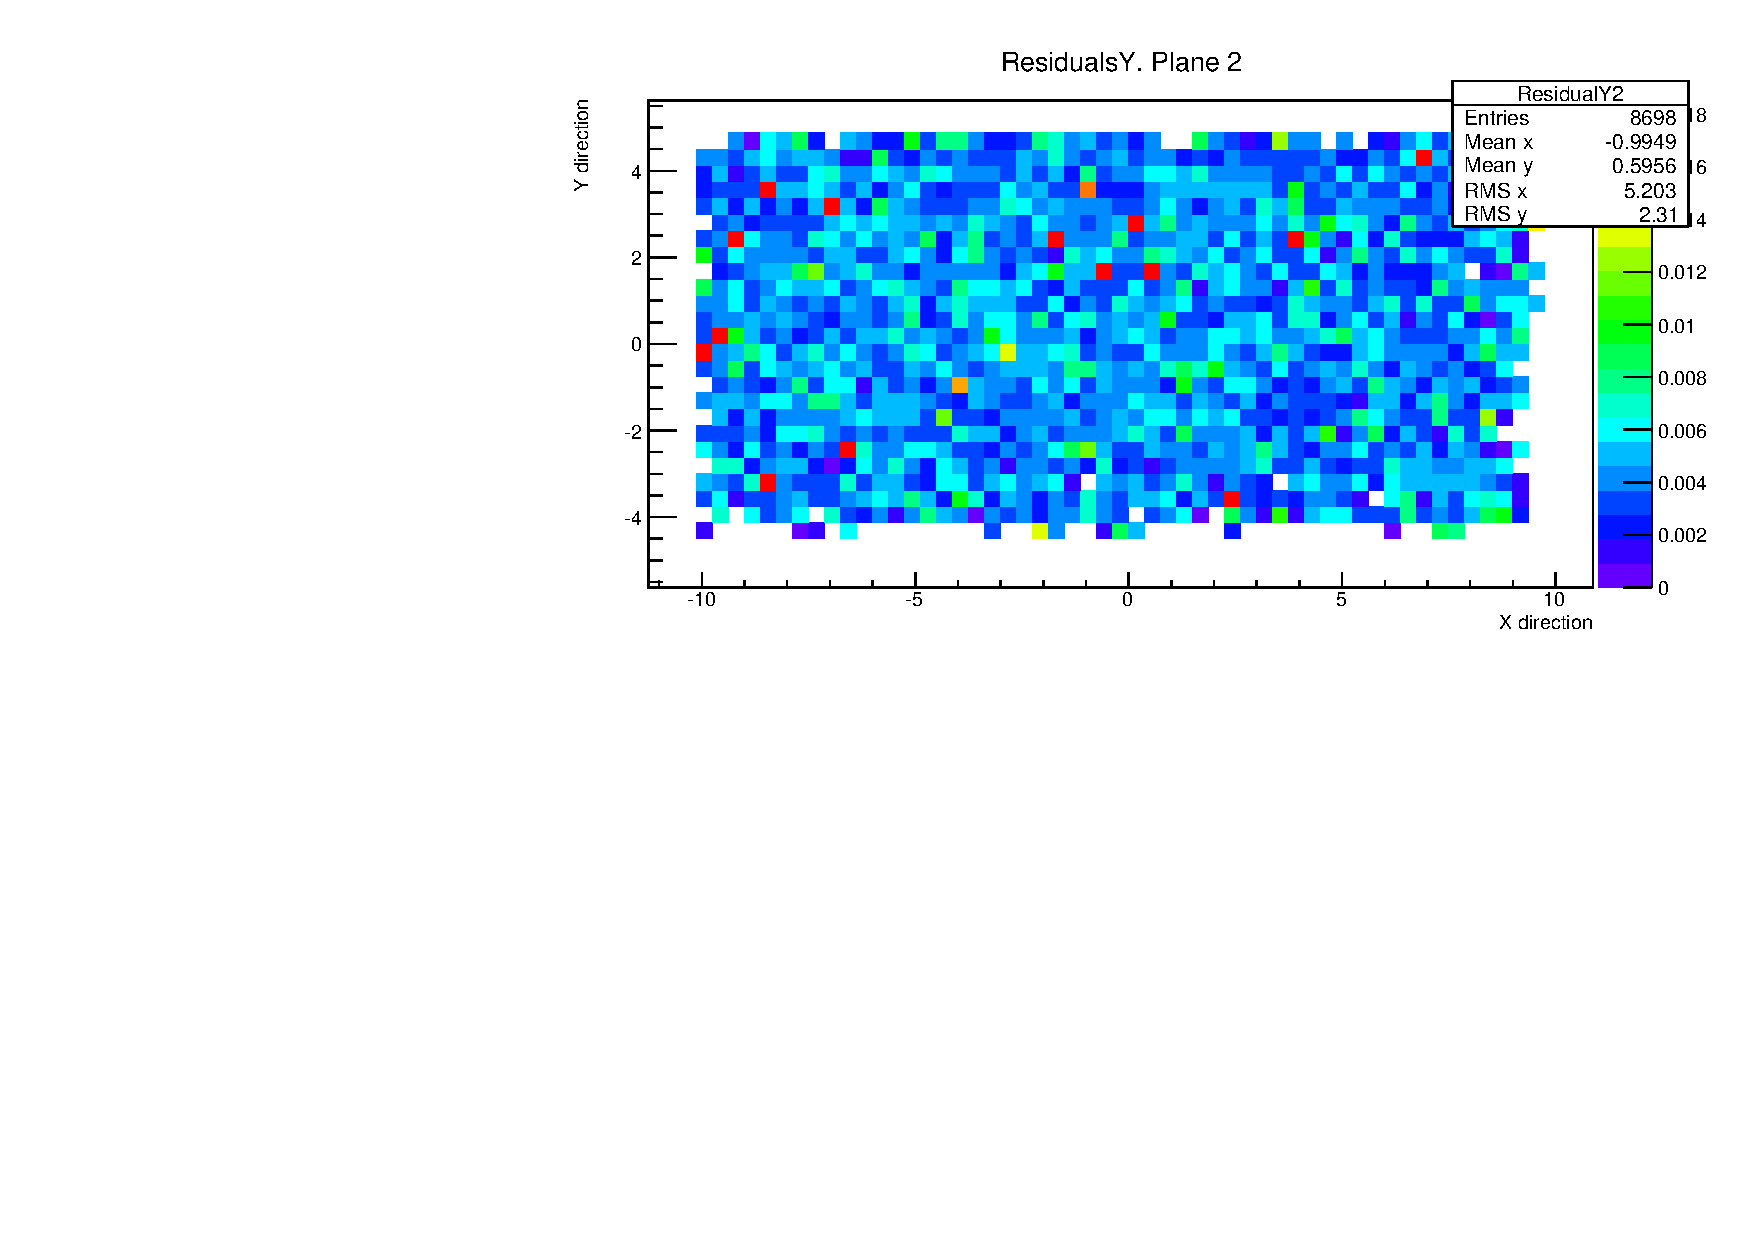
\includegraphics[scale=0.5]{figures/241-plane2ExcludeYRes2D.pdf}}
\caption{}
\label{fig:energy0}
\end{figure}

\begin{figure}[H]
\hspace{-35mm}
\subfloat{\label{fig:beamE5B1} 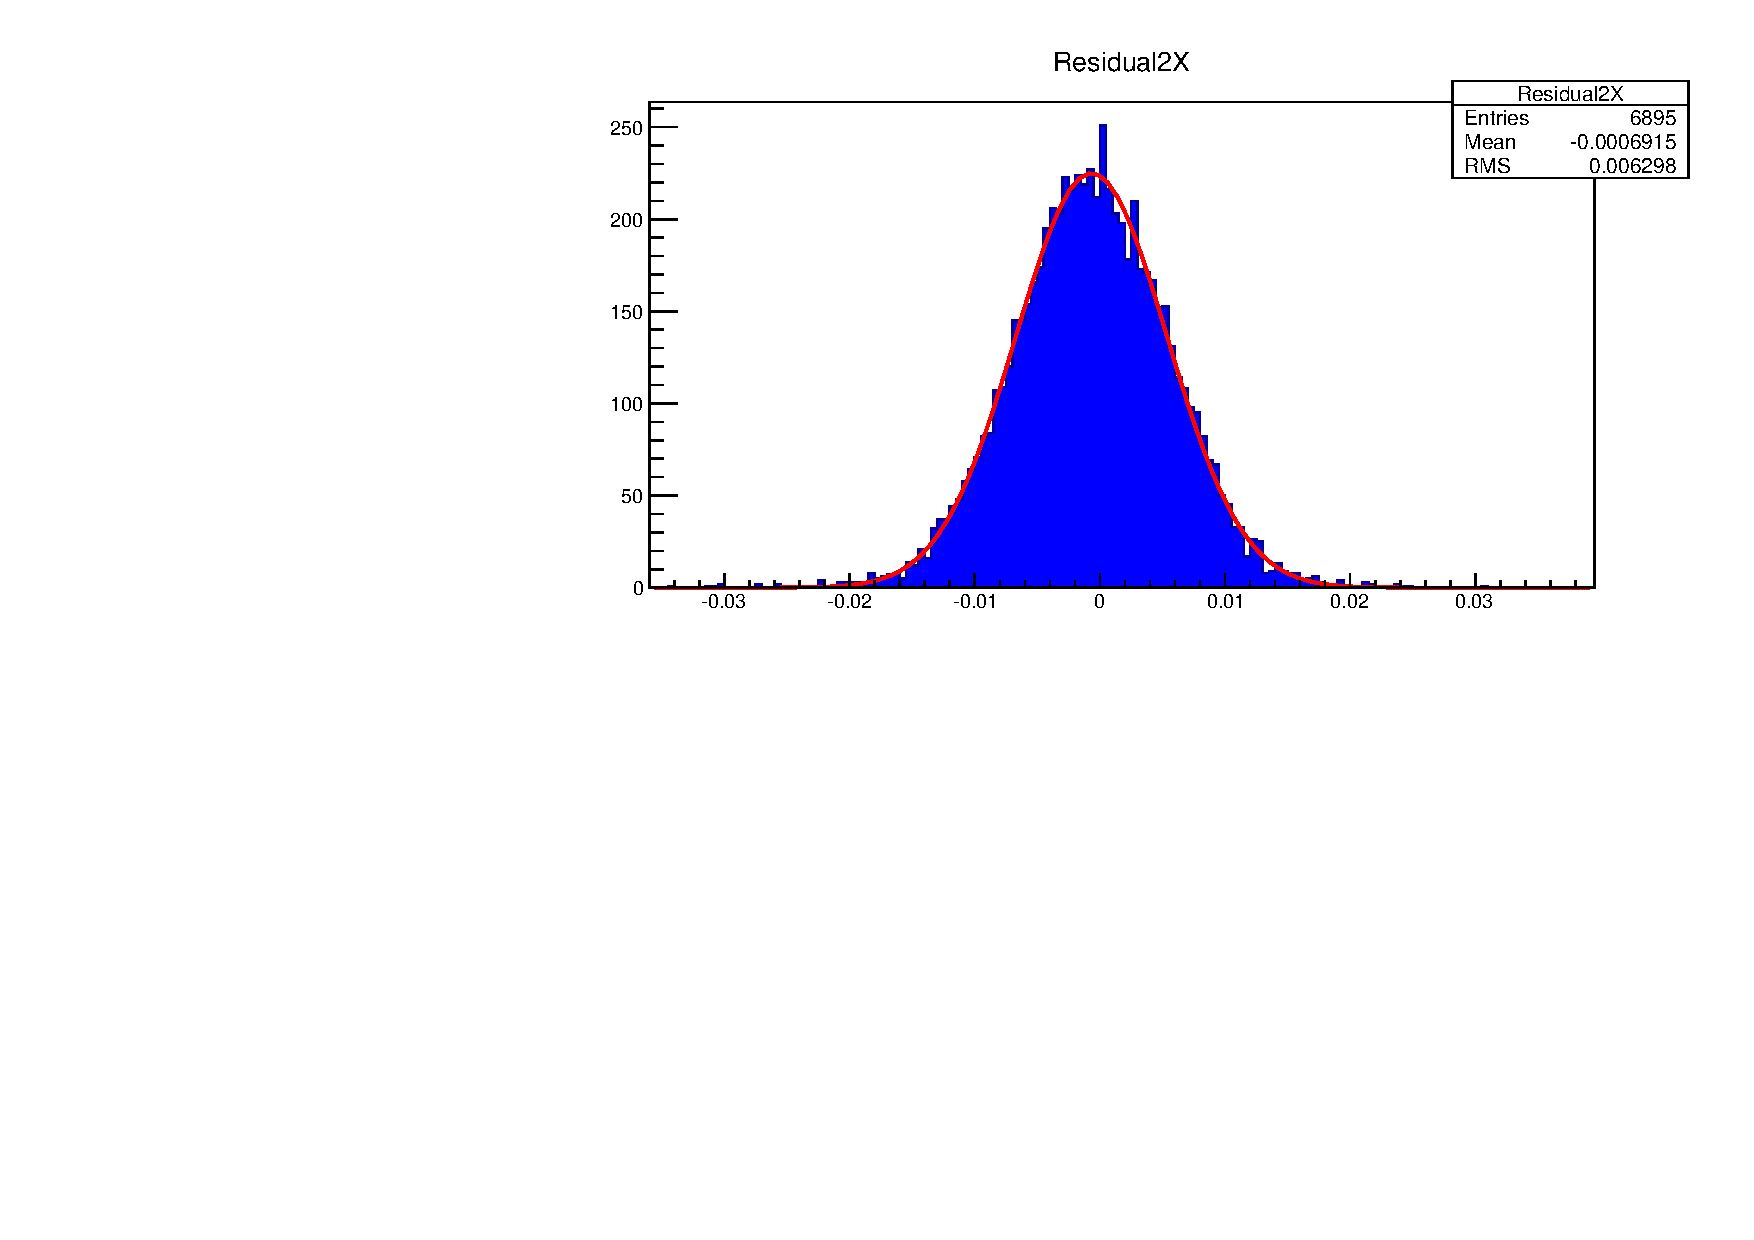
\includegraphics[scale=0.5]{figures/resX286-plane2Exc.pdf}}
\subfloat{\label{fig:beamE5B1} 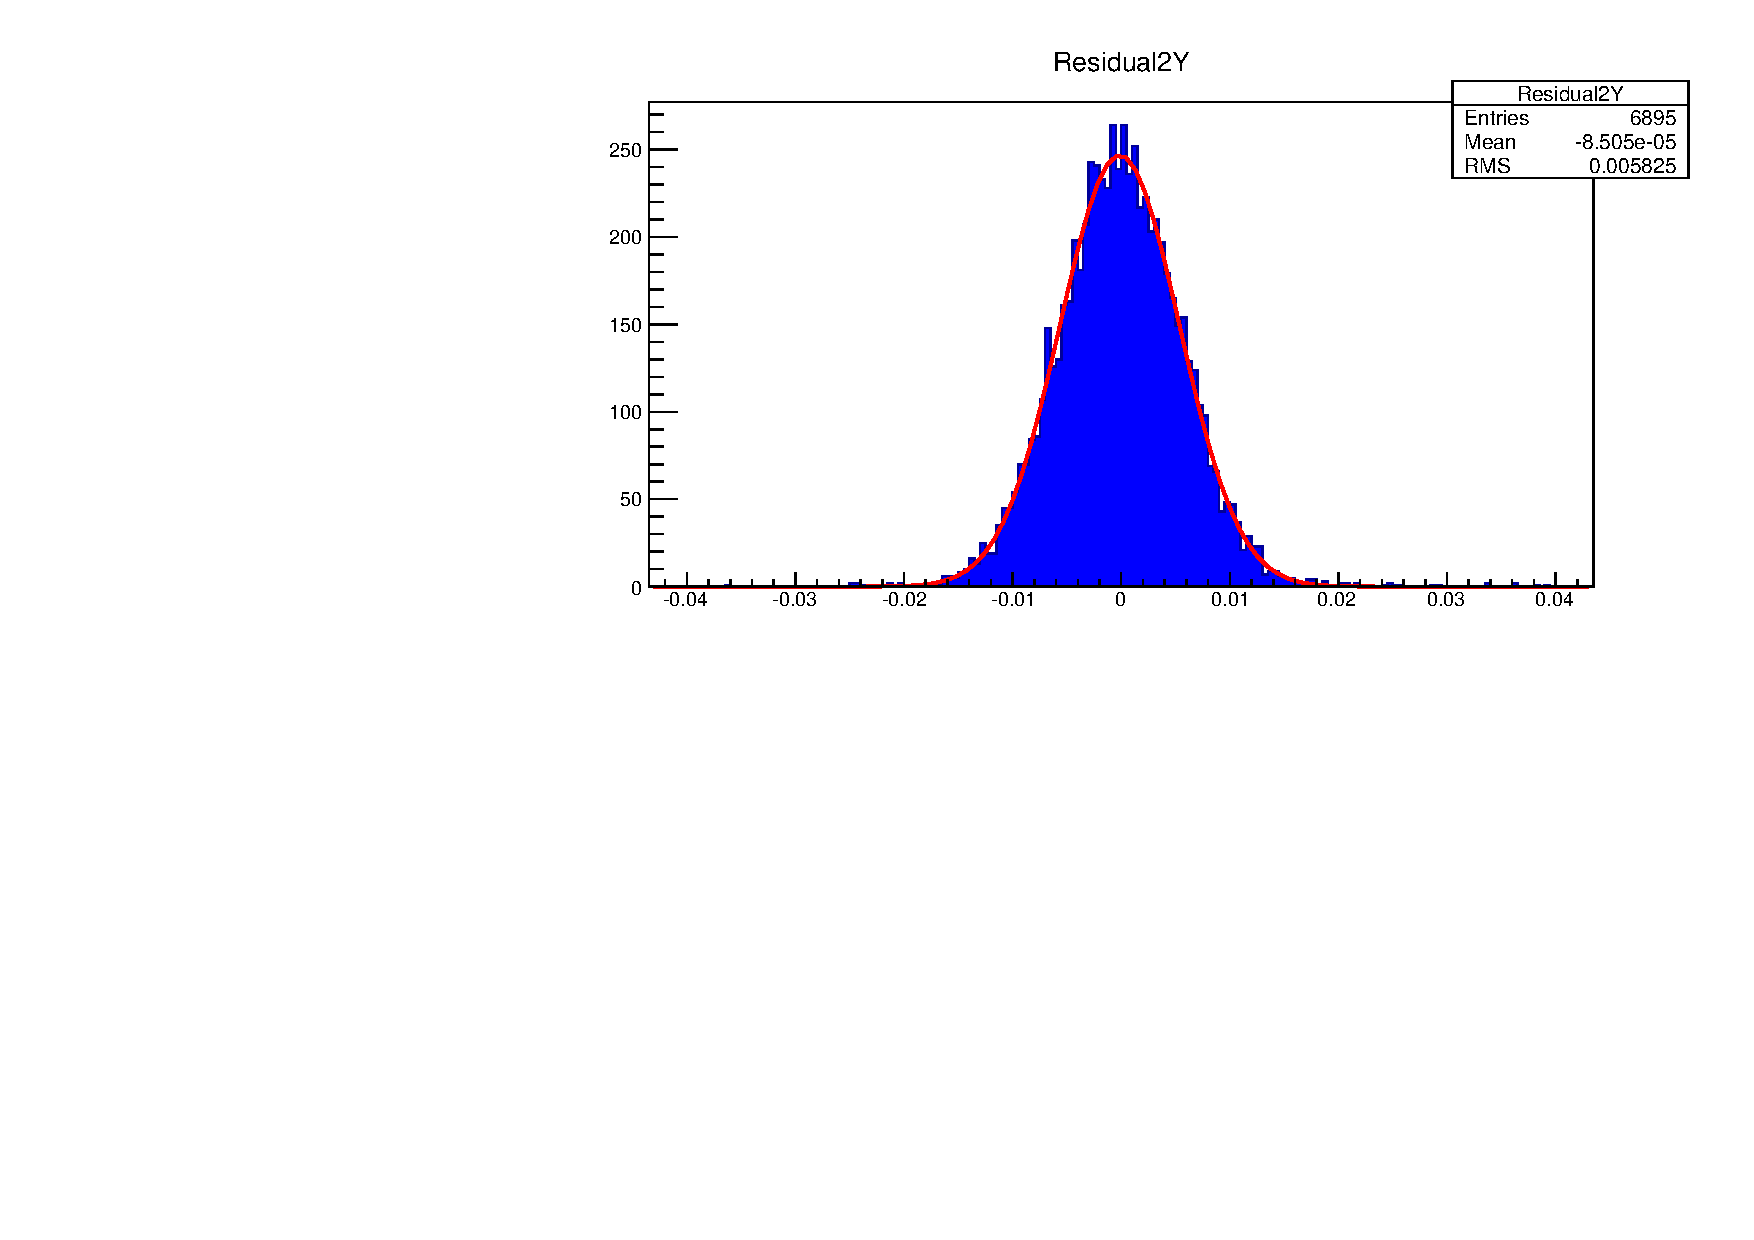
\includegraphics[scale=0.5]{figures/resY286-plane2Exc.pdf}}
\caption{}
\label{fig:energy0}
\end{figure}

\begin{figure}[H]
\hspace{-35mm}
\subfloat{\label{fig:beamE5B1} 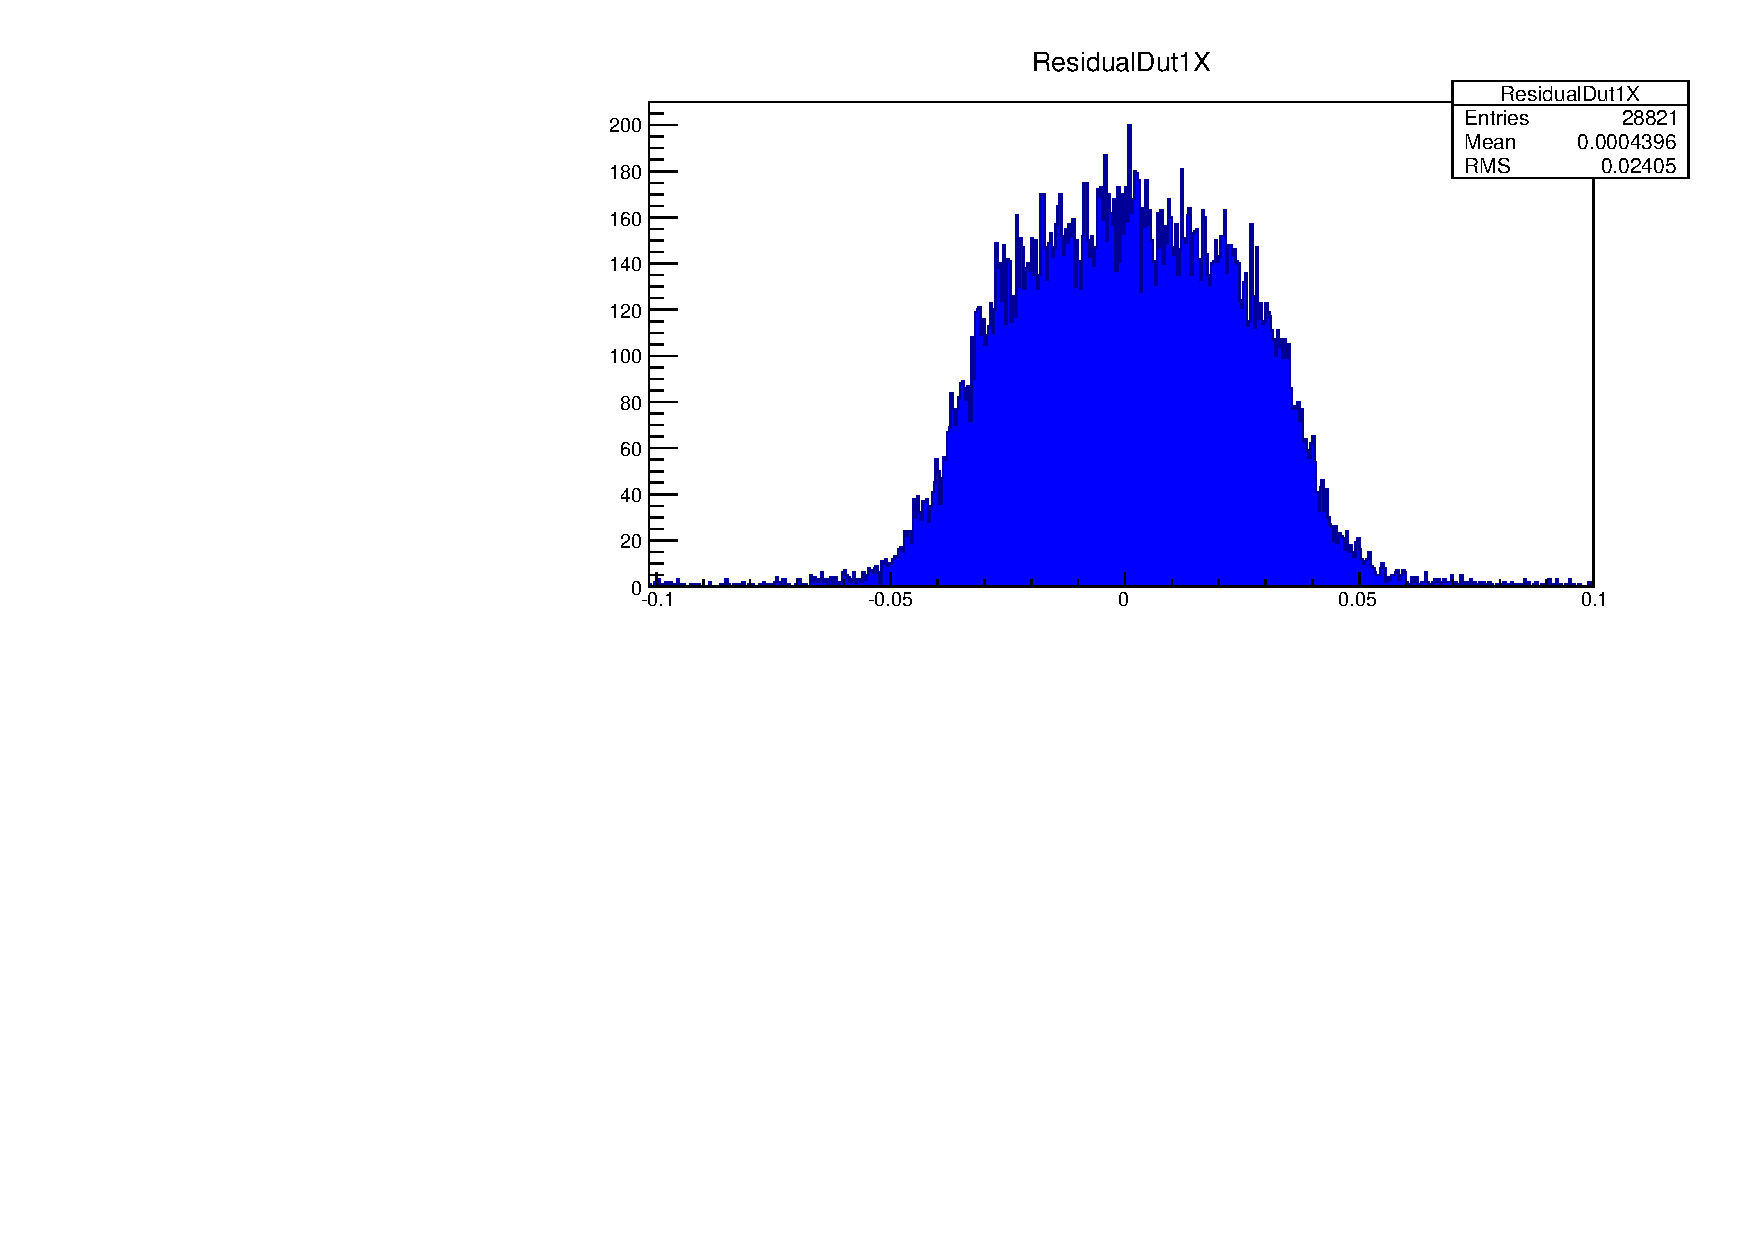
\includegraphics[scale=0.5]{figures/strip703Res.pdf}}
\subfloat{\label{fig:beamE5B1} 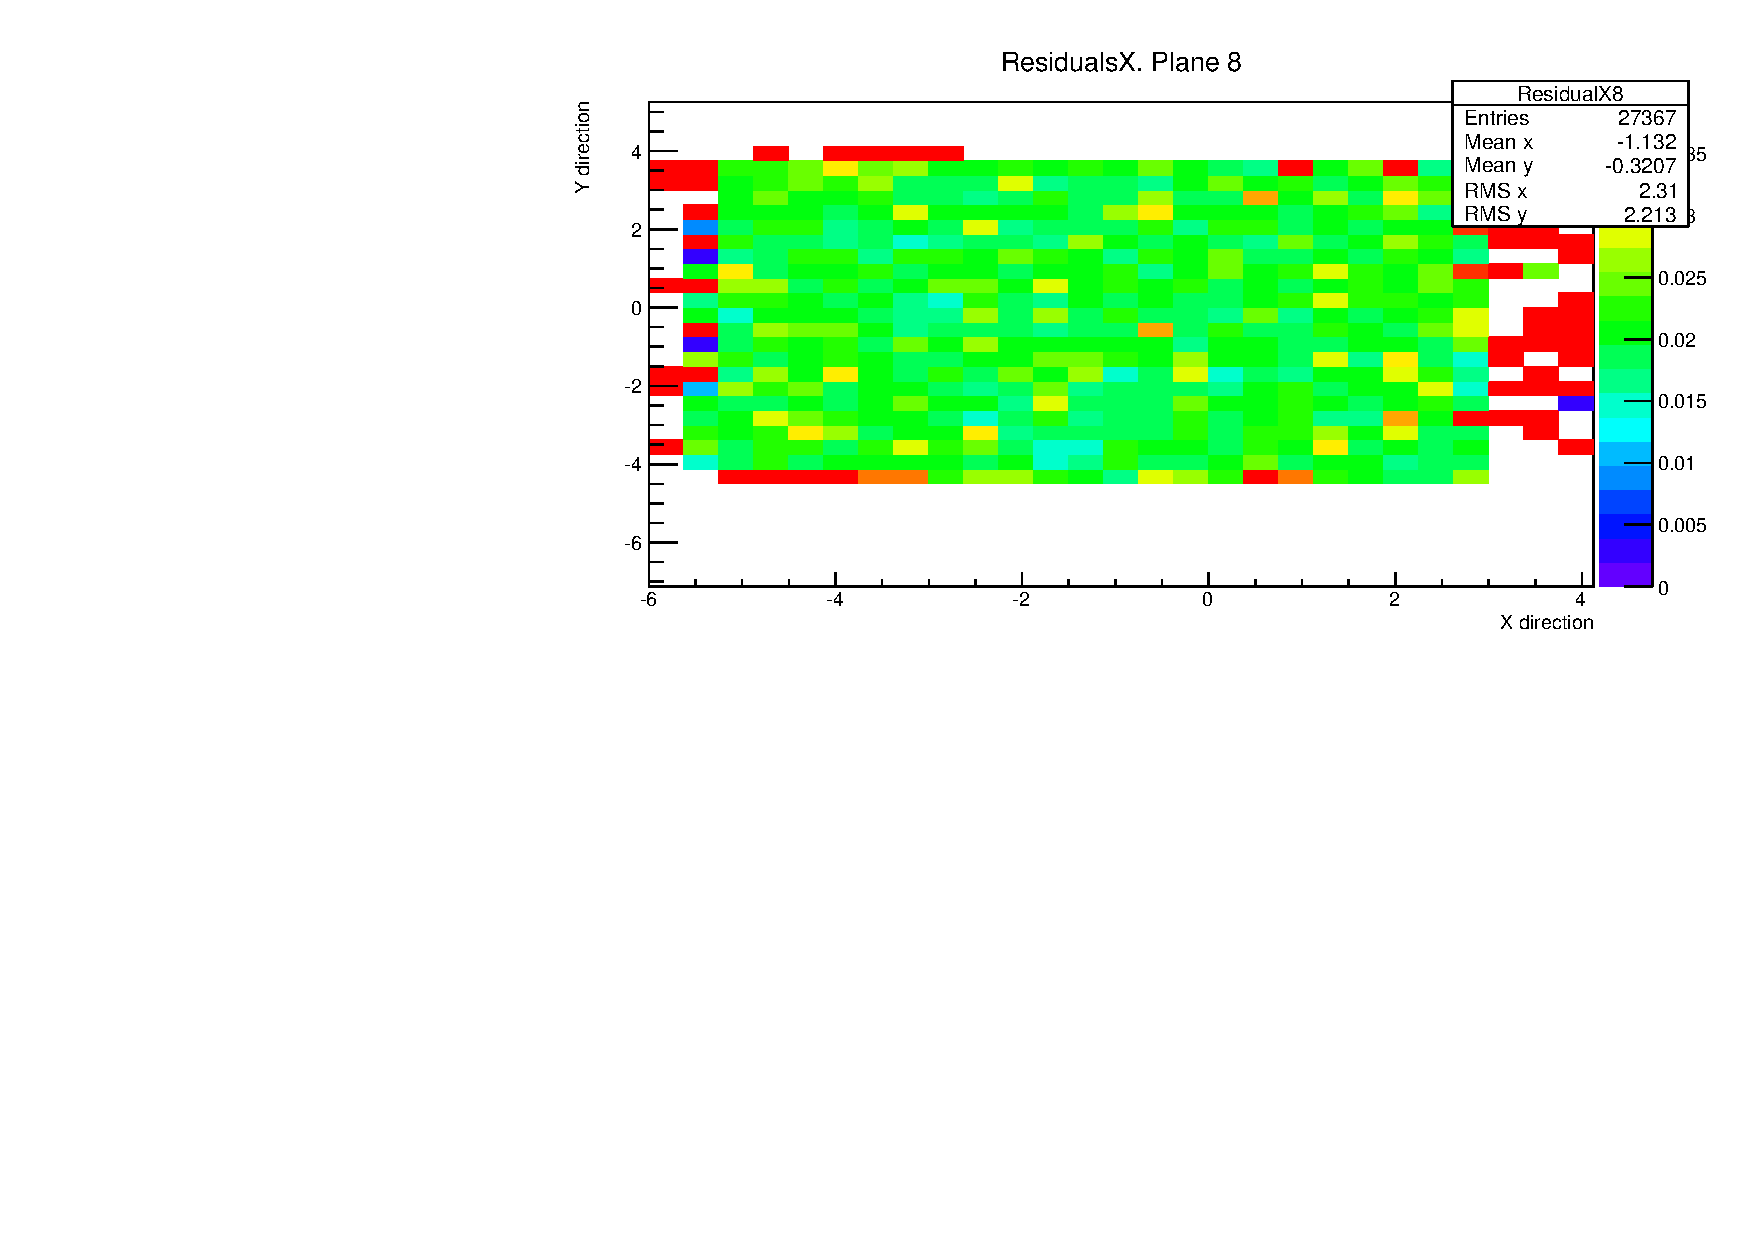
\includegraphics[scale=0.5]{figures/strip703Res2D.pdf}}
\caption{}
\label{fig:energy0}
\end{figure}




\subsection{Examples.}

%This can be seen as the relationship between moving a track a particular displacement and its intersection with a plane.


%The \emph{point correction matrix} $PC(X,Y,Z, \alpha,\beta,\gamma)$ is of the from.
%\[ \left( \begin{array}{cccccc}%
%1 & 0 & \frac{\partial d_0}{\partial d_2}   \\
%0 & 1 & \frac{\partial d_1}{\partial d_2}  \\
%\end{array} \right)\] 







